% SI Section One: Additional details on DFT calculations
% Tables are formatted following: https://tex.stackexchange.com/questions/254254/how-to-set-figures-and-tables-captions-in-apa-style-without-using-apa6-class

\section{Additional details on DFT calculations}

\subsection{Catalyst models}
\label{supp_sec2.1_catalysts}

Representative structures for each substrate are depicted in \cref{supp_fig2:Ge_g-C3N4} through \cref{supp_fig7:Al-C2N}. For the adsorption process, the initial state is defined by positioning the optimized adsorbates at a distance of 6.5 \text{\AA} from the single-metal atoms supported on the substrate, oriented along the z-axis.

% SI Figure 1: Periodic table of investigated metals
\begin{figure}[htbp]
  \centering
  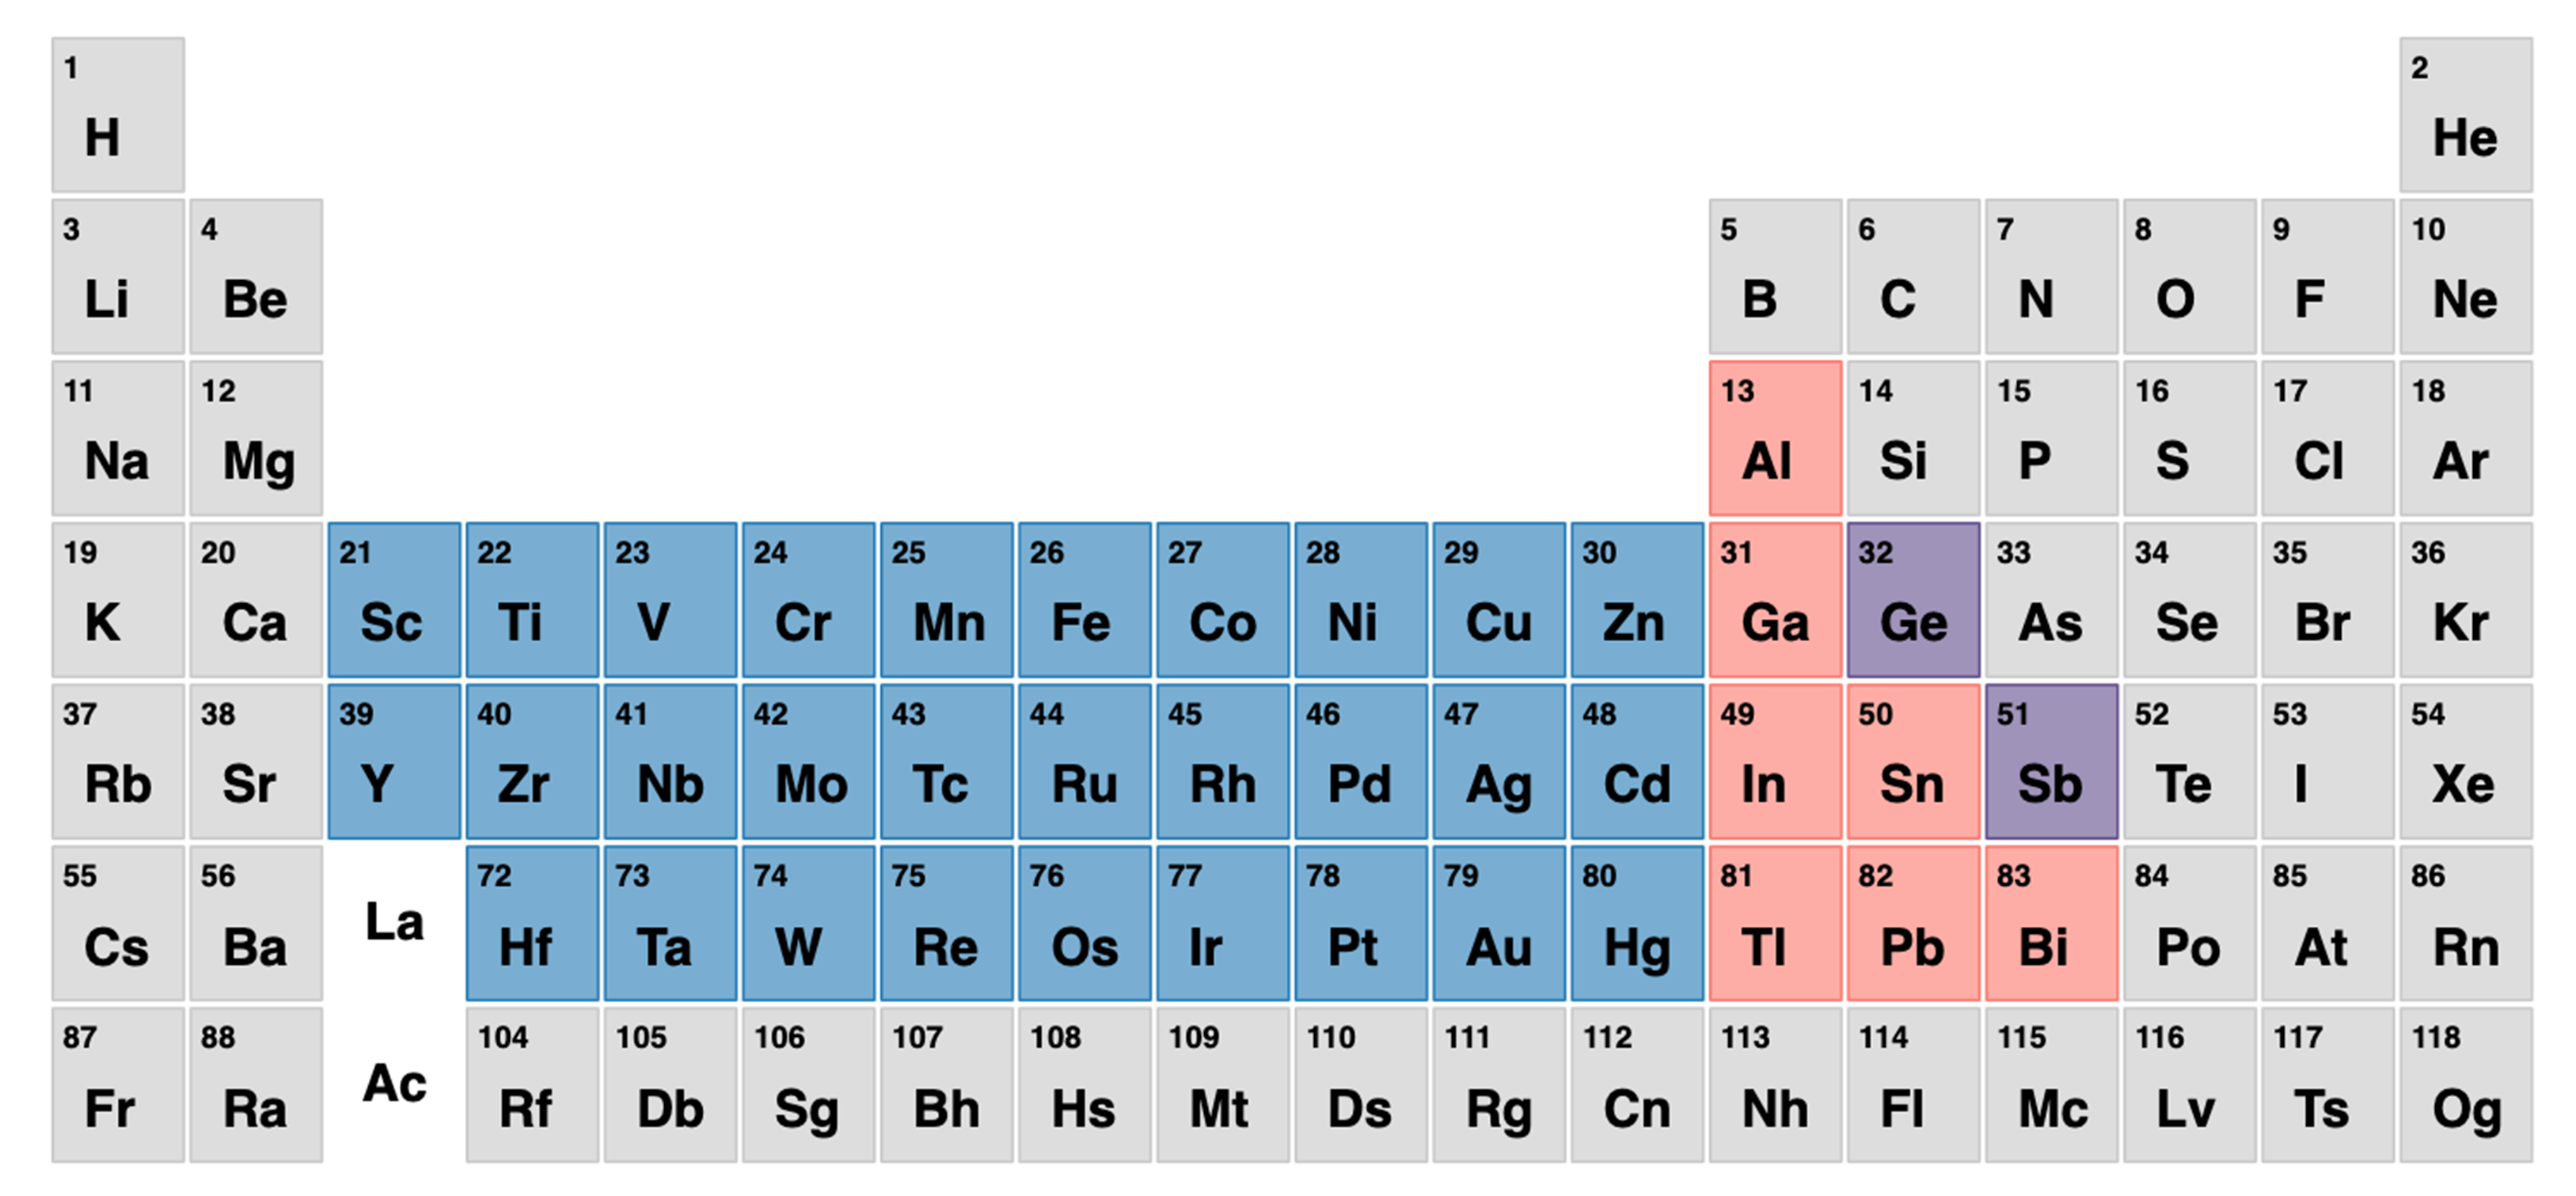
\includegraphics[width=\textwidth]{supp_fig1_ptable.png}
  \caption{\textbf{Periodic table of investigated metals.}
  Periodic table highlighting investigated elements: transition metals in blue, metalloids in purple, and other metals in orange.}
  \label{supp_fig1:ptable}
\end{figure}

% SI Figure 2: Structure of Ge atom supported on g-C3N4
\begin{figure}[htbp]
  \centering
  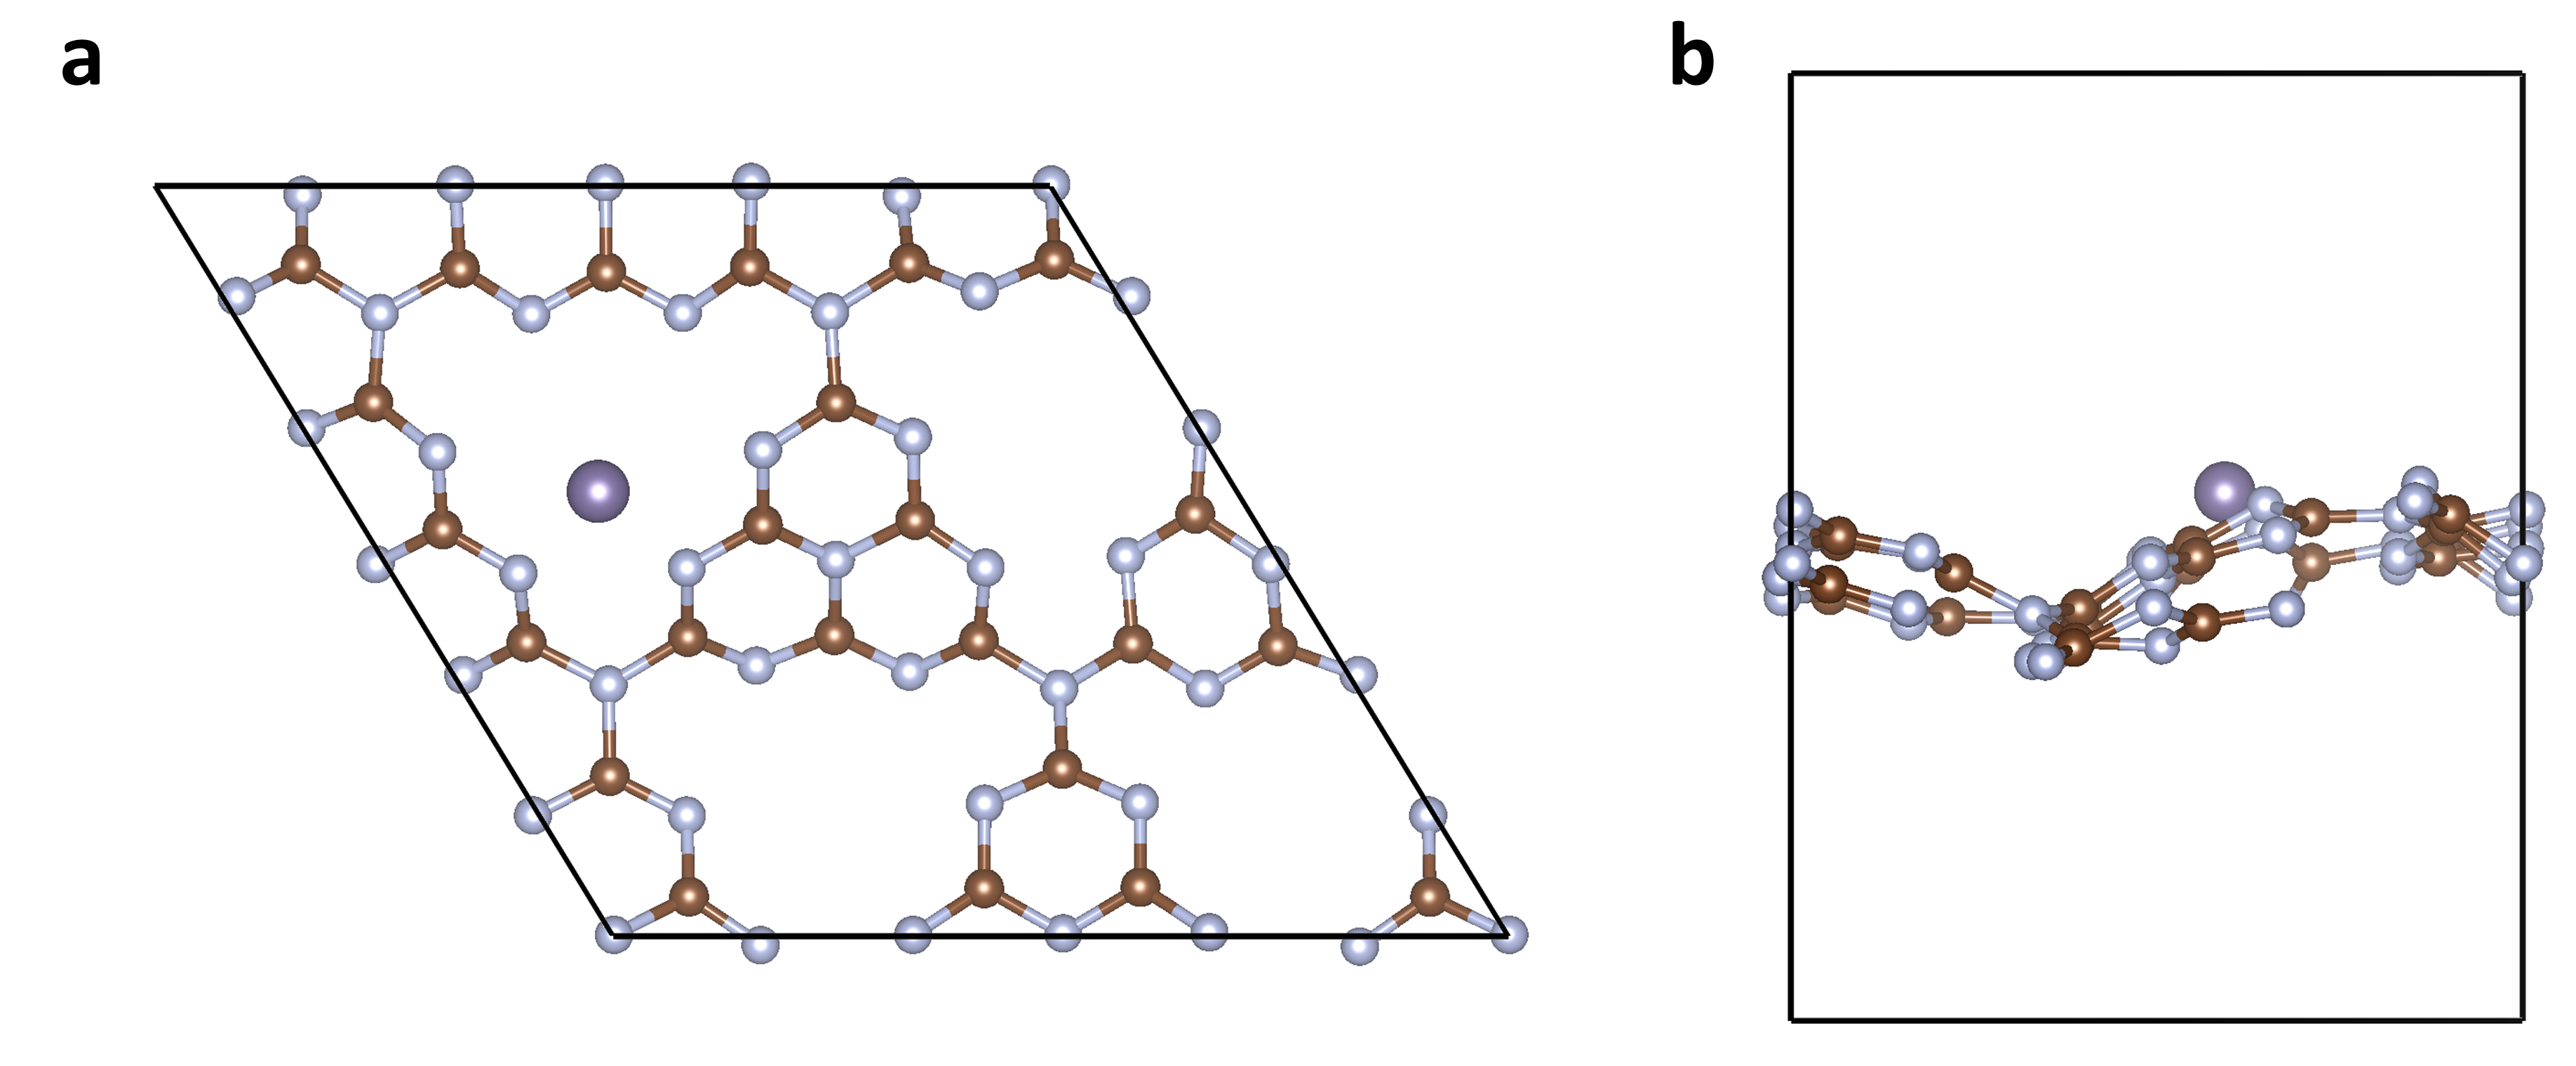
\includegraphics[width=\textwidth]{supp_fig2_Ge_g-C3N4.png}
  \caption{\textbf{Structure of single germanium atom supported on graphitic nitride.}
  (\textbf{a}) View along the z-axis and (\textbf{b}) view along the x-axis
  of the Ge@g-C\textsubscript{3}N\textsubscript{4} structure.
  In the illustrations, silver spheres represent N atoms, brown spheres
  signify C atoms, and purple sphere indicates Ge atom.}
  \label{supp_fig2:Ge_g-C3N4}
\end{figure}

% SI Figure 3: Structure of Cr atom supported on nitrogen-doped graphene
\begin{figure}[htbp]
  \centering
  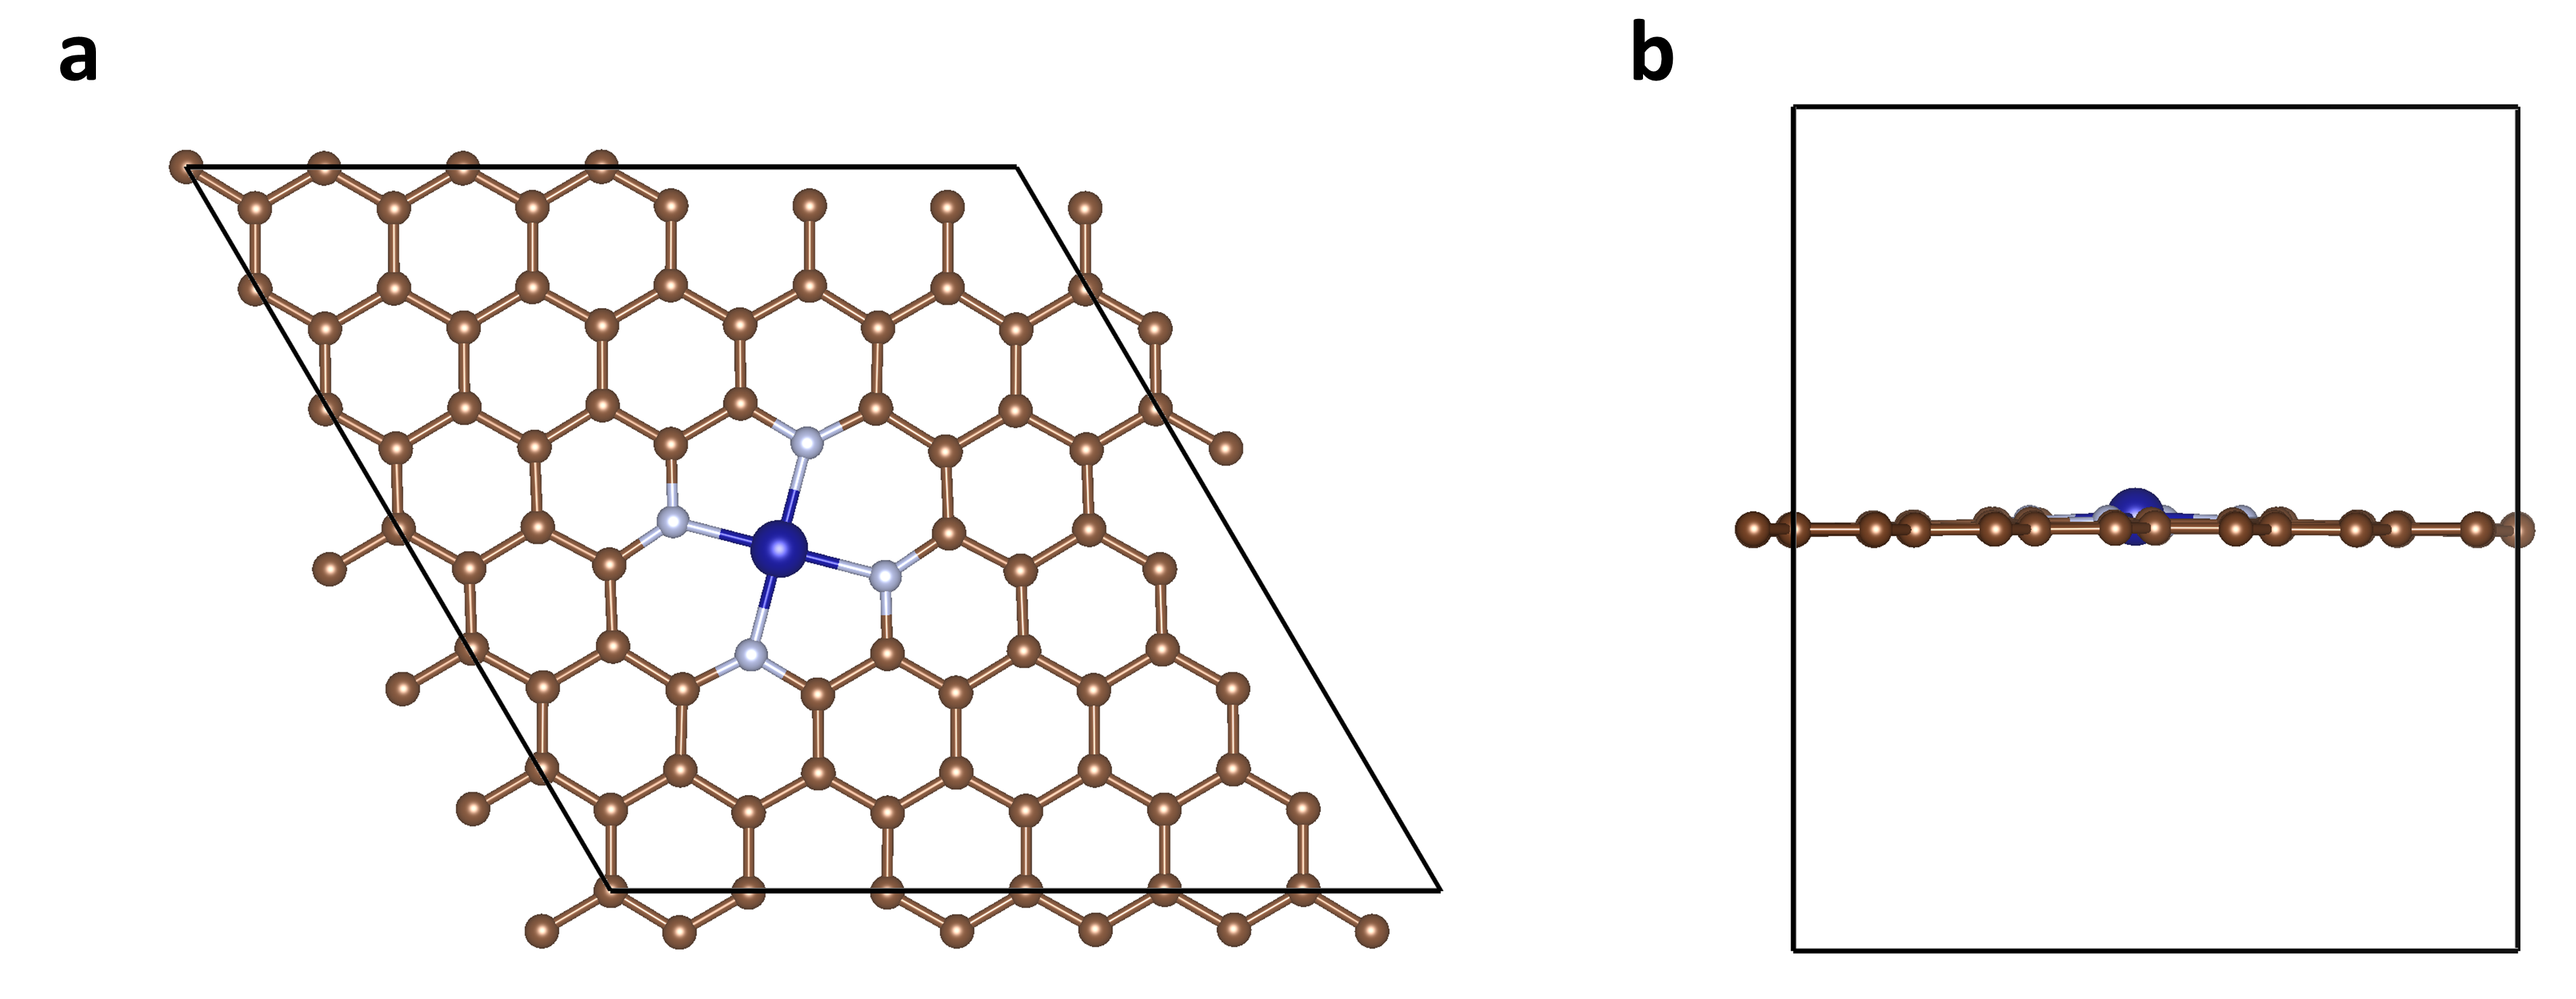
\includegraphics[width=\textwidth]{supp_fig3_Cr-n-gra.png}
  \caption{\textbf{Structure of single chromium atom supported on nitrogen-doped graphene.}
  (\textbf{a}) View along the z-axis and (\textbf{b}) view along the x-axis
  of the Cr@nitrogen-doped-graphene structure.
  In the illustrations, silver spheres represent N atoms, brown spheres
  signify C atoms, and indigo sphere indicates Cr atom.}
  \label{supp_fig3:Cr-n-gra}
\end{figure}

% SI Figure 4: Structure of Os atom supported on graphene with dual-vacancy
\begin{figure}[htbp]
  \centering
  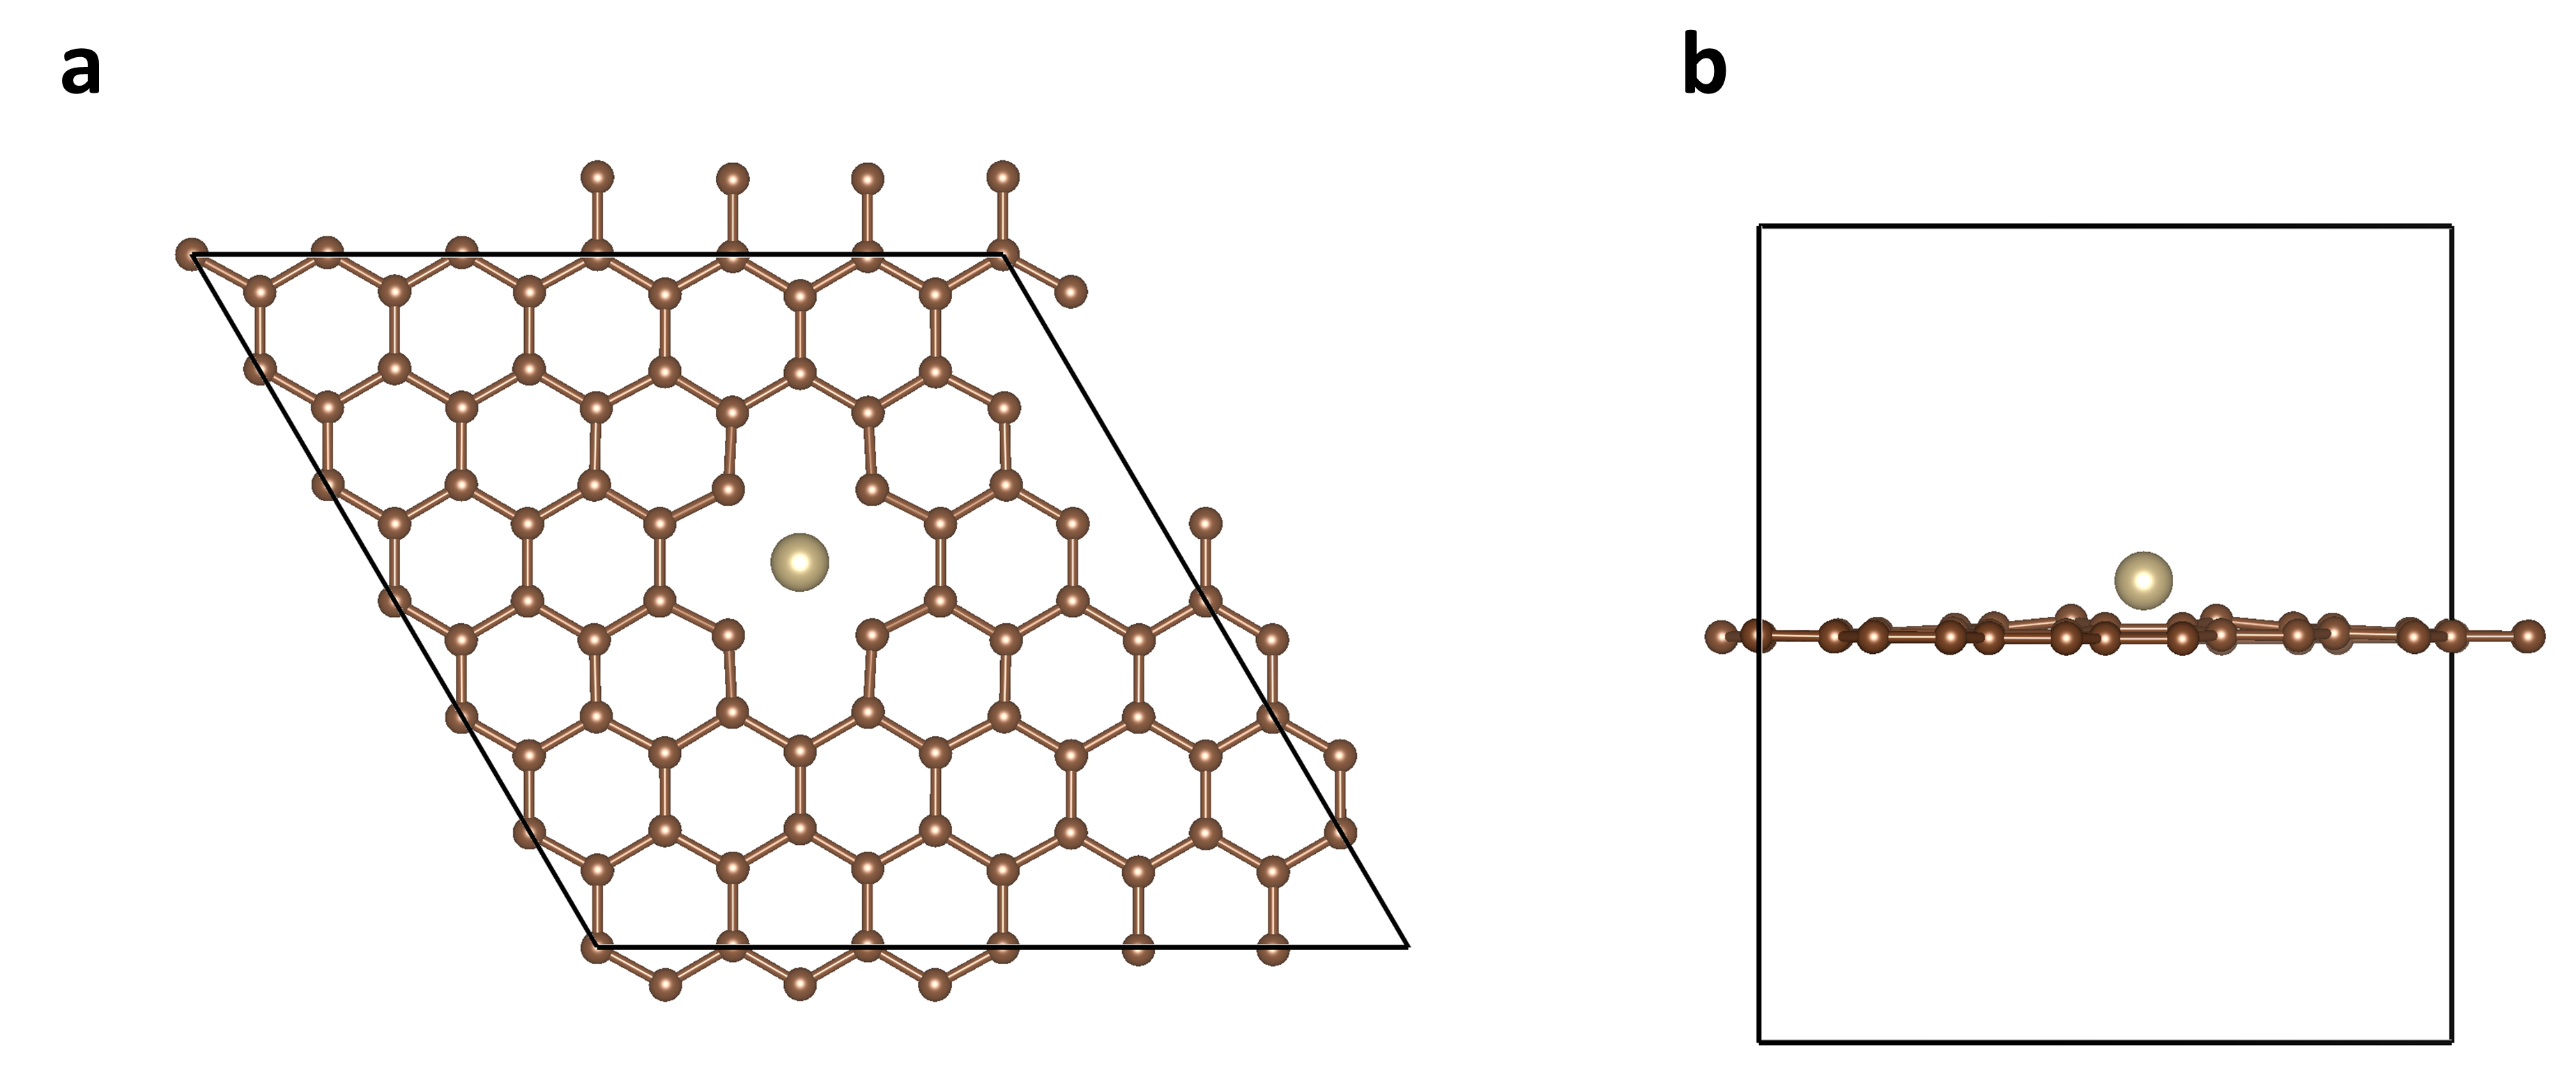
\includegraphics[width=\textwidth]{supp_fig4_Os-gra-vac.png}
  \caption{\textbf{Structure of single osmium atom supported on graphene with dual-vacancy.}
  (\textbf{a}) View along the z-axis and (\textbf{b}) view along the x-axis
  of the Os@graphene-with-dual-vacancy structure.
  In the illustrations, brown spheres signify C atoms, and light yellow sphere
  indicates Os atom.}
  \label{supp_fig4:Os-gra-vac}
\end{figure}

% SI Figure 5: Structure of Cr atom supported on black phosphorous
\begin{figure}[htbp]
  \centering
  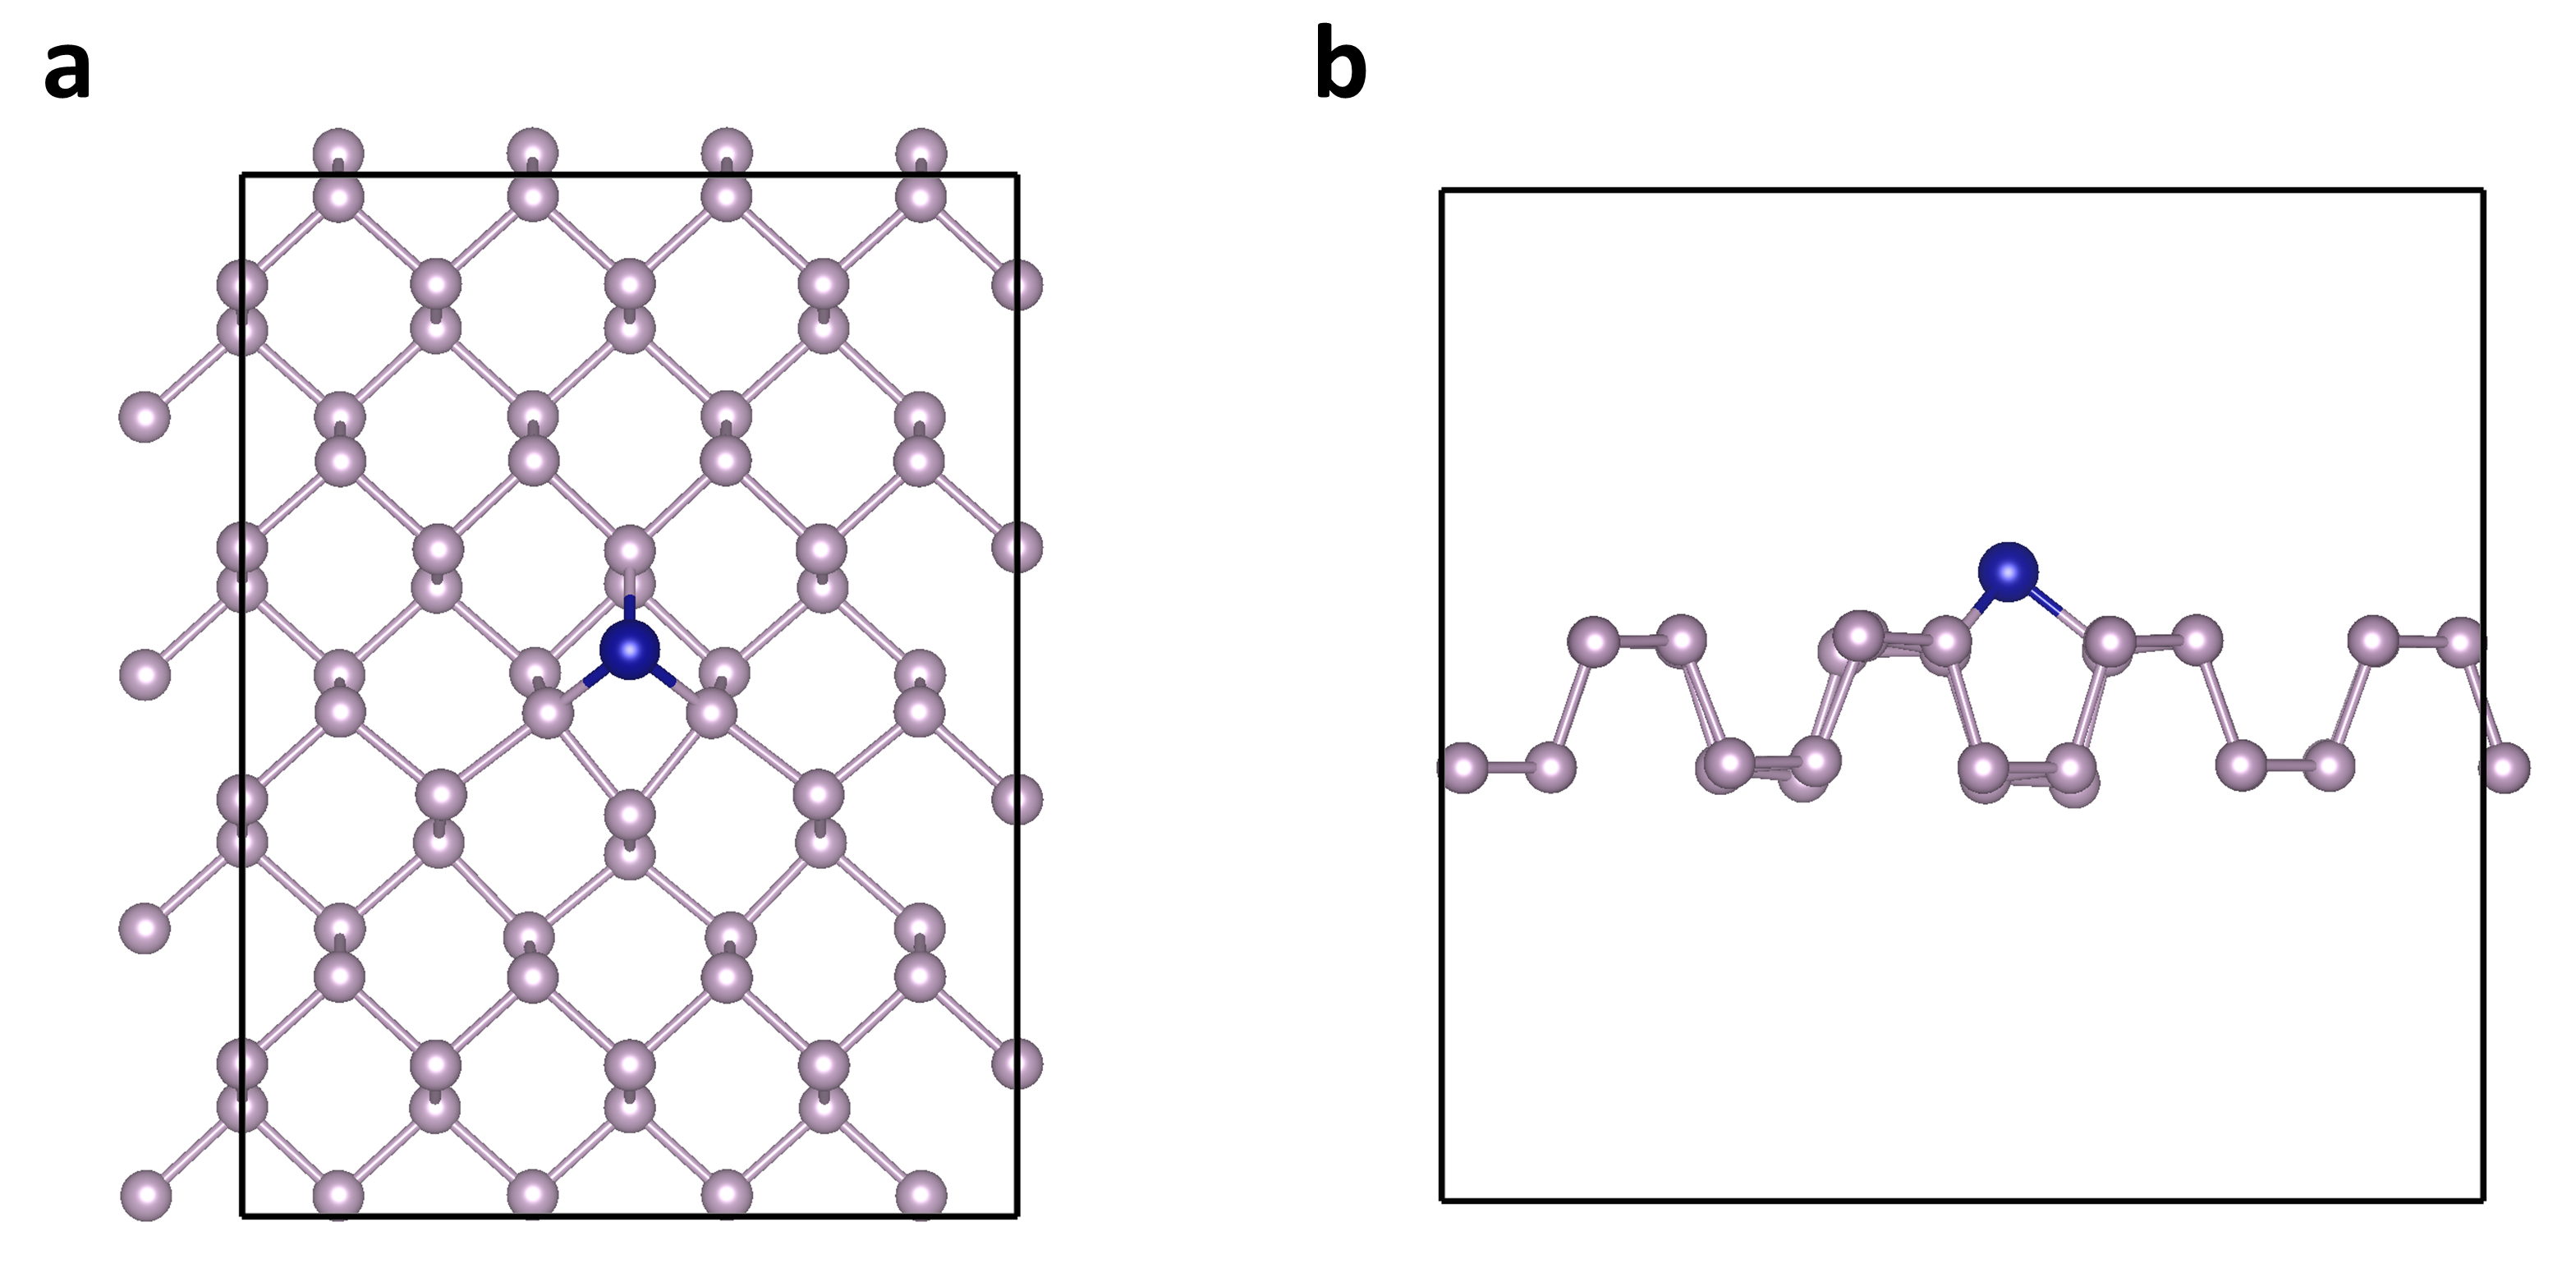
\includegraphics[width=\textwidth]{supp_fig5_Cr-BP.png}
  \caption{\textbf{Structure of single chromium atom supported on black phosphorous.}
  (\textbf{a}) View along the z-axis and (\textbf{b}) view along the x-axis
  of the Cr@black phosphorous structure.
  In the illustrations, light purple spheres represent P atoms, and indigo sphere
  indicates Cr atom.}
  \label{supp_fig5:Cr-BP}
\end{figure}

% SI Figure 6: Structure of Y atom supported on boron nitride
\begin{figure}[htbp]
  \centering
  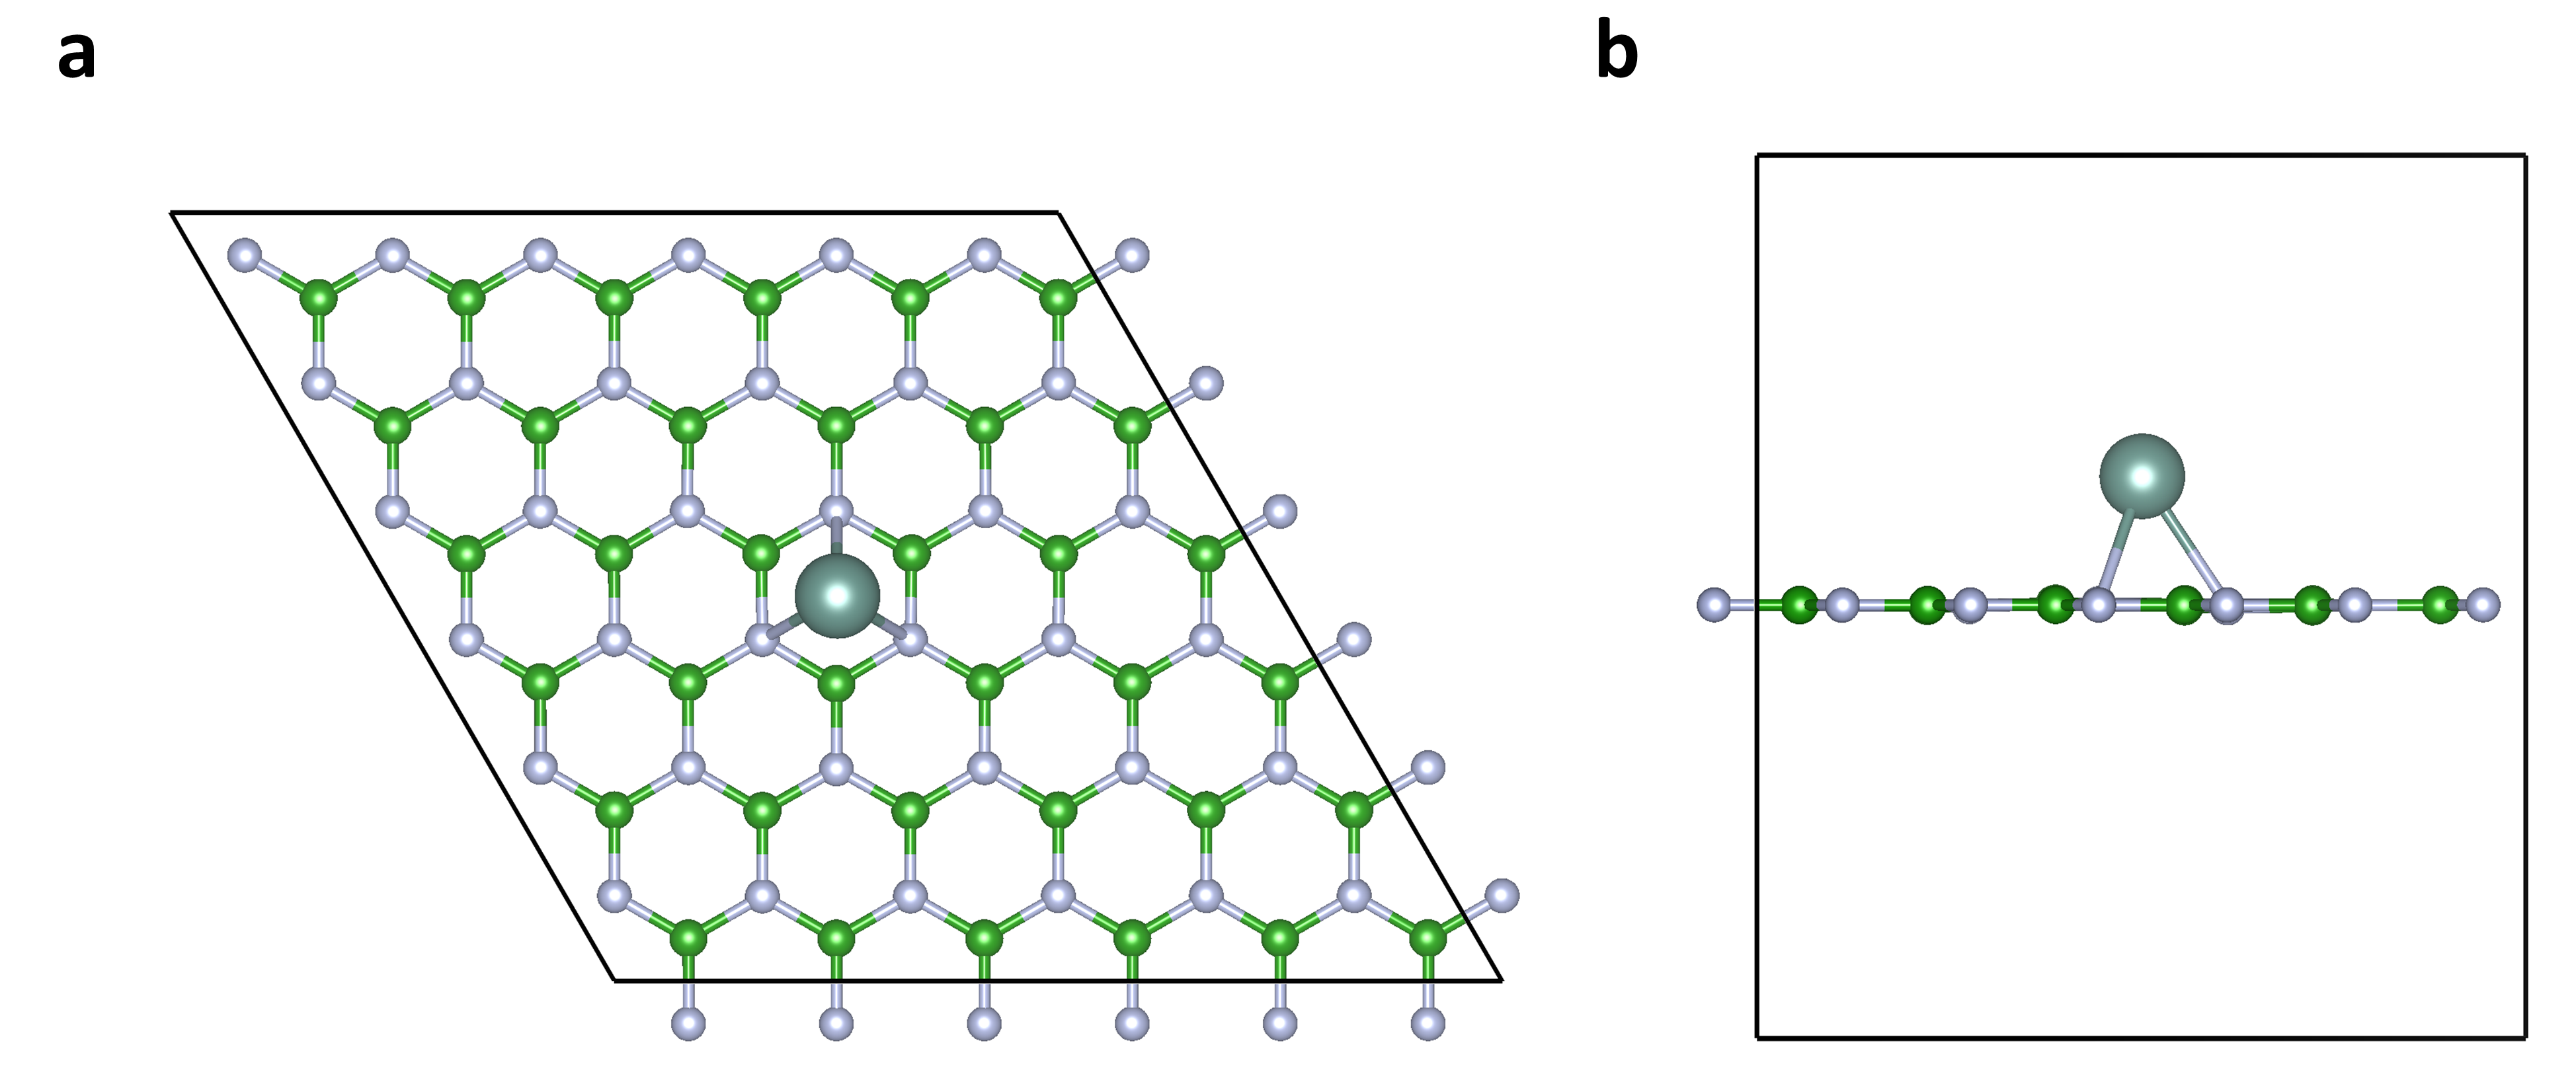
\includegraphics[width=\textwidth]{supp_fig6_Y-BN.png}
  \caption{\textbf{Structure of single yttrium atom supported on boron nitride.}
  (\textbf{a}) View along the z-axis and (\textbf{b}) view along the x-axis
  of the Y@boron-nitride structure.
  In the illustrations, silver spheres represent N atoms, green spheres
  signify B atoms, and light green sphere indicates Y atom.}
  \label{supp_fig6:Y-BN}
\end{figure}

% SI Figure 7: Structure of Al atom supported on C2N
\begin{figure}[htbp]
  \centering
  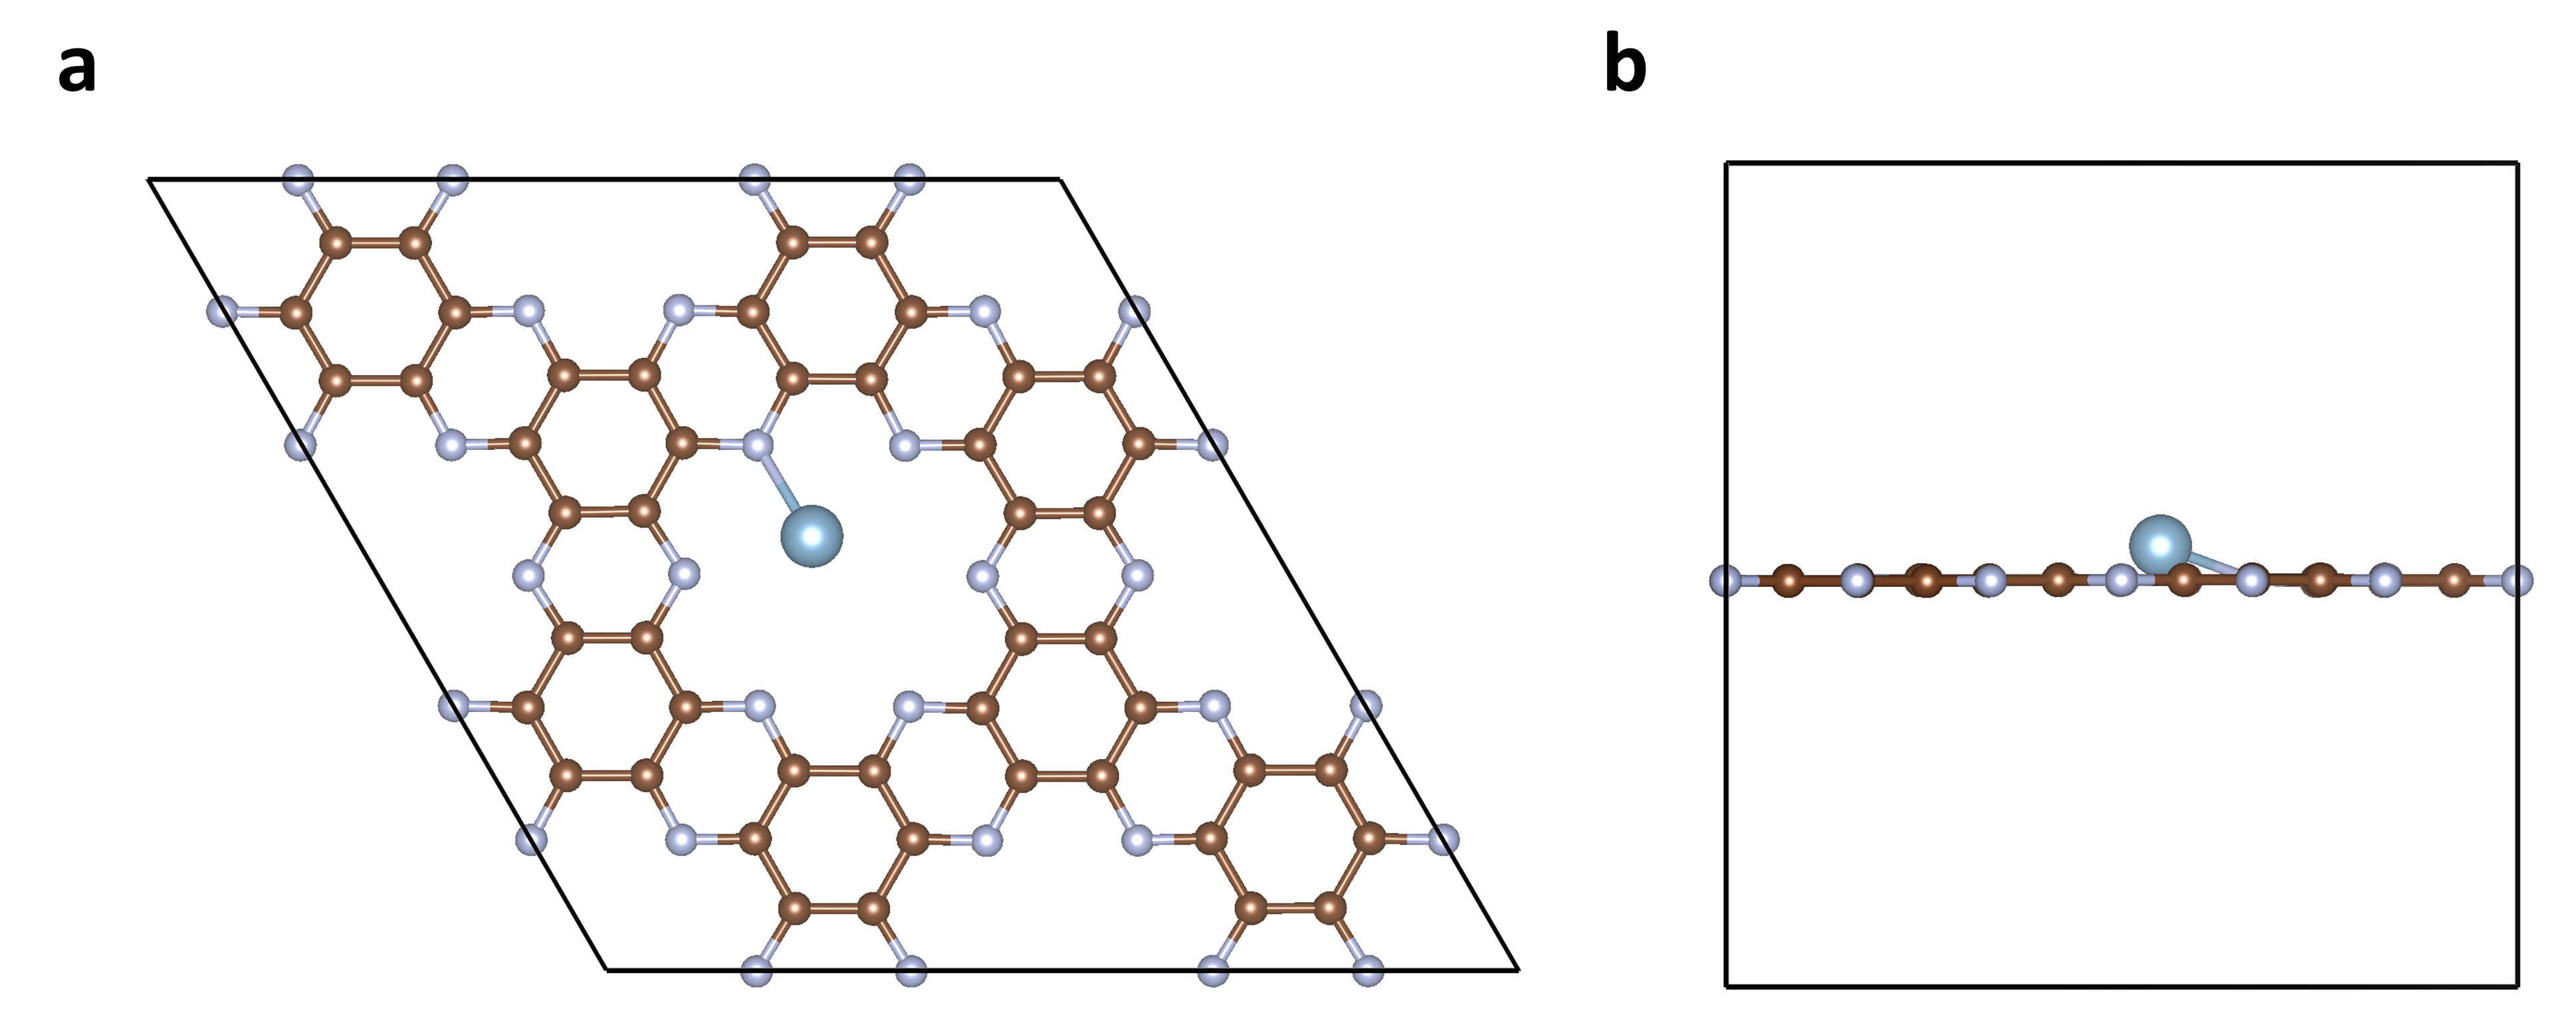
\includegraphics[width=\textwidth]{supp_fig7_Al-C2N.png}
  \caption{\textbf{Structure of single aluminum atom supported on C\textsubscript{2}N.}
  (\textbf{a}) View along the z-axis and (\textbf{b}) view along the x-axis
  of the Al@C\textsubscript{2}N structure.
  In the illustrations, silver spheres represent N atoms, brown spheres
  signify C atoms, and blue sphere indicates Al atom.}
  \label{supp_fig7:Al-C2N}
\end{figure}

\subsection{CO\textsubscript{2}RR pathways}
\label{supp_sec2.2_co2rr_paths}

In this study, we explored three reaction pathways that have been previously documented in the literature \cite{durand2011structure, nie2014reaction, peterson2010copper}, as depicted in \cref{supp_fig8:co2rr_paths}.
The adsorption configuration of the *CHO intermediate is pivotal in each of these pathways for determining the reaction mechanism in the CO\textsubscript{2}RR process.
We calculated the energies associated with the *CHO intermediate for catalysts
supported on g-C\textsubscript{3}N\textsubscript{4}, nitrogen-doped graphene, and dual-vacancy graphene-under each mechanism.
These calculations are summarized in \cref{supp_table1:e_3_co2rr_paths}.
Our results indicate that Pathway 1 is the most energetically favorable for most catalysts we investigated.
Therefore, to streamline our analysis, we focused exclusively on Mechanism 1 across all catalysts examined.

% SI Figure 8: Three investigated CO2RR pathways
\begin{figure}[htbp]
  \centering
  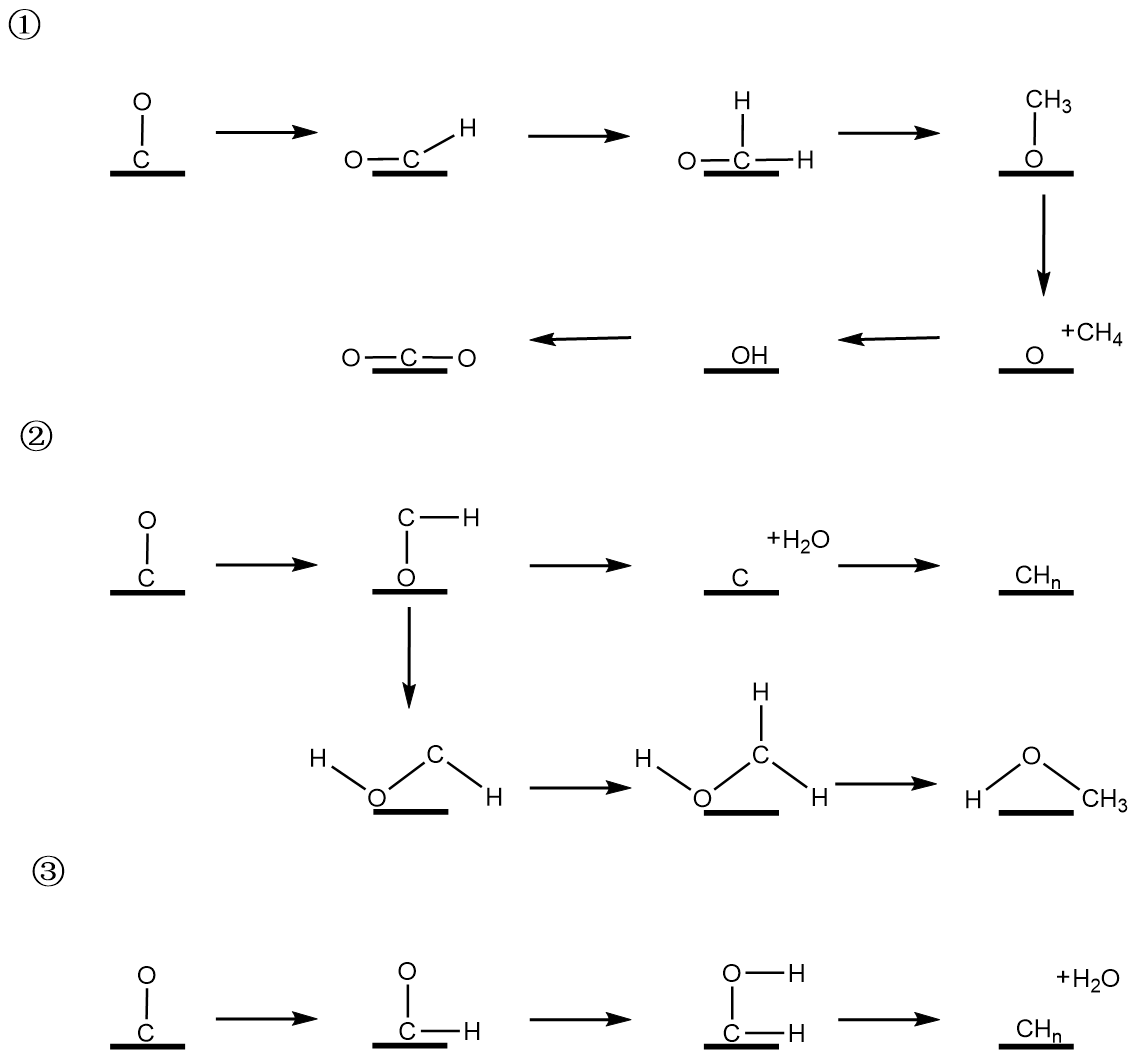
\includegraphics[width=0.8\textwidth]{supp_fig8_co2rr_paths.png}
  \caption{\textbf{Three investigated CO\textsubscript{2}RR pathways \cite{durand2011structure, nie2014reaction, peterson2010copper} investigated in this work.}}
  \label{supp_fig8:co2rr_paths}
\end{figure}

% Supplementary Table 1: DFT-calculated energies for protonated *CO intermediate for 3 pathways
\begin{table}[htbp]
\label{supp_table1:e_3_co2rr_paths}
  \caption{DFT-calculated energies in eV for protonated *CO intermediate
    for three investigated CO\textsubscript{2}RR pathways.}
  \resizebox{\textwidth}{!}{%
    \begin{tabular}{l *{9}{l}}
      \toprule
      \multirow{2}{*}{Metal}
      & \multicolumn{3}{c}{g-C\textsubscript{3}N\textsubscript{4}}
      & \multicolumn{3}{c}{nitrogen-doped graphene}
      & \multicolumn{3}{c}{graphene with dual-vacancy}  \\ \cline{2-10}
      & Pathway-1 & Pathway-2 & Pathway-3
      & Pathway-1 & Pathway-2 & Pathway-3
      & Pathway-1 & Pathway-2 & Pathway-3  \\
      \midrule
      Al & \textbf{-499.3494} & -497.8343 & -499.3005 & \textbf{-670.3489} & -668.5142 & -670.3093 & -667.2538 & -666.6725 & \textbf{-667.2665} \\
      Co & -502.5946 & -501.1257 & \textbf{-502.6139} & -672.8847 & -670.8013 & \textbf{-672.9020} & \textbf{-671.6284} & -670.4388 & -671.3827 \\
      Cr & -505.6012 & -504.2022 & \textbf{-505.6029} & -675.3126 & -674.1640 & \textbf{-675.3480} & \textbf{-673.4283} & -672.1919 & -673.3818 \\
      Cu & \textbf{-495.8913} & -493.6853 & -495.8820 & \textbf{-666.9894} & -664.9810 & -666.9705 & -666.9876 & -664.7684 & \textbf{-667.1395} \\
      Fe & \textbf{-501.3325} & -499.3969 & -501.3221 & -673.8242 & -672.0887 & \textbf{-673.8478} & \textbf{-672.7810} & -671.5694 & -672.4960 \\
      Ga & -498.2365 & -496.3967 & \textbf{-498.2912} & \textbf{-667.3963} & -665.4677 & -667.3482 & -665.7780 & -664.8573 & \textbf{-665.8030} \\
      Ge & -500.2052 & -497.9780 & \textbf{-500.2156} & \textbf{-668.1785} & -666.3484 & -668.1463 & \textbf{-667.7387} & -665.7394 & -667.7324 \\
      Mn & \textbf{-502.6355} & -500.8006 & -502.6294 & -674.6848 & -672.9574 & \textbf{-674.7030} & -673.2243 & -672.6495 & \textbf{-673.2361} \\
      Ni & \textbf{-500.4085} & -498.5165 & -500.3985 & \textbf{-670.0979} & -667.9544 & -670.0832 & -670.1619 & -668.3684 & \textbf{-670.1756} \\
      Sc & -503.4428 & -501.6129 & \textbf{-503.4437} & \textbf{-673.9590} & -671.7624 & -673.3818 & \textbf{-670.0841} & -668.1044 & -669.6050 \\
      Ti & -503.7848 & -502.6148 & \textbf{-503.8033} & \textbf{-675.1006} & -673.2417 & -674.6257 & \textbf{-672.7127} & -670.6787 & -672.2491 \\
      V  & \textbf{-503.6115} & -502.6188 & -503.5956 & \textbf{-675.0533} & -674.0394 & -675.0136 & \textbf{-673.1855} & -671.5382 & -673.1583 \\
      Zn & \textbf{-493.9854} & -491.5010 & -493.9743 & \textbf{-664.9935} & -663.0932 & -664.9758 & -663.7735 & -661.8097 & \textbf{-663.7959} \\
      Ag & \textbf{-494.4055} & -492.4511 & -494.3905 & -664.6322 & -662.9060 & \textbf{-664.6353} & -664.3972 & -662.3588 & \textbf{-665.0570} \\
      Cd & \textbf{-493.3084} & -491.1781 & -493.2951 & \textbf{-663.8832} & -661.6272 & -663.8653 & -661.8518 & -659.9601 & \textbf{-661.8631} \\
      In & -498.5272 & -496.6593 & \textbf{-498.5908} & \textbf{-666.3968} & -663.7707 & -666.3845 & -663.6532 & -661.5581 & \textbf{-663.6913} \\
      Mo & \textbf{-504.5248} & -503.3763 & -504.5148 & -675.3472 & -674.7118 & \textbf{-675.4389} & -674.7186 & -672.9335 & \textbf{-674.7397} \\
      Nb & -505.3967 & -504.7113 & \textbf{-505.3982} & \textbf{-676.0492} & -674.1997 & -675.4107 & \textbf{-674.6606} & -672.8268 & -674.5488 \\
      Pd & -500.0370 & -498.3310 & \textbf{-500.0455} & \textbf{-669.0243} & -667.0759 & -669.0205 & \textbf{-669.1169} & -667.3223 & -669.1119 \\
      Rh & \textbf{-499.2225} & -497.3162 & -499.2170 & -672.7920 & -670.7853 & \textbf{-672.8099} & \textbf{-671.4286} & -670.3036 & -671.4181 \\
      Ru & \textbf{-503.9986} & -502.1908 & -503.9640 & -674.0273 & -672.4060 & \textbf{-674.0339} & \textbf{-672.9956} & -672.1332 & -672.9909 \\
      Sb & \textbf{-497.3836} & -495.1348 & -497.3442 & \textbf{-666.7198} & -664.9611 & -666.7190 & -666.8632 & -664.8131 & \textbf{-666.8670} \\
      Sn & \textbf{-499.4952} & -497.2007 & -499.1116 & \textbf{-667.1459} & -665.3835 & -667.0999 & \textbf{-665.9821} & -663.8277 & -665.9755 \\
      Tc & \textbf{-503.0602} & -501.1754 & -503.0532 & -674.4342 & -673.8164 & \textbf{-674.4559} & -674.0615 & -672.9747 & \textbf{-674.0738} \\
      Y  & \textbf{-503.9232} & -502.0670 & -503.8988 & \textbf{-673.7620} & -671.6132 & -673.2241 & -669.4633 & -668.0403 & \textbf{-669.5030} \\
      Zr & \textbf{-505.2907} & -503.9148 & -505.1817 & \textbf{-675.6874} & -673.5456 & -675.0519 & \textbf{-673.1694} & -671.1993 & -672.8072 \\
      Au & \textbf{-497.0784} & -495.1720 & -497.0175 & \textbf{-665.1479} & -663.3239 & -665.1370 & -666.4185 & -664.2892 & \textbf{-666.5182} \\
      Bi & \textbf{-496.9946} & -494.7679 & -496.9934 & -665.9563 & -664.2409 & \textbf{-666.0512} & \textbf{-665.0896} & -663.2974 & -665.0887 \\
      Hf & \textbf{-506.4837} & -504.9734 & -506.4777 & \textbf{-677.3077} & -675.1797 & -676.6502 & \textbf{-674.7209} & -672.6650 & -674.2149 \\
      Hg & \textbf{-491.0035} & -488.7951 & -490.9728 & \textbf{-661.2458} & -659.2406 & -661.2398 & -661.7192 & -659.8398 & \textbf{-661.7300} \\
      Ir & \textbf{-503.0227} & -501.1368 & -503.0217 & -673.9926 & -672.0068 & \textbf{-674.0087} & \textbf{-673.5129} & -672.6725 & -673.4975 \\
      Os & -504.7648 & -502.9878 & \textbf{-504.8105} & -675.2098 & -673.6653 & \textbf{-675.2235} & \textbf{-674.9483} & -674.1970 & -674.9223 \\
      Pb & \textbf{-499.1183} & -497.1173 & -499.0544 & -666.4446 & -664.6897 & \textbf{-666.4625} & \textbf{-664.0200} & -662.2222 & -664.0123 \\
      Pt & \textbf{-499.3356} & -497.5110 & -499.3215 & -670.3996 & -668.2412 & \textbf{-670.4147} & \textbf{-671.1408} & -669.2725 & -671.1370 \\
      Re & \textbf{-504.1830} & -502.4735 & -504.1746 & \textbf{-675.7670} & -675.0715 & -675.7486 & \textbf{-675.8701} & -674.9245 & -675.8233 \\
      Ta & -506.6180 & -505.7793 & \textbf{-506.6241} & \textbf{-677.7222} & -675.9907 & -677.0911 & \textbf{-676.4371} & -674.5434 & -676.4262 \\
      Tl & \textbf{-497.9559} & -496.1578 & -497.9382 & -664.5047 & -662.7051 & \textbf{-664.5051} & -662.6279 & -660.6086 & \textbf{-662.6317}\\
      W  & \textbf{-505.8134} & -504.9085 & -505.8030 & -676.5304 & -676.1384 & \textbf{-676.9965} & \textbf{-676.7669} & -675.4895 & -676.7356 \\
      \bottomrule
    \end{tabular}
  }

  \smallskip

  \footnotesize\textit{Note:} Energies of the most stable configurations are highlighted in bold.
\end{table}

\subsection{DFT energies and energy corrections}
\label{supp_sec2.3_energies}

% Supplementary Table 2: Free energies for isolated species.
\begin{table}[htbp]
\label{supp_table2:species_free_energies}
  \caption{Free energies at 298.15 K for isolated species.}
  \small
  \begin{tabularx}{\textwidth}{@{}lXr@{}}
    \toprule
    Species               & Free Energy (eV)  \\
    \midrule
    CO\textsubscript{2}   & -23.3140          \\
    CO                    & -15.3336          \\
    CH\textsubscript{4}   & -23.4639          \\
    H\textsubscript{2}    & -6.9315           \\
    H\textsubscript{2}O   & -14.3239          \\
    COOH                  & -24.3963          \\
    CHO                   & -17.0983          \\
    CH\textsubscript{2}O  & -22.1607          \\
    OCH\textsubscript{3}  & -24.5075          \\
    O                     & -1.9007           \\
    OH                    & -7.7303           \\
    \bottomrule
  \end{tabularx}

  \smallskip

  \footnotesize\textit{Note:} VASPKIT \cite{wang2021vaspkit} was employed to calculate free energies.
\end{table}

% Supplementary Table 3: Free energy corrections for adsorbed intermediates
\begin{table}[htbp]
\label{supp_table3:ads_e_correction}
  \caption{Free energy corrections at 298.15 K for adsorbed intermediates.}
  \small
  \begin{tabularx}{\textwidth}{@{}lXr@{}}
    \toprule
    Species                & Free energy correction (eV)  \\
    \midrule
    *CO\textsubscript{2}   &  0.0864                      \\
    *COOH                  &  0.3693                      \\
    *CO                    &  0.0111                      \\
    *CHO                   &  0.2716                      \\
    *CH\textsubscript{2}O  &  0.5595                      \\
    *OCH\textsubscript{3}  &  0.8738                      \\
    *O                     & -0.0193                      \\
    *OH                    &  0.1993                      \\
    *H                     &  0.1533                      \\
    \bottomrule
  \end{tabularx}

  \smallskip

  \footnotesize\textit{Note:} {Free energy corrections were obtained by averaging the
  DFT-computed corrections, which include zero-point energy and entropy, across three substrates:
  g-C\textsubscript{3}N\textsubscript{4}, nitrogen-doped graphene, and dual-vacancy graphene.}
\end{table}

% Supplementary Table 4: DFT calculated final state energies for adsorbates supported on g-c3n4
\begin{table}[htbp]
\label{supp_table4:e_g-c3n4}
  \caption{DFT calculated final state energies in eV for adsorbates
    supported on g-C\textsubscript{3}N\textsubscript{4}.}
  \resizebox{\textwidth}{!}{%
    \begin{tabular}{l *{9}{l}}
      \toprule
      Metal & *CO\textsubscript{2} & *COOH    & *CO       & *CHO
      & *CH\textsubscript{2}O  & *OCH\textsubscript{3}  & *O        & *OH       & *H        \\
      \midrule
      Al & -481.2292 & -504.7972 & -508.6897 & -496.4490 & -500.7640 & -503.7935 & -509.9998 & -488.6623 & -485.4855 \\
      Co & -483.2039 & -507.0765 & -510.0453 & -500.1329 & -503.9316 & -507.0552 & -510.9052 & -489.9487 & -486.6194 \\
      Cr & -486.7813 & -509.9599 & -513.3962 & -502.1493 & -505.7125 & -509.8851 & -514.1702 & -493.7457 & -489.9202 \\
      Cu & -477.5955 & -502.5914 & -505.9613 & -495.6511 & -498.0502 & -502.4590 & -506.2829 & -484.3166 & -481.9683 \\
      Fe & -482.0576 & -507.1508 & -510.2918 & -500.1101 & -502.1626 & -506.0115 & -511.2543 & -490.0116 & -486.4067 \\
      Ga & -480.8854 & -503.9317 & -506.4938 & -495.7379 & -498.7813 & -503.1345 & -507.5029 & -486.1702 & -483.4575 \\
      Ge & -481.5807 & -504.6467 & -508.4204 & -496.4421 & -500.5712 & -504.0218 & -509.4116 & -488.4168 & -485.2680 \\
      Mn & -483.7690 & -508.5410 & -511.6514 & -500.6279 & -502.6739 & -508.6433 & -512.8569 & -491.2239 & -488.1082 \\
      Ni & -482.0061 & -505.1988 & -508.4173 & -498.5054 & -501.0040 & -504.8945 & -508.6266 & -487.3684 & -484.8272 \\
      Sc & -483.9963 & -509.3147 & -512.9882 & -501.4505 & -505.2024 & -509.4054 & -514.5969 & -493.4105 & -489.2632 \\
      Ti & -484.2282 & -509.6510 & -512.8528 & -502.0410 & -505.3761 & -509.9729 & -514.0700 & -493.6478 & -489.2234 \\
      V  & -484.1990 & -508.6926 & -512.3009 & -501.6777 & -504.4297 & -509.3618 & -513.4561 & -493.8569 & -488.9474 \\
      Zn & -475.2375 & -500.3556 & -504.4103 & -492.4144 & -496.5426 & -499.4232 & -504.6297 & -482.6782 & -481.0438 \\
      Ag & -476.7049 & -501.6430 & -504.5861 & -493.9138 & -496.7220 & -500.9477 & -504.5408 & -482.6604 & -481.2659 \\
      Cd & -475.1288 & -500.1854 & -503.4108 & -491.8954 & -495.6486 & -499.4959 & -503.6209 & -483.3427 & -479.8278 \\
      In & -481.1330 & -504.1653 & -506.4422 & -496.0016 & -498.6643 & -503.3286 & -507.3780 & -485.6281 & -483.1445 \\
      Mo & -484.2892 & -509.4263 & -512.9103 & -503.0025 & -505.5534 & -509.6730 & -513.0136 & -493.5700 & -489.4994 \\
      Nb & -485.4055 & -510.7952 & -514.0380 & -503.5663 & -506.3671 & -511.1572 & -514.7845 & -495.5118 & -490.2111 \\
      Pd & -481.5399 & -504.7593 & -508.5173 & -498.0817 & -501.1620 & -504.0892 & -508.1976 & -486.1551 & -483.9553 \\
      Rh & -479.8884 & -505.2422 & -508.6754 & -498.7129 & -501.4594 & -504.5254 & -508.9536 & -487.8771 & -485.0738 \\
      Ru & -483.8526 & -507.5120 & -511.5881 & -500.6857 & -504.1497 & -506.8934 & -510.9524 & -490.6690 & -488.0169 \\
      Sb & -478.5169 & -502.9708 & -506.5211 & -494.8740 & -498.9453 & -502.5347 & -507.2111 & -486.4448 & -483.4418 \\
      Sn & -481.4238 & -504.4677 & -507.8470 & -496.2883 & -499.9258 & -503.6685 & -508.8152 & -487.6963 & -484.6351 \\
      Tc & -482.7091 & -507.9652 & -512.1064 & -501.9896 & -504.6034 & -508.3486 & -511.4777 & -492.0381 & -488.0897 \\
      Y  & -484.6612 & -509.8564 & -513.6851 & -501.9522 & -505.8238 & -509.8344 & -515.2400 & -493.4038 & -489.6506 \\
      Zr & -485.4694 & -511.1852 & -514.3901 & -503.1958 & -506.9346 & -511.5864 & -515.6720 & -496.3037 & -490.4785 \\
      Au & -479.1941 & -502.3245 & -506.9013 & -495.6782 & -499.0711 & -501.6877 & -506.5462 & -484.6198 & -483.6909 \\
      Bi & -478.2695 & -502.8490 & -506.2055 & -494.6965 & -498.5557 & -502.3398 & -506.7999 & -485.7536 & -483.1348 \\
      Hf & -486.5155 & -512.4535 & -515.5965 & -504.3393 & -508.1599 & -512.8332 & -517.2187 & -496.4195 & -491.7486 \\
      Hg & -472.8730 & -500.0491 & -502.1889 & -491.7544 & -494.1224 & -499.2181 & -501.8365 & -480.3761 & -479.2046 \\
      Ir & -483.7878 & -507.2024 & -510.6763 & -500.2051 & -503.2948 & -506.5209 & -509.8509 & -490.9790 & -487.3503 \\
      Os & -484.9279 & -508.6427 & -512.5954 & -501.8541 & -505.2080 & -507.8334 & -511.8734 & -491.0155 & -489.0898 \\
      Pb & -481.3587 & -504.4450 & -507.5634 & -496.2379 & -499.6114 & -503.5822 & -508.1698 & -486.8476 & -484.2646 \\
      Pt & -481.1676 & -504.3670 & -508.2170 & -499.0073 & -500.9446 & -504.2695 & -508.1465 & -487.3508 & -484.6644 \\
      Re & -483.6421 & -508.9474 & -512.8388 & -502.8952 & -505.3651 & -509.1168 & -512.6374 & -493.0621 & -489.2811 \\
      Ta & -486.3299 & -512.1371 & -515.1895 & -504.6585 & -507.5888 & -512.5295 & -516.0165 & -497.0134 & -490.5695 \\
      Tl & -480.7357 & -503.7632 & -505.9937 & -495.5894 & -497.7724 & -503.0564 & -506.7919 & -484.0732 & -482.3846 \\
      W  & -485.2596 & -510.8145 & -514.28   & -504.2714 & -506.7988 & -511.0643 & -514.2358 & -494.4330 & -490.6506 \\
      \bottomrule
    \end{tabular}
  }
\end{table}

% Supplementary Table 5: DFT calculated final state energies for adsorbates supported on n-doped graphene
\begin{table}[htbp]
\label{supp_table5:e_n_gra}
    \caption{DFT calculated final state energies in eV for adsorbates supported on nitrogen-doped graphene.}
    \resizebox{\textwidth}{!}{%
      \begin{tabular}{l *{9}{l}}
        \toprule
        Metal & *CO\textsubscript{2} & *COOH    & *CO       & *CHO
        & *CH\textsubscript{2}O  & *OCH\textsubscript{3}  & *O        & *OH       & *H        \\
        \midrule
        Al	& -652.7589	&-675.7997	&-679.7595	&-668.0296	&-671.7596	&-676.2161	&-681.1311	&-658.7849	&-656.4702 \\
        Co	& -654.3280 &-677.5394	&-681.2518	&-670.0860  &-673.9208	&-676.7761	&-680.7219	&-659.1714	&-657.8777 \\
        Cr	& -657.0479	&-680.2074	&-683.7982	&-673.0760  &-676.1859	&-679.4701	&-684.5295	&-664.7306	&-660.4141 \\
        Cu	& -650.2181	&-673.3928	&-675.5873	&-665.2174	&-668.0662	&-672.5797	&-675.7047	&-653.5770  &-652.1010 \\
        Fe	& -655.4034	&-678.5897	&-682.1186	&-671.9101	&-674.7438	&-677.8515	&-682.1216	&-661.5422	&-658.7383 \\
        Ga	& -649.9563	&-672.9807	&-676.9763	&-664.9727	&-669.0739	&-672.8536	&-677.7169	&-655.5345	&-653.9243 \\
        Ge	& -651.0391	&-674.1655	&-677.2582	&-665.9255	&-669.5282	&-673.3438	&-678.1585	&-657.4964	&-654.3444 \\
        Mn	& -656.5635	&-679.7128	&-683.1092	&-672.6753	&-675.6877	&-679.0710  &-683.3898	&-663.1584	&-659.7760 \\
        Ni	& -653.1461	&-676.3270  &-678.5166	&-668.1448	&-671.1502	&-675.5454	&-678.5411	&-656.3929	&-655.1238 \\
        Sc	& -655.2274	&-678.9985	&-682.8810  &-670.9489	&-674.9850  &-679.1986	&-684.3192	&-662.2442	&-659.0243 \\
        Ti	& -655.5937	&-680.2412	&-683.5514	&-671.9689	&-675.9724	&-680.4589	&-685.1366	&-665.2871	&-659.7132 \\
        V	  & -656.0751	&-680.2584	&-683.5739	&-672.6281	&-676.0229	&-680.5926	&-684.9400	&-665.6038	&-659.9017 \\
        Zn	& -648.2316	&-671.3824	&-674.1973	&-663.2623	&-666.3990 	&-670.5613	&-674.5436	&-652.2900  &-650.9227 \\
        Ag	& -646.9759	&-670.2666	&-673.2766	&-663.1058	&-665.7601	&-669.7801	&-673.0113	&-651.0760  &-649.9287 \\
        Cd	& -646.1687	&-669.2620  &-672.8043	&-661.4439	&-664.9473	&-668.8180  &-672.9588	&-650.7684	&-649.7670 \\
        In	& -648.6726	&-671.7218	&-675.3788	&-663.4885	&-667.5183	&-670.7536	&-675.8630  &-653.8535	&-652.4757 \\
        Mo	& -655.7944	&-680.2966	&-683.6262	&-672.7667	&-676.3955	&-680.6291	&-684.8234	&-665.8138	&-659.8169 \\
        Nb	& -656.0277	&-680.8814	&-684.2662	&-672.5576	&-676.9139	&-681.4203	&-685.7720  &-666.2363	&-660.3734 \\
        Pd	& -652.2091	&-675.3967	&-677.2760  &-667.1855	&-669.8609	&-674.6033	&-677.3498	&-655.1080  &-654.0027 \\
        Rh	& -653.6928	&-676.9529	&-680.9755	&-669.5137	&-673.6394	&-676.2879	&-680.2104	&-658.6953	&-657.6908 \\
        Ru	& -654.5425	&-678.2124	&-681.9561	&-672.0589	&-674.6177	&-678.0945	&-681.9008	&-661.3838	&-658.6572 \\
        Sb	& -649.9262	&-672.9182	&-675.6457	&-664.7128	&-667.9159	&-672.0849	&-675.8420 	&-655.1699	&-652.4240 \\
        Sn	& -650.5072	&-673.6118	&-675.7767	&-665.3842	&-668.0544	&-672.7597	&-676.5046	&-655.8947	&-652.9261 \\
        Tc	& -655.4025	&-679.3044	&-682.7454	&-672.5785	&-676.3294	&-679.4840  &-683.3209	&-664.2323	&-659.2703 \\
        Y	  & -655.2660 &-679.0430	&-682.7571	&-670.8208	&-674.7780  &-679.0775	&-684.1210  &-661.8034	&-658.8885 \\
        Zr	& -655.9118	&-680.6859	&-684.1920  &-672.1497	&-676.4014	&-680.7930  &-685.7940  &-665.4878	&-660.4163 \\
        Au	& -648.3344	&-671.3969	&-673.1469	&-663.1955	&-665.5964	&-670.5800	&-673.6092	&-651.2436	&-649.7275 \\
        Bi	& -649.1484	&-672.1225	&-675.1630  &-663.9594	&-667.2981	&-671.4617	&-675.6926	&-654.7684	&-651.8907 \\
        Hf	& -657.3364	&-682.3019	&-685.8119	&-673.6603	&-678.0090  &-682.4001	&-687.4607	&-666.9550  &-662.0651 \\
        Hg	& -644.7368	&-667.9224	&-671.2200	&-659.6906	&-663.5208	&-667.0466	&-670.9016	&-648.8944	&-648.3755 \\
        Ir	& -654.8564	&-678.1079	&-682.2865	&-670.9826	&-674.9484	&-677.4097	&-681.3088	&-660.1543	&-658.9895 \\
        Os	& -655.6722	&-679.5364	&-683.3240  &-673.4289	&-675.9254	&-679.4423	&-683.1300	&-663.0791	&-659.9901 \\
        Pb	& -649.8843	&-672.9588	&-674.5856	&-664.7553	&-667.1174	&-672.0886	&-675.8823	&-653.6827	&-651.5940 \\
        Pt	& -653.3281	&-676.5221	&-678.6094	&-668.2951	&-671.2463	&-675.7317	&-678.4334	&-656.4419	&-655.4733 \\
        Re	& -656.3492	&-680.7664	&-683.9596	&-673.9732	&-676.5164	&-681.0627	&-684.8096	&-665.9526	&-660.5620 \\
        Ta	& -657.1988	&-682.6048	&-685.8231	&-674.1666	&-678.5029	&-682.9709	&-687.2294	&-667.7321	&-661.8794 \\
        Tl	& -648.1346	&-671.1831	&-673.2953	&-662.9610  &-665.6240  &-670.3512	&-673.4567	&-651.7909	&-650.4750 \\
        W	  & -657.0204	&-682.0186	&-685.3735	&-674.3843	&-678.2483	&-682.4377	&-686.3613	&-667.4547	&-661.5686 \\
        \bottomrule
      \end{tabular}
    }
\end{table}

% Supplementary Table 6: DFT calculated final state energies for adsorbates supported on graphene with dual-vac
\begin{table}[htbp]
\label{supp_table6:e_vac_gra}
  \caption{DFT calculated final state energies in eV for adsorbates supported on graphene with dual-vacancy.}
  \resizebox{\textwidth}{!}{%
    \begin{tabular}{l *{9}{c}}
      \toprule
      Metal & *CO\textsubscript{2} & *COOH    & *CO       & *CHO
      & *CH\textsubscript{2}O  & *OCH\textsubscript{3}  & *O        & *OH       & *H        \\
      \midrule
      Al & -650.3496 & -673.3468 & -676.2273 & -665.6303 & -668.4112 & -672.5763 & -677.4453 & -655.0864 & -653.0166 \\
      Co & -652.5157 & -675.5864 & -679.3861 & -669.0614 & -672.8955 & -675.8508 & -679.5268 & -658.7929 & -655.9377 \\
      Cr & -655.0421 & -678.1256 & -681.8470 & -671.1282 & -674.2868 & -679.1554 & -683.4111 & -663.3554 & -658.4913 \\
      Cu & -649.8187 & -672.9161 & -674.9327 & -664.8190 & -669.0819 & -672.1515 & -674.7438 & -652.8789 & -653.6953 \\
      Fe & -653.7964 & -677.0127 & -680.3412 & -670.0219 & -673.9525 & -676.7631 & -681.1346 & -660.9239 & -656.9759 \\
      Ga & -649.0340 & -672.0433 & -674.9630 & -663.8505 & -667.2101 & -671.2541 & -675.5229 & -653.2086 & -651.8693 \\
      Ge & -651.0133 & -674.2532 & -677.2272 & -666.0554 & -669.5660 & -673.4485 & -677.8152 & -655.7843 & -654.2731 \\
      Mn & -654.8183 & -678.0584 & -681.5834 & -670.9593 & -674.0994 & -677.9260 & -682.6048 & -662.5702 & -658.1064 \\
      Ni & -651.5295 & -674.6692 & -677.8941 & -667.2937 & -670.7325 & -673.9392 & -677.5204 & -656.1026 & -655.6559 \\
      Sc & -652.1630 & -675.5777 & -678.6101 & -667.5024 & -670.7255 & -675.4361 & -680.0287 & -658.0834 & -654.6913 \\
      Ti & -654.2548 & -677.9326 & -681.1516 & -670.0780 & -673.2830 & -677.9113 & -682.6933 & -661.1957 & -657.4040 \\
      V  & -654.6939 & -678.0200 & -681.8606 & -670.8517 & -674.2298 & -679.2097 & -683.4928 & -663.1639 & -658.4619 \\
      Zn & -646.9805 & -670.1676 & -672.2508 & -662.0849 & -664.7199 & -669.3791 & -672.6028 & -650.3134 & -648.8961 \\
      Ag & -647.4840 & -670.5954 & -672.4765 & -662.3757 & -665.1014 & -669.8199 & -672.2893 & -650.2207 & -651.5223 \\
      Cd & -645.2038 & -668.3897 & -670.2685 & -660.2502 & -662.7479 & -667.5994 & -670.6023 & -648.2958 & -646.9658 \\
      In & -646.8189 & -669.9379 & -673.1820 & -661.7351 & -665.3833 & -669.1524 & -673.5557 & -651.3730 & -650.2004 \\
      Mo & -656.2058 & -679.7202 & -683.2424 & -672.3832 & -675.6459 & -679.9903 & -684.8002 & -664.6331 & -659.9673 \\
      Nb & -656.1010 & -679.4842 & -683.3623 & -672.0587 & -675.6683 & -679.5996 & -684.8935 & -664.2634 & -659.9617 \\
      Pd & -650.5405 & -673.6524 & -677.0119 & -666.0816 & -669.7529 & -672.9394 & -676.5341 & -655.1586 & -654.8764 \\
      Rh & -652.7998 & -675.8992 & -679.6974 & -669.1468 & -672.2062 & -676.2142 & -679.9592 & -659.4214 & -656.7388 \\
      Ru & -654.8166 & -678.0140 & -681.6090 & -671.1415 & -674.0502 & -677.9828 & -682.4415 & -662.4653 & -658.2092 \\
      Sb & -649.9882 & -673.0639 & -675.9906 & -664.8414 & -668.3621 & -672.2685 & -676.6274 & -655.1055 & -653.1345 \\
      Sn & -648.5997 & -671.7246 & -675.2765 & -663.7120 & -667.5399 & -670.8850 & -675.8484 & -653.8138 & -652.4041 \\
      Tc & -655.8173 & -679.2476 & -682.6345 & -672.1709 & -675.0076 & -679.2729 & -683.7569 & -664.1434 & -659.2908 \\
      Y  & -652.1517 & -675.4891 & -678.6682 & -667.4644 & -670.6934 & -675.1478 & -680.0013 & -658.3045 & -654.7163 \\
      Zr & -654.8760 & -678.4572 & -681.6839 & -670.6090 & -673.8291 & -678.4537 & -683.1390 & -661.4741 & -657.9892 \\
      Au & -649.3963 & -672.5116 & -674.3660 & -664.2836 & -667.3357 & -671.7273 & -674.1359 & -652.0358 & -653.1138 \\
      Bi & -648.8651 & -672.0004 & -673.7920 & -663.7934 & -666.2170 & -671.1801 & -674.0672 & -652.8628 & -650.9149 \\
      Hf & -656.1155 & -679.7805 & -683.2130 & -671.9925 & -675.3123 & -679.9256 & -684.7502 & -662.8630 & -659.4860 \\
      Hg & -645.0948 & -668.2801 & -669.9749 & -660.1062 & -662.5696 & -667.4822 & -670.2672 & -647.8582 & -646.7652 \\
      Ir & -654.4999 & -677.8310 & -681.7312 & -671.1936 & -674.7821 & -678.1749 & -681.9532 & -661.9662 & -658.5262 \\
      Os & -656.3635 & -679.8433 & -683.4557 & -673.1036 & -675.9479 & -679.6710 & -684.4704 & -664.7281 & -660.0873 \\
      Pb & -647.8007 & -670.9491 & -673.2996 & -662.7392 & -665.6502 & -670.1373 & -673.5969 & -651.6692 & -650.4432 \\
      Pt & -652.4961 & -675.6092 & -678.9183 & -668.2053 & -671.6867 & -674.8876 & -678.4355 & -657.4936 & -656.2759 \\
      Re & -657.2440 & -681.0777 & -684.5183 & -673.9603 & -676.8950 & -681.2383 & -685.8328 & -666.1615 & -661.2885 \\
      Ta & -657.4068 & -681.0711 & -685.1062 & -673.5947 & -677.3738 & -681.6985 & -686.7561 & -666.0327 & -661.7361 \\
      Tl & -645.7286 & -668.8734 & -671.7205 & -660.7259 & -664.0001 & -668.1110 & -672.0305 & -649.7198 & -648.7563 \\
      W  & -657.5901 & -681.6722 & -685.1010 & -674.1028 & -677.7828 & -682.4493 & -686.6385 & -666.9364 & -661.8641 \\
      \bottomrule
    \end{tabular}
  }
\end{table}

% Supplementary Table 7: ZPE for adsorbates supported on g-c3n4
\begin{table}[htbp]
\label{supp_table7:zpe_g-c3n4}
  \caption{Zero-point energies in eV for relaxed adsorbates supported
    on g-C\textsubscript{3}N\textsubscript{4} at 298.15 K.}
  \resizebox{\textwidth}{!}{%
    \begin{tabular}{l *{9}{l}}
      \toprule
      Metal & *CO\textsubscript{2} & *COOH & *CO & *CHO
      & *CH\textsubscript{2}O & *OCH\textsubscript{3} & *O & *OH    & *H     \\
      \midrule
      Al & 0.2905 & 0.6130 & 0.1743 & 0.4606 & 0.7456 & 1.0974 & 0.0629 & 0.3521 & 0.1925 \\
      Co & 0.3038 & 0.5895 & 0.2051 & 0.4186 & 0.6269 & 1.0663 & 0.0571 & 0.3248 & 0.1507 \\
      Cr & 0.3140 & 0.5964 & 0.1640 & 0.4374 & 0.7725 & 1.0779 & 0.0670 & 0.3286 & 0.1626 \\
      Cu & 0.3157 & 0.6016 & 0.2045 & 0.4498 & 0.7797 & 1.0751 & 0.0494 & 0.3332 & 0.1577 \\
      Fe & 0.3088 & 0.5859 & 0.1931 & 0.4437 & 0.7720 & 1.0726 & 0.0599 & 0.3326 & 0.1550 \\
      Ga & 0.3102 & 0.6131 & 0.1448 & 0.4665 & 0.7186 & 1.0680 & 0.0608 & 0.3202 & 0.1813 \\
      Ge & 0.3091 & 0.6069 & 0.1396 & 0.4540 & 0.7269 & 1.0881 & 0.0581 & 0.3506 & 0.1904 \\
      Mn & 0.3022 & 0.5876 & 0.1733 & 0.4333 & 0.7637 & 1.0622 & 0.0687 & 0.3219 & 0.1432 \\
      Ni & 0.3023 & 0.5934 & 0.2074 & 0.4546 & 0.7662 & 1.0623 & 0.0542 & 0.3313 & 0.1611 \\
      Sc & 0.2880 & 0.6039 & 0.1771 & 0.4544 & 0.7473 & 1.0806 & 0.0657 & 0.3156 & 0.1480 \\
      Ti & 0.3044 & 0.6088 & 0.1889 & 0.4664 & 0.7863 & 1.0862 & 0.0796 & 0.3417 & 0.1590 \\
      V  & 0.3081 & 0.6005 & 0.2031 & 0.4408 & 0.7868 & 1.0882 & 0.0792 & 0.3388 & 0.1660 \\
      Zn & 0.3243 & 0.6080 & 0.1729 & 0.4601 & 0.7277 & 1.0832 & 0.0514 & 0.3468 & 0.1726 \\
      Ag & 0.3167 & 0.5993 & 0.1815 & 0.4457 & 0.7264 & 1.0590 & 0.0390 & 0.3304 & 0.1576 \\
      Cd & 0.3242 & 0.6007 & 0.1533 & 0.4502 & 0.7292 & 1.0604 & 0.0983 & 0.3322 & 0.1439 \\
      In & 0.3116 & 0.5687 & 0.1399 & 0.4025 & 0.7158 & 1.0551 & 0.0523 & 0.3315 & 0.1141 \\
      Mo & 0.3109 & 0.6071 & 0.2163 & 0.4441 & 0.7970 & 1.0825 & 0.0765 & 0.3312 & 0.1851 \\
      Nb & 0.3101 & 0.5971 & 0.2013 & 0.4340 & 0.7960 & 1.0908 & 0.0798 & 0.3329 & 0.1598 \\
      Pd & 0.3148 & 0.6091 & 0.1996 & 0.4778 & 0.7402 & 1.0777 & 0.0525 & 0.3425 & 0.1508 \\
      Rh & 0.3064 & 0.6180 & 0.2215 & 0.4654 & 0.7649 & 1.0844 & 0.0615 & 0.3643 & 0.1946 \\
      Ru & 0.3060 & 0.6201 & 0.2104 & 0.4668 & 0.7761 & 1.0800 & 0.0663 & 0.3421 & 0.2026 \\
      Sb & 0.3050 & 0.6244 & 0.1461 & 0.4696 & 0.7473 & 1.1052 & 0.0689 & 0.3676 & 0.2043 \\
      Sn & 0.3115 & 0.5941 & 0.1441 & 0.4373 & 0.7202 & 1.0761 & 0.0591 & 0.3397 & 0.1601 \\
      Tc & 0.3170 & 0.6102 & 0.2178 & 0.4543 & 0.7890 & 1.0807 & 0.0698 & 0.3442 & 0.2008 \\
      Y  & 0.2768 & 0.5949 & 0.1712 & 0.4467 & 0.7278 & 1.0780 & 0.0573 & 0.3206 & 0.1349 \\
      Zr & 0.2939 & 0.6068 & 0.1888 & 0.4631 & 0.7737 & 1.0875 & 0.0744 & 0.3155 & 0.1592 \\
      Au & 0.3123 & 0.6245 & 0.2147 & 0.4761 & 0.7312 & 1.0845 & 0.0527 & 0.3432 & 0.2066 \\
      Bi & 0.3076 & 0.6148 & 0.1485 & 0.4612 & 0.7392 & 1.0935 & 0.0611 & 0.3554 & 0.1893 \\
      Hf & 0.2928 & 0.6104 & 0.1880 & 0.4658 & 0.7769 & 1.0954 & 0.0765 & 0.3218 & 0.1728 \\
      Hg & 0.3220 & 0.6221 & 0.1486 & 0.4707 & 0.7338 & 1.0809 & 0.0541 & 0.3469 & 0.1924 \\
      Ir & 0.3127 & 0.6311 & 0.2271 & 0.4818 & 0.7530 & 1.0740 & 0.1084 & 0.3314 & 0.2142 \\
      Os & 0.3122 & 0.6260 & 0.2258 & 0.4796 & 0.7531 & 1.0911 & 0.0670 & 0.3501 & 0.2154 \\
      Pb & 0.3152 & 0.5834 & 0.1401 & 0.4239 & 0.7113 & 1.0486 & 0.0513 & 0.3043 & 0.1352 \\
      Pt & 0.3144 & 0.6361 & 0.2225 & 0.4908 & 0.7569 & 1.0921 & 0.0603 & 0.3672 & 0.2058 \\
      Re & 0.3171 & 0.6175 & 0.2213 & 0.4665 & 0.8021 & 1.0985 & 0.0780 & 0.3597 & 0.2032 \\
      Ta & 0.3099 & 0.5977 & 0.2000 & 0.4414 & 0.7993 & 1.0880 & 0.0847 & 0.3410 & 0.1780 \\
      Tl & 0.3114 & 0.5614 & 0.1389 & 0.3494 & 0.7105 & 1.0410 & 0.0246 & 0.3210 & 0.0951 \\
      W  & 0.3146 & 0.6059 & 0.2160 & 0.4456 & 0.8033 & 1.0886 & 0.0725 & 0.3387 & 0.1834 \\
      \bottomrule
    \end{tabular}
  }
\end{table}

% Supplementary Table 8: Entropy corrections for adsorbate@g-C3N4
\begin{table}[htbp]
\label{supp_table8:s_g-c3n4}
  \caption{Entropy corrections ($-T \cdot S$) in eV for relaxed
    adsorbates supported on g-C\textsubscript{3}N\textsubscript{4} at 298.15 K.}
  \resizebox{\textwidth}{!}{%
    \begin{tabular}{l *{9}{l}}
      \toprule
      Metal & *CO\textsubscript{2} & *COOH& *CO     & *CHO
      & *CH\textsubscript{2}O& *OCH\textsubscript{3}& *O      & *OH     & *H      \\
      \midrule
      Al & -0.2195 & -0.2476 & -0.1874 & -0.1939 & -0.2359 & -0.1759 & -0.0894 & -0.1010 & -0.0124 \\
      Co & -0.2359 & -0.2665 & -0.1544 & -0.1572 & -0.1755 & -0.2095 & -0.1078 & -0.1510 & -0.0341 \\
      Cr & -0.1862 & -0.2605 & -0.2075 & -0.2069 & -0.1478 & -0.1733 & -0.0790 & -0.1437 & -0.0221 \\
      Cu & -0.3098 & -0.2403 & -0.1655 & -0.1803 & -0.1647 & -0.2378 & -0.0977 & -0.1375 & -0.0297 \\
      Fe & -0.2184 & -0.2028 & -0.1676 & -0.1797 & -0.1742 & -0.2640 & -0.0815 & -0.1285 & -0.0215 \\
      Ga & -0.2602 & -0.2558 & -0.2291 & -0.1881 & -0.1252 & -0.2576 & -0.0897 & -0.1441 & -0.0182 \\
      Ge & -0.1978 & -0.2423 & -0.1635 & -0.1802 & -0.2104 & -0.2364 & -0.1178 & -0.1052 & -0.0087 \\
      Mn & -0.2142 & -0.2678 & -0.1863 & -0.2059 & -0.1788 & -0.2752 & -0.0808 & -0.1425 & -0.0261 \\
      Ni & -0.2460 & -0.1948 & -0.1592 & -0.1224 & -0.1275 & -0.2506 & -0.0997 & -0.1384 & -0.0224 \\
      Sc & -0.2227 & -0.2369 & -0.1843 & -0.1667 & -0.1817 & -0.2035 & -0.0728 & -0.1416 & -0.0226 \\
      Ti & -0.1978 & -0.2263 & -0.1685 & -0.1389 & -0.1414 & -0.1795 & -0.0578 & -0.1013 & -0.0195 \\
      V  & -0.2603 & -0.2511 & -0.1452 & -0.2028 & -0.1360 & -0.2374 & -0.0612 & -0.1082 & -0.0186 \\
      Zn & -0.2928 & -0.2543 & -0.1909 & -0.1959 & -0.2202 & -0.2331 & -0.0910 & -0.1185 & -0.0228 \\
      Ag & -0.2458 & -0.2428 & -0.1910 & -0.1890 & -0.3097 & -0.2421 & -0.1060 & -0.1392 & -0.0276 \\
      Cd & -0.2961 & -0.2561 & -0.2368 & -0.2023 & -0.2076 & -0.2630 & -0.0270 & -0.1408 & -0.0337 \\
      In & -0.1978 & -0.2895 & -0.1071 & -0.1840 & -0.1338 & -0.2826 & -0.1011 & -0.1386 & -0.0405 \\
      Mo & -0.1912 & -0.2310 & -0.1310 & -0.1680 & -0.1269 & -0.2228 & -0.0641 & -0.1496 & -0.0155 \\
      Nb & -0.1896 & -0.2540 & -0.1460 & -0.1924 & -0.1290 & -0.2147 & -0.0575 & -0.1177 & -0.0261 \\
      Pd & -0.2405 & -0.2385 & -0.1649 & -0.1740 & -0.2538 & -0.2201 & -0.0900 & -0.1143 & -0.0518 \\
      Rh & -0.2408 & -0.2385 & -0.1355 & -0.1734 & -0.1853 & -0.2247 & -0.0863 & -0.0866 & -0.0222 \\
      Ru & -0.2197 & -0.2304 & -0.1450 & -0.1769 & -0.1655 & -0.1574 & -0.0832 & -0.1294 & -0.0138 \\
      Sb & -0.2354 & -0.2277 & -0.1320 & -0.1793 & -0.2211 & -0.1961 & -0.0616 & -0.0808 & -0.0090 \\
      Sn & -0.2606 & -0.2544 & -0.2227 & -0.2021 & -0.3045 & -0.2568 & -0.0787 & -0.1171 & -0.0160 \\
      Tc & -0.1875 & -0.2373 & -0.1347 & -0.1733 & -0.1485 & -0.2301 & -0.0697 & -0.1007 & -0.0121 \\
      Y  & -0.2557 & -0.2528 & -0.1929 & -0.1886 & -0.2130 & -0.2081 & -0.0824 & -0.1393 & -0.0285 \\
      Zr & -0.2083 & -0.2325 & -0.1624 & -0.1459 & -0.1574 & -0.2014 & -0.0640 & -0.1556 & -0.0208 \\
      Au & -0.1901 & -0.2267 & -0.1484 & -0.1846 & -0.2939 & -0.2307 & -0.0857 & -0.1271 & -0.0138 \\
      Bi & -0.2366 & -0.2392 & -0.1915 & -0.1899 & -0.2361 & -0.1986 & -0.0683 & -0.0934 & -0.0100 \\
      Hf & -0.2043 & -0.2219 & -0.1618 & -0.1418 & -0.1489 & -0.1981 & -0.0610 & -0.1414 & -0.0163 \\
      Hg & -0.2980 & -0.2371 & -0.2812 & -0.1995 & -0.3039 & -0.2465 & -0.0878 & -0.1245 & -0.0175 \\
      Ir & -0.2097 & -0.2290 & -0.1261 & -0.1803 & -0.1913 & -0.2221 & -0.0377 & -0.1379 & -0.0159 \\
      Os & -0.1795 & -0.2235 & -0.1294 & -0.1519 & -0.1609 & -0.2027 & -0.0680 & -0.1093 & -0.0124 \\
      Pb & -0.2546 & -0.2691 & -0.1666 & -0.2165 & -0.2641 & -0.2520 & -0.1007 & -0.1097 & -0.0257 \\
      Pt & -0.2411 & -0.2029 & -0.1496 & -0.1593 & -0.2009 & -0.2246 & -0.0950 & -0.0937 & -0.0137 \\
      Re & -0.1869 & -0.2262 & -0.1293 & -0.1697 & -0.1266 & -0.2165 & -0.0644 & -0.0953 & -0.0146 \\
      Ta & -0.1872 & -0.2532 & -0.1523 & -0.1847 & -0.1265 & -0.1798 & -0.0535 & -0.1040 & -0.0177 \\
      Tl & -0.2599 & -0.2833 & -0.1807 & -0.1538 & -0.2422 & -0.1501 & -0.0126 & -0.1338 & -0.0533 \\
      W  & -0.1791 & -0.2368 & -0.1335 & -0.1723 & -0.1225 & -0.2253 & -0.0673 & -0.1180 & -0.0201 \\
      \bottomrule
    \end{tabular}
  }
\end{table}

% Supplementary Table 9: ZPE for adsorbates supported on N-doped graphene
\begin{table}[htbp]
\label{supp_table9:zpe_n_gra}
  \caption{Zero-point energies in eV for relaxed adsorbates
    supported on nitrogen-doped graphene at 298.15 K.}
  \resizebox{\textwidth}{!}{%
    \begin{tabular}{l *{9}{c}}
      \toprule
      Metal & *CO\textsubscript{2} & *COOH & *CO & *CHO
      & *CH\textsubscript{2}O & *OCH\textsubscript{3} & *O & *OH    & *H     \\
      \midrule
      Al & 0.3093 & 0.6024 & 0.1683 & 0.4395 & 0.7509 & 1.0855 & 0.0552 & 0.3401 & 0.1864 \\
      Co & 0.3140 & 0.6247 & 0.2044 & 0.4787 & 0.7345 & 1.0615 & 0.0606 & 0.3315 & 0.2006 \\
      Cr & 0.3108 & 0.5983 & 0.2007 & 0.4410 & 0.7211 & 1.0824 & 0.0828 & 0.3253 & 0.1625 \\
      Cu & 0.3145 & 0.5943 & 0.1460 & 0.4377 & 0.7196 & 1.0160 & 0.0407 & 0.3104 & 0.1523 \\
      Fe & 0.3117 & 0.6148 & 0.2195 & 0.4634 & 0.7877 & 1.0678 & 0.0703 & 0.3163 & 0.1858 \\
      Ga & 0.3129 & 0.6080 & 0.1561 & 0.4537 & 0.7495 & 1.0826 & 0.0573 & 0.3420 & 0.1897 \\
      Ge & 0.3131 & 0.6206 & 0.1402 & 0.4629 & 0.7281 & 1.1014 & 0.0686 & 0.3538 & 0.2110 \\
      Mn & 0.3120 & 0.6111 & 0.2128 & 0.4601 & 0.8078 & 1.0640 & 0.0793 & 0.3148 & 0.2040 \\
      Ni & 0.3110 & 0.6059 & 0.1485 & 0.4602 & 0.7283 & 1.0467 & 0.0402 & 0.3168 & 0.1620 \\
      Sc & 0.2741 & 0.5910 & 0.1620 & 0.4456 & 0.7019 & 1.0758 & 0.0575 & 0.3166 & 0.1338 \\
      Ti & 0.2920 & 0.6020 & 0.1781 & 0.4525 & 0.7593 & 1.0831 & 0.0731 & 0.2981 & 0.1481 \\
      V  & 0.2984 & 0.6055 & 0.1865 & 0.4609 & 0.7756 & 1.0843 & 0.0786 & 0.3171 & 0.1525 \\
      Zn & 0.3143 & 0.5928 & 0.1554 & 0.4357 & 0.7116 & 1.0521 & 0.0394 & 0.3248 & 0.1640 \\
      Ag & 0.3127 & 0.5862 & 0.1862 & 0.4307 & 0.7518 & 1.0419 & 0.0356 & 0.3231 & 0.1308 \\
      Cd & 0.3055 & 0.5910 & 0.1518 & 0.4402 & 0.7312 & 1.0524 & 0.0366 & 0.3189 & 0.1483 \\
      In & 0.3096 & 0.5986 & 0.1414 & 0.4477 & 0.7152 & 1.0724 & 0.0437 & 0.3300 & 0.1609 \\
      Mo & 0.2949 & 0.6111 & 0.1914 & 0.4728 & 0.7806 & 1.0887 & 0.0795 & 0.3253 & 0.1500 \\
      Nb & 0.2946 & 0.5996 & 0.1767 & 0.4601 & 0.7874 & 1.0896 & 0.0742 & 0.3048 & 0.1515 \\
      Pd & 0.3122 & 0.5993 & 0.1444 & 0.4490 & 0.7303 & 1.0342 & 0.0300 & 0.3047 & 0.1558 \\
      Rh & 0.3115 & 0.6288 & 0.1969 & 0.4826 & 0.7388 & 1.0867 & 0.0602 & 0.3453 & 0.2025 \\
      Ru & 0.3152 & 0.6122 & 0.2180 & 0.4569 & 0.7918 & 1.0947 & 0.0698 & 0.3483 & 0.1873 \\
      Sb & 0.3115 & 0.5874 & 0.1397 & 0.4349 & 0.7184 & 1.0467 & 0.0646 & 0.3351 & 0.1752 \\
      Sn & 0.3112 & 0.6002 & 0.1400 & 0.4367 & 0.7239 & 1.0836 & 0.0568 & 0.3359 & 0.1710 \\
      Tc & 0.3053 & 0.6110 & 0.2105 & 0.4251 & 0.7934 & 1.0870 & 0.0807 & 0.3496 & 0.1741 \\
      Y  & 0.2709 & 0.5835 & 0.1580 & 0.4307 & 0.7059 & 1.0703 & 0.0500 & 0.3200 & 0.1226 \\
      Zr & 0.2719 & 0.5963 & 0.1723 & 0.4430 & 0.7327 & 1.0846 & 0.0669 & 0.3176 & 0.1472 \\
      Au & 0.3137 & 0.5480 & 0.1442 & 0.3577 & 0.7209 & 0.9864 & 0.0174 & 0.2881 & 0.1027 \\
      Bi & 0.3111 & 0.5778 & 0.1378 & 0.4190 & 0.7133 & 1.0475 & 0.0550 & 0.3241 & 0.1533 \\
      Hf & 0.2699 & 0.6002 & 0.1714 & 0.4452 & 0.7372 & 1.0904 & 0.0687 & 0.3242 & 0.1569 \\
      Hg & 0.3113 & 0.6082 & 0.1397 & 0.4569 & 0.7258 & 1.0720 & 0.0412 & 0.3304 & 0.1625 \\
      Ir & 0.3132 & 0.6309 & 0.2106 & 0.4856 & 0.7390 & 1.0888 & 0.0626 & 0.3456 & 0.2022 \\
      Os & 0.3156 & 0.6148 & 0.2179 & 0.4592 & 0.7971 & 1.0984 & 0.0768 & 0.3463 & 0.1812 \\
      Pb & 0.3116 & 0.5352 & 0.1385 & 0.3677 & 0.7147 & 1.0532 & 0.0474 & 0.3172 & 0.1302 \\
      Pt & 0.3139 & 0.6134 & 0.1439 & 0.4671 & 0.7359 & 1.0406 & 0.0482 & 0.3114 & 0.1736 \\
      Re & 0.3035 & 0.6045 & 0.2095 & 0.4566 & 0.7995 & 1.0957 & 0.0846 & 0.3493 & 0.1818 \\
      Ta & 0.2751 & 0.6019 & 0.1869 & 0.4630 & 0.7724 & 1.0937 & 0.0751 & 0.3060 & 0.1669 \\
      Tl & 0.3131 & 0.5988 & 0.1402 & 0.4439 & 0.7193 & 1.0169 & 0.0573 & 0.3244 & 0.1506 \\
      W  & 0.2889 & 0.6117 & 0.1927 & 0.4777 & 0.7852 & 1.0941 & 0.0810 & 0.3273 & 0.1832 \\
      \bottomrule
    \end{tabular}
  }
\end{table}

% Supplementary Table 10: Entropy corrections for adsorbate@N-doped graphene
\begin{table}[htbp]
\label{supp_table10:s_n_gra}
  \caption{Entropy corrections ($-T \cdot S$) in eV for relaxed
    adsorbates supported on nitrogen-doped graphene at 298.15 K.}
  \resizebox{\textwidth}{!}{%
    \begin{tabular}{l *{9}{l}}
      \toprule
      Metal & *CO\textsubscript{2} & *COOH& *CO     & *CHO
      & *CH\textsubscript{2}O& *OCH\textsubscript{3}& *O      & *OH     & *H      \\
      \midrule
      Al & -0.1981 & -0.2564 & -0.1979 & -0.1424 & -0.2051 & -0.1839 & -0.0794 & -0.1211 & -0.0113 \\
      Co & -0.2358 & -0.2213 & -0.1589 & -0.1584 & -0.2025 & -0.2223 & -0.0701 & -0.0817 & -0.0123 \\
      Cr & -0.2593 & -0.1973 & -0.1568 & -0.2037 & -0.2291 & -0.1679 & -0.0569 & -0.0875 & -0.0228 \\
      Cu & -0.2457 & -0.2636 & -0.2132 & -0.2040 & -0.1267 & -0.2137 & -0.1188 & -0.1711 & -0.0226 \\
      Fe & -0.1936 & -0.2385 & -0.1356 & -0.1758 & -0.1985 & -0.1910 & -0.0647 & -0.0892 & -0.0172 \\
      Ga & -0.2565 & -0.1937 & -0.1600 & -0.2025 & -0.2139 & -0.1766 & -0.0727 & -0.1269 & -0.0126 \\
      Ge & -0.2469 & -0.2413 & -0.1027 & -0.1937 & -0.1687 & -0.1551 & -0.0690 & -0.1091 & -0.0080 \\
      Mn & -0.1929 & -0.2402 & -0.1409 & -0.1736 & -0.1949 & -0.2011 & -0.0563 & -0.1631 & -0.0160 \\
      Ni & -0.1239 & -0.2440 & -0.2027 & -0.1785 & -0.2318 & -0.1792 & -0.0929 & -0.1520 & -0.0170 \\
      Sc & -0.1938 & -0.2647 & -0.1418 & -0.2024 & -0.2291 & -0.2139 & -0.0790 & -0.1516 & -0.0293 \\
      Ti & -0.2093 & -0.2423 & -0.1798 & -0.1640 & -0.1765 & -0.1433 & -0.0692 & -0.1462 & -0.0262 \\
      V  & -0.2112 & -0.2373 & -0.1734 & -0.1578 & -0.1642 & -0.0767 & -0.0621 & -0.1522 & -0.0273 \\
      Zn & -0.2567 & -0.2001 & -0.2491 & -0.2135 & -0.1581 & -0.1396 & -0.1091 & -0.1668 & -0.0211 \\
      Ag & -0.2600 & -0.2035 & -0.1802 & -0.2231 & -0.1723 & -0.1531 & -0.1293 & -0.1487 & -0.0596 \\
      Cd & -0.2615 & -0.2042 & -0.1827 & -0.2185 & -0.2727 & -0.2094 & -0.1192 & -0.1850 & -0.0320 \\
      In & -0.1886 & -0.2021 & -0.1593 & -0.2221 & -0.1949 & -0.2061 & -0.1158 & -0.1603 & -0.0238 \\
      Mo & -0.2049 & -0.2075 & -0.1659 & -0.1327 & -0.1650 & -0.2041 & -0.0605 & -0.1258 & -0.0437 \\
      Nb & -0.2072 & -0.2300 & -0.1145 & -0.1439 & -0.1403 & -0.2086 & -0.0684 & -0.1863 & -0.0251 \\
      Pd & -0.1843 & -0.2620 & -0.1476 & -0.2000 & -0.1645 & -0.2057 & -0.1131 & -0.1688 & -0.0223 \\
      Rh & -0.2986 & -0.2220 & -0.1669 & -0.1667 & -0.1953 & -0.1423 & -0.0693 & -0.1229 & -0.0149 \\
      Ru & -0.1998 & -0.1779 & -0.1375 & -0.1827 & -0.1455 & -0.2017 & -0.0653 & -0.1103 & -0.0202 \\
      Sb & -0.1938 & -0.1984 & -0.1084 & -0.2024 & -0.1970 & -0.0996 & -0.0780 & -0.1183 & -0.0109 \\
      Sn & -0.1931 & -0.2040 & -0.1708 & -0.2214 & -0.1801 & -0.2006 & -0.0911 & -0.1474 & -0.0185 \\
      Tc & -0.2038 & -0.2277 & -0.1483 & -0.1505 & -0.1515 & -0.1810 & -0.0569 & -0.1008 & -0.0234 \\
      Y  & -0.1994 & -0.2704 & -0.1507 & -0.1605 & -0.2919 & -0.2162 & -0.0981 & -0.1548 & -0.0344 \\
      Zr & -0.2233 & -0.2608 & -0.1845 & -0.1849 & -0.2016 & -0.2144 & -0.0776 & -0.1500 & -0.0242 \\
      Au & -0.1872 & -0.1923 & -0.2237 & -0.1738 & -0.1907 & -0.2639 & -0.1497 & -0.1276 & -0.0301 \\
      Bi & -0.1978 & -0.2736 & -0.1731 & -0.1581 & -0.2369 & -0.0995 & -0.0937 & -0.1386 & -0.0171 \\
      Hf & -0.2235 & -0.2562 & -0.1836 & -0.1839 & -0.1987 & -0.2082 & -0.0759 & -0.1417 & -0.0211 \\
      Hg & -0.1907 & -0.1929 & -0.1053 & -0.0955 & -0.1765 & -0.2558 & -0.1157 & -0.1694 & -0.0357 \\
      Ir & -0.2967 & -0.2218 & -0.1486 & -0.1659 & -0.2038 & -0.2134 & -0.0723 & -0.1326 & -0.0200 \\
      Os & -0.1948 & -0.2462 & -0.1422 & -0.1945 & -0.1448 & -0.2046 & -0.0598 & -0.1205 & -0.0322 \\
      Pb & -0.1979 & -0.2320 & -0.1108 & -0.2414 & -0.1437 & -0.2639 & -0.1126 & -0.1465 & -0.0238 \\
      Pt & -0.1770 & -0.2479 & -0.1481 & -0.1915 & -0.2820 & -0.2030 & -0.0791 & -0.1666 & -0.0228 \\
      Re & -0.1958 & -0.2535 & -0.1508 & -0.1867 & -0.1462 & -0.2483 & -0.0561 & -0.1018 & -0.0249 \\
      Ta & -0.2078 & -0.2197 & -0.1675 & -0.1373 & -0.1542 & -0.2084 & -0.0698 & -0.1979 & -0.0195 \\
      Tl & -0.2573 & -0.2043 & -0.1719 & -0.2270 & -0.1288 & -0.2326 & -0.0688 & -0.1876 & -0.0332 \\
      W  & -0.2007 & -0.2007 & -0.1642 & -0.1194 & -0.1565 & -0.2032 & -0.0607 & -0.1275 & -0.0202 \\
      \bottomrule
    \end{tabular}
  }
\end{table}

% Supplementary Table 11: ZPE for adsorbates supported on graphene with dual-vac
\begin{table}[htbp]
\label{supp_table11:zpe_vac_gra}
  \caption{Zero-point energies in eV for relaxed adsorbates
    supported on graphene with dual-vacancy at 298.15 K.}
  \resizebox{\textwidth}{!}{%
    \begin{tabular}{l *{9}{l}}
      \toprule
      Metal & *CO\textsubscript{2} & *COOH & *CO & *CHO
      & *CH\textsubscript{2}O & *OCH\textsubscript{3}          & *O     & *OH    & *H     \\
      \midrule
      Al & 0.3140 & 0.5988 & 0.1888 & 0.4386 & 0.7218 & 1.0769 & 0.0472 & 0.3366 & 0.1729 \\
      Co & 0.3080 & 0.6179 & 0.2173 & 0.4899 & 0.7928 & 1.0616 & 0.0573 & 0.3458 & 0.1726 \\
      Cr & 0.3318 & 0.5862 & 0.1957 & 0.4277 & 0.8826 & 1.0733 & 0.0792 & 0.3294 & 0.1560 \\
      Cu & 0.3140 & 0.6023 & 0.1769 & 0.5229 & 0.7172 & 1.0131 & 0.0323 & 0.3298 & 0.2857 \\
      Fe & 0.3177 & 0.6110 & 0.2083 & 0.5038 & 0.7828 & 1.0802 & 0.0776 & 0.3515 & 0.1987 \\
      Ga & 0.3126 & 0.6056 & 0.1492 & 0.4494 & 0.7196 & 1.0788 & 0.0446 & 0.3370 & 0.1810 \\
      Ge & 0.3138 & 0.6171 & 0.1471 & 0.4657 & 0.7196 & 1.0935 & 0.0540 & 0.3514 & 0.2028 \\
      Mn & 0.3167 & 0.6141 & 0.2050 & 0.4803 & 0.8009 & 1.0809 & 0.0756 & 0.3411 & 0.1594 \\
      Ni & 0.3134 & 0.6251 & 0.1942 & 0.4571 & 0.7230 & 1.0738 & 0.0496 & 0.3521 & 0.2877 \\
      Sc & 0.3229 & 0.5874 & 0.1668 & 0.4367 & 0.7358 & 1.0673 & 0.0533 & 0.3129 & 0.1288 \\
      Ti & 0.3240 & 0.6049 & 0.1749 & 0.4562 & 0.7202 & 1.0694 & 0.0670 & 0.3143 & 0.1559 \\
      V  & 0.2937 & 0.6042 & 0.1933 & 0.4593 & 0.8437 & 1.0745 & 0.0753 & 0.3319 & 0.1687 \\
      Zn & 0.3123 & 0.5888 & 0.1564 & 0.4317 & 0.7111 & 1.0363 & 0.0324 & 0.3157 & 0.1363 \\
      Ag & 0.3172 & 0.5984 & 0.1399 & 0.4312 & 0.7199 & 1.0034 & 0.0258 & 0.3141 & 0.2932 \\
      Cd & 0.3120 & 0.5796 & 0.1487 & 0.4176 & 0.7144 & 1.0198 & 0.0278 & 0.3084 & 0.1280 \\
      In & 0.3134 & 0.5973 & 0.1458 & 0.4443 & 0.7170 & 1.0666 & 0.0418 & 0.3236 & 0.1610 \\
      Mo & 0.3052 & 0.5923 & 0.1942 & 0.4668 & 0.7718 & 1.0844 & 0.0745 & 0.3350 & 0.1755 \\
      Nb & 0.2952 & 0.6071 & 0.1862 & 0.4605 & 0.7505 & 1.0749 & 0.0721 & 0.3274 & 0.1717 \\
      Pd & 0.3151 & 0.6191 & 0.1872 & 0.4609 & 0.7187 & 1.0525 & 0.0397 & 0.3371 & 0.2963 \\
      Rh & 0.2870 & 0.6096 & 0.2076 & 0.4297 & 0.7850 & 1.0628 & 0.0604 & 0.3590 & 0.2678 \\
      Ru & 0.3000 & 0.6040 & 0.2097 & 0.4645 & 0.7812 & 1.0710 & 0.0790 & 0.3319 & 0.1758 \\
      Sb & 0.3122 & 0.6143 & 0.1436 & 0.4604 & 0.7258 & 1.0938 & 0.0608 & 0.3481 & 0.1912 \\
      Sn & 0.3132 & 0.6077 & 0.1493 & 0.4550 & 0.7182 & 1.0807 & 0.0517 & 0.3338 & 0.1770 \\
      Tc & 0.3051 & 0.6025 & 0.2086 & 0.4585 & 0.7777 & 1.0690 & 0.0799 & 0.3285 & 0.2898 \\
      Y  & 0.3219 & 0.5847 & 0.1632 & 0.4299 & 0.7245 & 1.0646 & 0.0557 & 0.3182 & 0.1164 \\
      Zr & 0.3213 & 0.5966 & 0.1669 & 0.4527 & 0.7200 & 1.0620 & 0.0568 & 0.3151 & 0.1510 \\
      Au & 0.3172 & 0.5927 & 0.1448 & 0.4677 & 0.7261 & 0.9827 & 0.0291 & 0.2904 & 0.2898 \\
      Bi & 0.3108 & 0.6062 & 0.1406 & 0.4521 & 0.7185 & 1.0309 & 0.0528 & 0.3289 & 0.1696 \\
      Hf & 0.3241 & 0.5981 & 0.1713 & 0.4543 & 0.7236 & 1.0751 & 0.0586 & 0.3142 & 0.1550 \\
      Hg & 0.3130 & 0.5763 & 0.1421 & 0.3959 & 0.7161 & 0.9951 & 0.0177 & 0.2917 & 0.1258 \\
      Ir & 0.3054 & 0.6129 & 0.2147 & 0.4199 & 0.7939 & 1.0680 & 0.0712 & 0.3603 & 0.1863 \\
      Os & 0.3033 & 0.6068 & 0.2155 & 0.4695 & 0.7674 & 1.0779 & 0.0823 & 0.3330 & 0.1401 \\
      Pb & 0.3118 & 0.6044 & 0.1424 & 0.4518 & 0.7199 & 1.0740 & 0.0502 & 0.3250 & 0.1623 \\
      Pt & 0.3124 & 0.6242 & 0.1985 & 0.4680 & 0.7263 & 1.0514 & 0.0477 & 0.3406 & 0.2725 \\
      Re & 0.3033 & 0.6034 & 0.2108 & 0.4601 & 0.7864 & 1.0807 & 0.0780 & 0.3317 & 0.2191 \\
      Ta & 0.2938 & 0.6078 & 0.1872 & 0.4601 & 0.7707 & 1.0754 & 0.0732 & 0.3243 & 0.1783 \\
      Tl & 0.3091 & 0.5948 & 0.1424 & 0.4406 & 0.7123 & 1.0568 & 0.0342 & 0.3173 & 0.1569 \\
      W  & 0.3066 & 0.6062 & 0.1912 & 0.3984 & 0.8010 & 1.0777 & 0.0787 & 0.3333 & 0.1815 \\
      \bottomrule
    \end{tabular}
  }
\end{table}

% Supplementary Table 12: Entropy corrections for adsorbate@graphene with dual-vac
\begin{table}[htbp]
\label{supp_table12:s_vac_gra}
  \caption{Entropy corrections ($-T \cdot S$) in eV for relaxed
    adsorbates supported on graphene with dual-vacancy at 298.15 K.}
  \resizebox{\textwidth}{!}{%
    \begin{tabular}{l *{9}{l}}
      \toprule
        Metal & *CO\textsubscript{2} & *COOH& *CO     & *CHO
        & *CH\textsubscript{2}O& *OCH\textsubscript{3}& *O      & *OH     & *H      \\
        \midrule
        Al & -0.2501 & -0.2622 & -0.1799 & -0.2106 & -0.3101 & -0.2050 & -0.0980 & -0.1303 & -0.0165 \\
        Co & -0.1962 & -0.2352 & -0.1529 & -0.1520 & -0.1515 & -0.0821 & -0.0427 & -0.1165 & -0.0376 \\
        Cr & -0.2178 & -0.2281 & -0.1603 & -0.2297 & -0.0849 & -0.0961 & -0.0623 & -0.1200 & -0.0250 \\
        Cu & -0.1907 & -0.2528 & -0.1276 & -0.1239 & -0.1974 & -0.2279 & -0.0711 & -0.1357 & -0.0044 \\
        Fe & -0.2328 & -0.2473 & -0.0848 & -0.1300 & -0.1611 & -0.1248 & -0.0629 & -0.0996 & -0.0292 \\
        Ga & -0.1842 & -0.2577 & -0.2003 & -0.2061 & -0.1912 & -0.2332 & -0.0956 & -0.1395 & -0.0145 \\
        Ge & -0.2491 & -0.1850 & -0.1442 & -0.1942 & -0.1974 & -0.1522 & -0.0886 & -0.1119 & -0.0101 \\
        Mn & -0.2384 & -0.2493 & -0.1559 & -0.1654 & -0.1993 & -0.1304 & -0.0599 & -0.1090 & -0.0275 \\
        Ni & -0.2497 & -0.2279 & -0.1683 & -0.1836 & -0.2402 & -0.2254 & -0.1159 & -0.1027 & -0.0021 \\
        Sc & -0.2252 & -0.1996 & -0.1449 & -0.2023 & -0.2586 & -0.2259 & -0.1128 & -0.1670 & -0.0322 \\
        Ti & -0.2137 & -0.2297 & -0.1918 & -0.1703 & -0.2184 & -0.2455 & -0.0745 & -0.1598 & -0.0186 \\
        V  & -0.2319 & -0.2441 & -0.1693 & -0.1713 & -0.0933 & -0.0952 & -0.0673 & -0.1171 & -0.0164 \\
        Zn & -0.1971 & -0.2071 & -0.1798 & -0.2147 & -0.1577 & -0.2074 & -0.1203 & -0.1637 & -0.0293 \\
        Ag & -0.2465 & -0.2579 & -0.1696 & -0.1739 & -0.1930 & -0.2345 & -0.0117 & -0.1000 & -0.0038 \\
        Cd & -0.1963 & -0.2145 & -0.2124 & -0.2350 & -0.2120 & -0.2341 & -0.1338 & -0.1754 & -0.0354 \\
        In & -0.2567 & -0.2013 & -0.1464 & -0.1558 & -0.2003 & -0.1995 & -0.1043 & -0.1065 & -0.0228 \\
        Mo & -0.2106 & -0.2086 & -0.1656 & -0.1746 & -0.1628 & -0.2038 & -0.0668 & -0.1129 & -0.0144 \\
        Nb & -0.2307 & -0.2394 & -0.1752 & -0.1660 & -0.1679 & -0.1668 & -0.0688 & -0.1288 & -0.0138 \\
        Pd & -0.3134 & -0.2362 & -0.1751 & -0.1707 & -0.1779 & -0.0819 & -0.0677 & -0.1222 & -0.0039 \\
        Rh & -0.2128 & -0.2468 & -0.1542 & -0.1986 & -0.1595 & -0.0720 & -0.0949 & -0.0933 & -0.0021 \\
        Ru & -0.2275 & -0.2613 & -0.1426 & -0.1760 & -0.1693 & -0.0786 & -0.0577 & -0.1332 & -0.0175 \\
        Sb & -0.1891 & -0.1940 & -0.2266 & -0.1526 & -0.2398 & -0.2284 & -0.0788 & -0.1157 & -0.0132 \\
        Sn & -0.2529 & -0.1968 & -0.2028 & -0.2165 & -0.1898 & -0.1845 & -0.0886 & -0.1568 & -0.0170 \\
        Tc & -0.2158 & -0.2603 & -0.1459 & -0.1731 & -0.1578 & -0.0973 & -0.0574 & -0.1222 & -0.0647 \\
        Y  & -0.2962 & -0.2657 & -0.1496 & -0.2075 & -0.2598 & -0.2231 & -0.1096 & -0.1662 & -0.0384 \\
        Zr & -0.1548 & -0.2417 & -0.1360 & -0.1770 & -0.2745 & -0.2015 & -0.0919 & -0.1551 & -0.0185 \\
        Au & -0.2413 & -0.2076 & -0.2877 & -0.1138 & -0.2448 & -0.2634 & -0.0095 & -0.1447 & -0.0041 \\
        Bi & -0.1970 & -0.2006 & -0.2337 & -0.1648 & -0.1315 & -0.2394 & -0.0927 & -0.1399 & -0.0183 \\
        Hf & -0.2728 & -0.2398 & -0.1920 & -0.1784 & -0.2711 & -0.3070 & -0.0834 & -0.1620 & -0.0186 \\
        Hg & -0.1953 & -0.2848 & -0.1710 & -0.1987 & -0.2065 & -0.1285 & -0.1491 & -0.1469 & -0.0370 \\
        Ir & -0.2144 & -0.1796 & -0.1476 & -0.1609 & -0.1474 & -0.0751 & -0.0699 & -0.0953 & -0.0258 \\
        Os & -0.2163 & -0.2409 & -0.1420 & -0.1599 & -0.1776 & -0.0816 & -0.0565 & -0.1218 & -0.0724 \\
        Pb & -0.1964 & -0.2001 & -0.2339 & -0.1644 & -0.1894 & -0.1890 & -0.0888 & -0.1086 & -0.0227 \\
        Pt & -0.1825 & -0.2340 & -0.1657 & -0.1759 & -0.2307 & -0.1921 & -0.0612 & -0.1216 & -0.0022 \\
        Re & -0.2117 & -0.2566 & -0.1472 & -0.1661 & -0.1530 & -0.1479 & -0.0619 & -0.1223 & -0.0261 \\
        Ta & -0.2269 & -0.2462 & -0.1744 & -0.1715 & -0.1696 & -0.1787 & -0.0694 & -0.1428 & -0.0135 \\
        Tl & -0.1981 & -0.2044 & -0.2304 & -0.2198 & -0.2048 & -0.2595 & -0.1146 & -0.1764 & -0.0256 \\
        W  & -0.2006 & -0.2433 & -0.1670 & -0.1453 & -0.1295 & -0.1025 & -0.0613 & -0.1185 & -0.0157 \\
        \bottomrule
    \end{tabular}
  }
\end{table}

\subsection{Correlation analysis of adsorption energies}
\label{supp_sec2.4_corr_analysis}

\cref{supp_fig9:corr_eads} presents a Pearson correlation map that illustrates the relationships between the adsorption energies of various intermediates. This analysis encompasses all six substrates under consideration. The mean Pearson correlation coefficient is 0.6023 with a variance of 0.0109, signifying a robust correlation between the adsorption energies of different intermediates, accompanied by low variability.

% SI Figure 9: Pearson correlation map for Eads of adsorbates for all substrates
\begin{figure}[htbp]
  \centering
  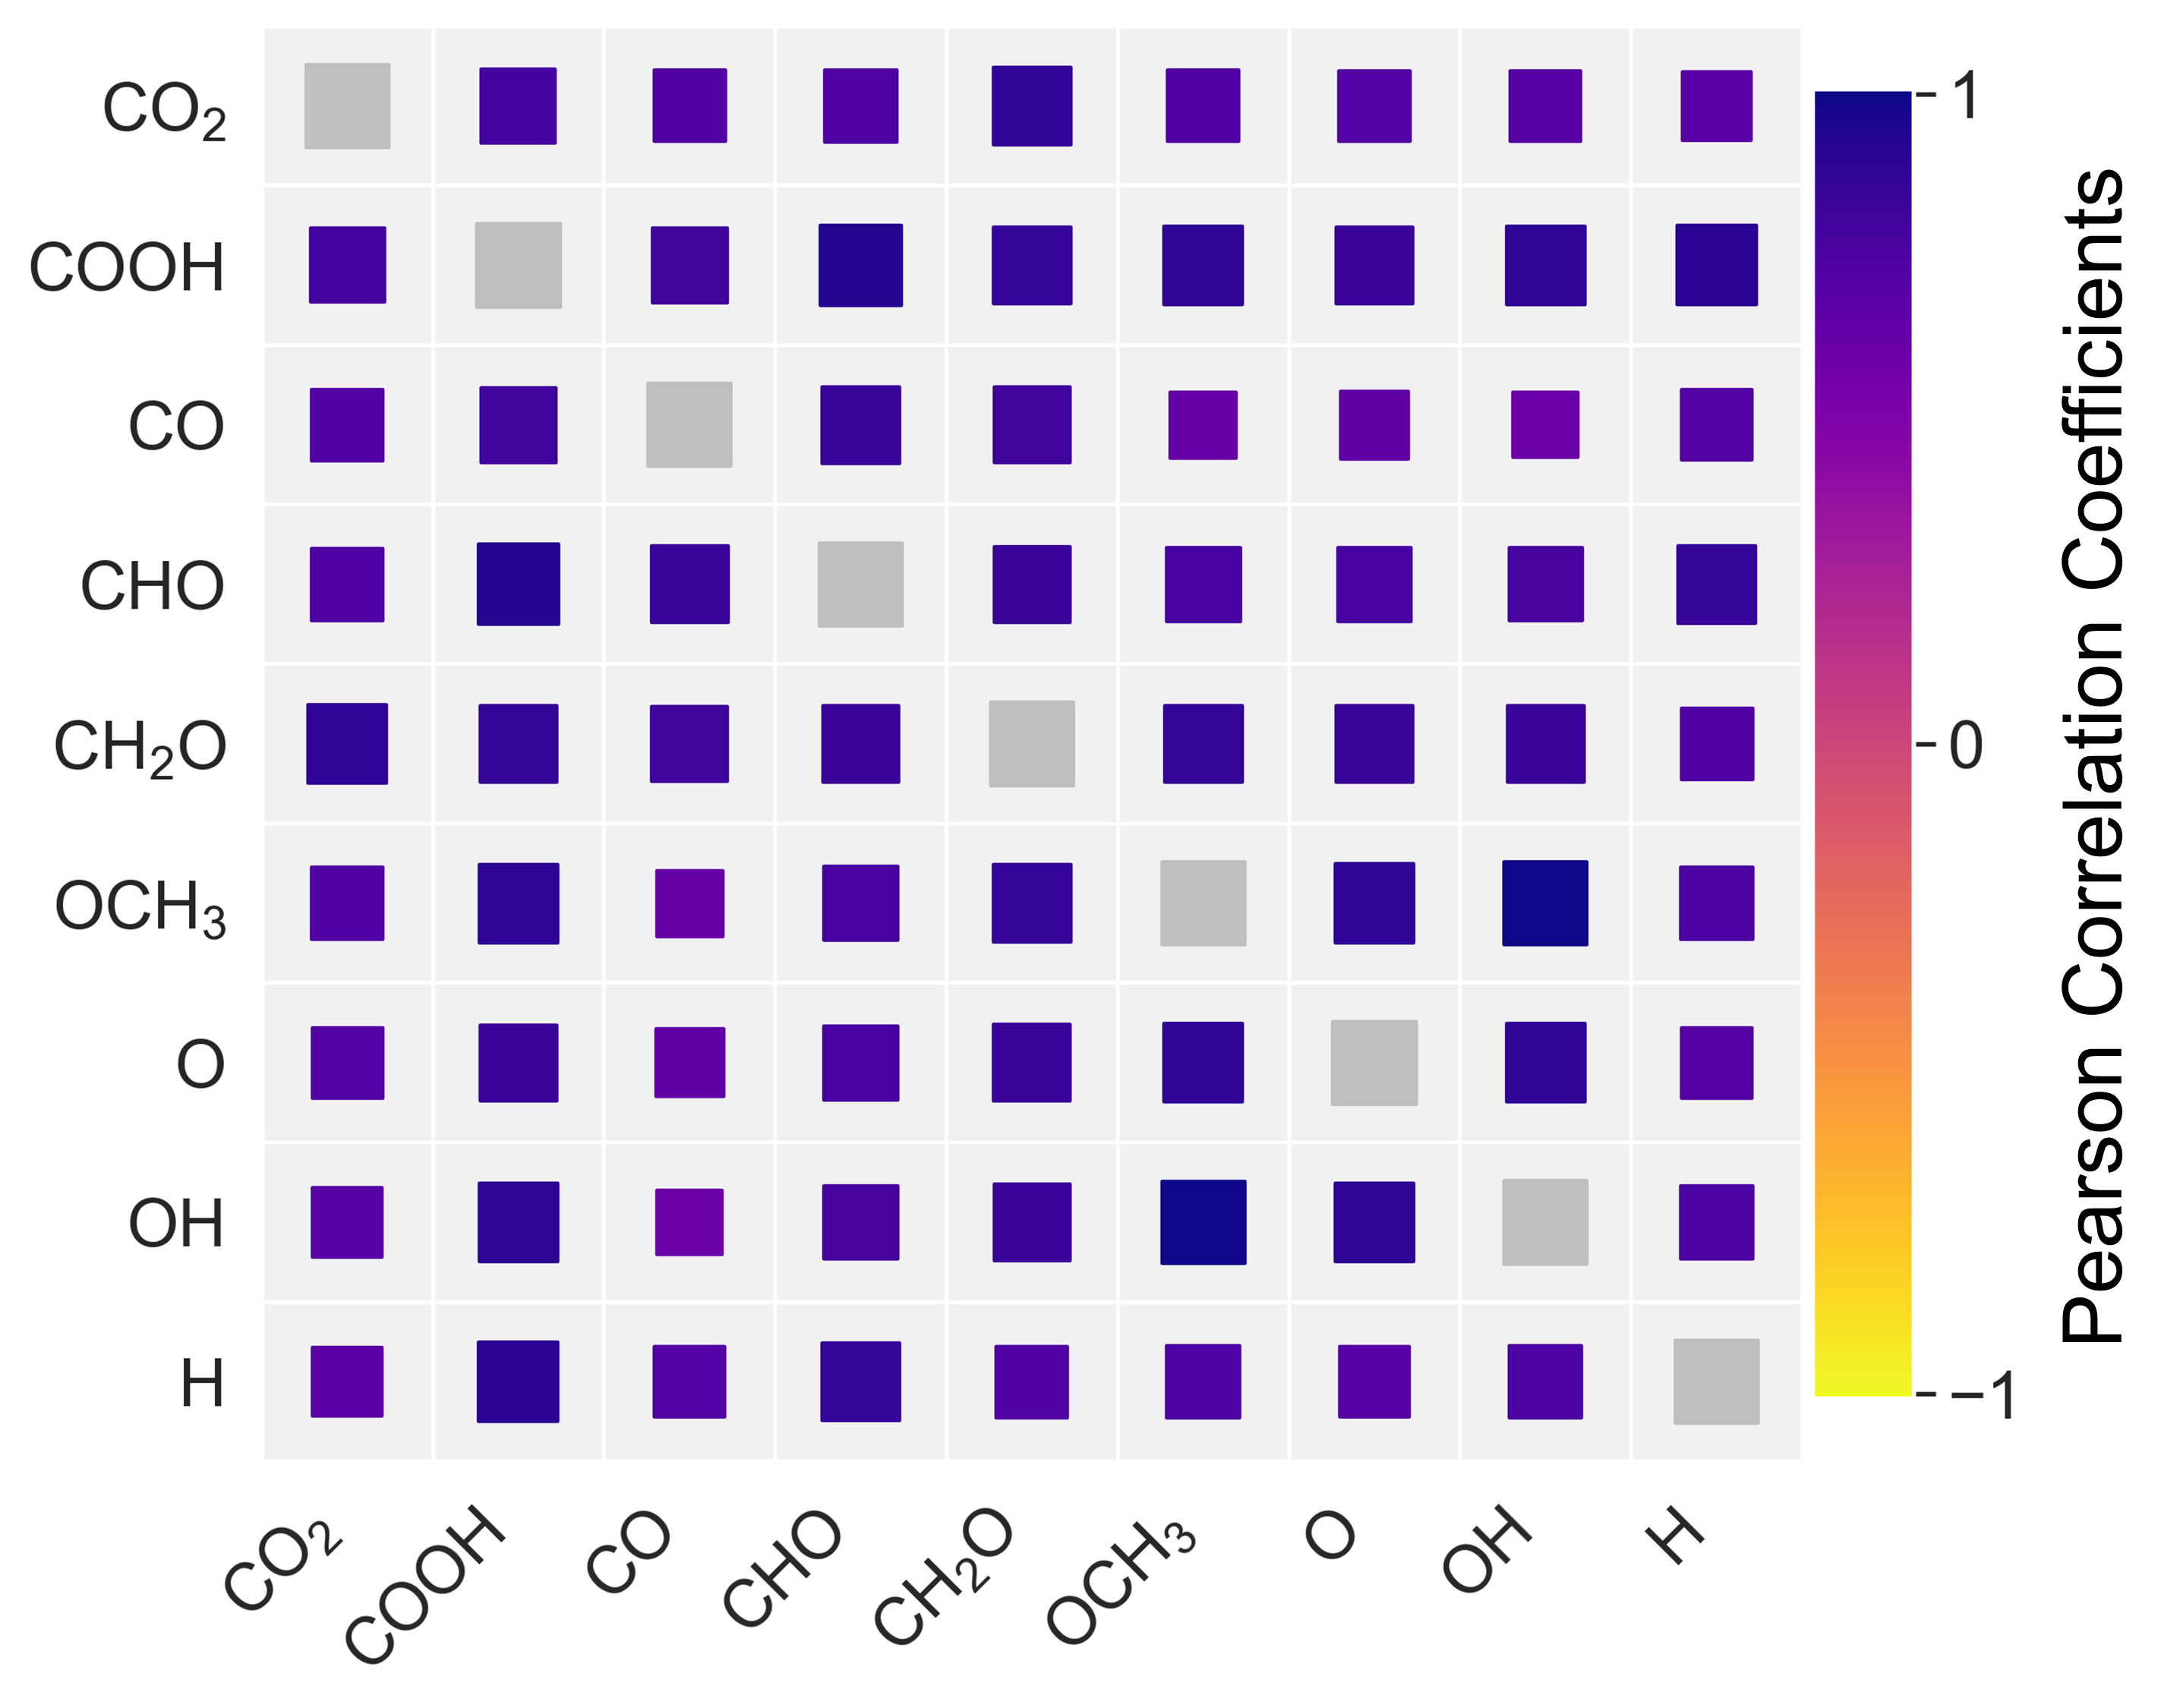
\includegraphics[width=0.7\textwidth]{supp_fig9_corr_eads.png}
  \caption{\textbf{Pearson correlation map for adsorption energies of various adsorbates for all six substrates.}}
  \label{supp_fig9:corr_eads}
\end{figure}

\subsection{The scaling relation scheme and the hybrid scaling relation}
\label{supp_sec2.5_scaling}

In line with the scaling relation framework proposed by Abild-Pedersen et al. \cite{abild2007scaling},
and later applied to the CO\textsubscript{2} reduction to methane process by Peterson \& Nørskov \cite{peterson2012activity},
adsorbates in the CO\textsubscript{2}RR process can be categorized into C-centered or O-centered species.
In each group, a representative species is designated as the ``descriptor'', allowing approximating the adsorption energies of other species within the same group using scaling relations.
The following equations capture this relationship:

\begin{align}
  G_{\text{ads}}X &= a_X \cdot G_{\text{ads}}{\text{CO}} + c_X
  && \text{(where  $X$ = COOH, CHO, CH\textsubscript{2}O)}  \label{supp_eq1:scaling_relation_x_co}  \\
  G_{\text{ads}}Y &= a_Y \cdot G_{\text{ads}}{\text{OH}} + c_Y
  && \text{(where  $Y$ = O, OCH\textsubscript{3})}          \label{supp_eq2:scaling_relation_y_oh}
\end{align}

Here, CO and OH serve as descriptors for C-centered ($X$) and O-centered ($Y$) groups, respectively, and $a_{\mathrm{X}}, c_{\mathrm{X}}, a_{\mathrm{Y}}, c_{\mathrm{Y}}$ are species-specific scaling parameters.
The scaling relations simplify the adsorption energy landscape to a two-dimensional space, thereby enabling visualization.

However, it's crucial to note that in the CO\textsubscript{2}RR process, most species are not solely C- or O-centered.
Thus, it becomes advantageous to incorporate both types of species in the scaling relation.
Building upon the hybrid scaling relation introduced in the main text, the free energy change ($\Delta\mathit{G}$) for any given reaction step can be readily calculated using \cref{main_eq14:general_scaling_relation} from the main text.
Consider the generic reaction step:
\begin{align}
  \ce{\text{*}A + H+ + e- -> \text{*}B}  \label{supp_eq3:generic_reaction}
\end{align}

The free energy change $\Delta\mathit{G}$ is defined as:
\begin{align}
  \Delta G = G(\text{*}\mathrm{B}) - G(\text{*}\mathrm{A}) - G(\mathrm{H}^+) - G(e^-)  \label{supp_eq4:free_energy_change}
\end{align}

Focusing on any reaction step delineated by \cref{main_eq1:co2rr1} to \cref{main_eq8:co2rr8} in the main text,
\cref{main_eq15:limiting_potential} shows that limiting potential $U_{\mathrm{L}}$ at a specific external potential $U$ is fully determined by the adsorption energies of two descriptors.
For instance, for the reaction described by \cref{main_eq2:co2rr2}:
\begin{align}
  \Delta G &= G(\text{*COOH}) - G(\text{*}) - G(\text{CO}_2) - G(\text{H}^+) - G(\text{e}^-)  \\
  &= G(\text{COOH}) + G(\text{*}) + G_{\text{ads}}\text{COOH} -
  G(\text{*}) - G(\text{CO}_2) -G(\text{H}^+) - G(\text{e}^-) \\
  &= G_{\text{ads}}\text{COOH} + G(\text{COOH}) - G(\text{CO}_2) -G(\text{H}^+) - G(\text{e}^-)  \label{supp_eq5:exp_reaction}
\end{align}

From adsorption energy linear relations, we have:
\begin{align}
  G_{ads}{\mathrm{COOH}} = a_{\text{COOH}} \cdot G_{ads}{\mathrm{CO}} +
  b_{\text{COOH}} \cdot G_{ads}{\mathrm{OH}} + c_{\text{COOH}}  \label{supp_eq6:eads}
\end{align}

which then reduces Supplementary \cref{supp_eq5:exp_reaction} to:
\begin{align}
  \begin{split}
    \Delta G = &(a_{\text{COOH}} \cdot G_{\text{ads}}{\mathrm{CO}} +
    b_{\text{COOH}} \cdot G_{\text{ads}}{\mathrm{OH}}) + \\
    &[c_{\text{COOH}} + G(\mathrm{COOH}) -
    G(\mathrm{CO}_2) - G(\mathrm{H}^+) - G(\mathrm{e}^-)]  \label{supp_eq7:reduced_eads}
  \end{split}
\end{align}
In this case, the first term depends solely on the descriptors, while the second term remains constant at a given potential $U$.

% Supplementary Table 13: Eads scaling relation params from hybrid descriptor method
\begin{table}[htbp]
\label{supp_table13:scaling_params}
  \caption{Adsorption free energy scaling relation parameters
    determined by the hybrid descriptor method.}
  \small
  \begin{tabularx}{\textwidth}{@{}l *{3}{X} @{}}
    \toprule
    Adsorbate             & $a_Z$   & $b_Z$   & $c_Z$    \\
    \midrule
    COOH                  & 0.4032  & 0.5132  &  0.0899  \\
    CHO                   & 0.5977  & 0.3664  & -2.6763  \\
    CH\textsubscript{2}O  & 0.5011  & 0.5011  & -0.9806  \\
    OCH\textsubscript{3}  & 0.0532  & 1.0114  &  0.8489  \\
    O                     & 0.3758  & 1.2580  &  0.0910  \\
    H                     & 0.3164  & 0.3568  & -0.6764  \\
    \bottomrule
  \end{tabularx}

  \smallskip

  \footnotesize\textit{Note:} $a_{Z}$, $b_{Z}$ and $c_{Z}$ correspond
    to coefficients for $G_{\text{ads}}\text{CO}$, $G_{\text{ads}}\text{OH}$
    and constant terms, where $Z$ stands for the adsorbed species of interest.
\end{table}

% SI Figure 10: Improvement in R2 from hybrid-descriptor method
\begin{figure}[htbp]
  \centering
  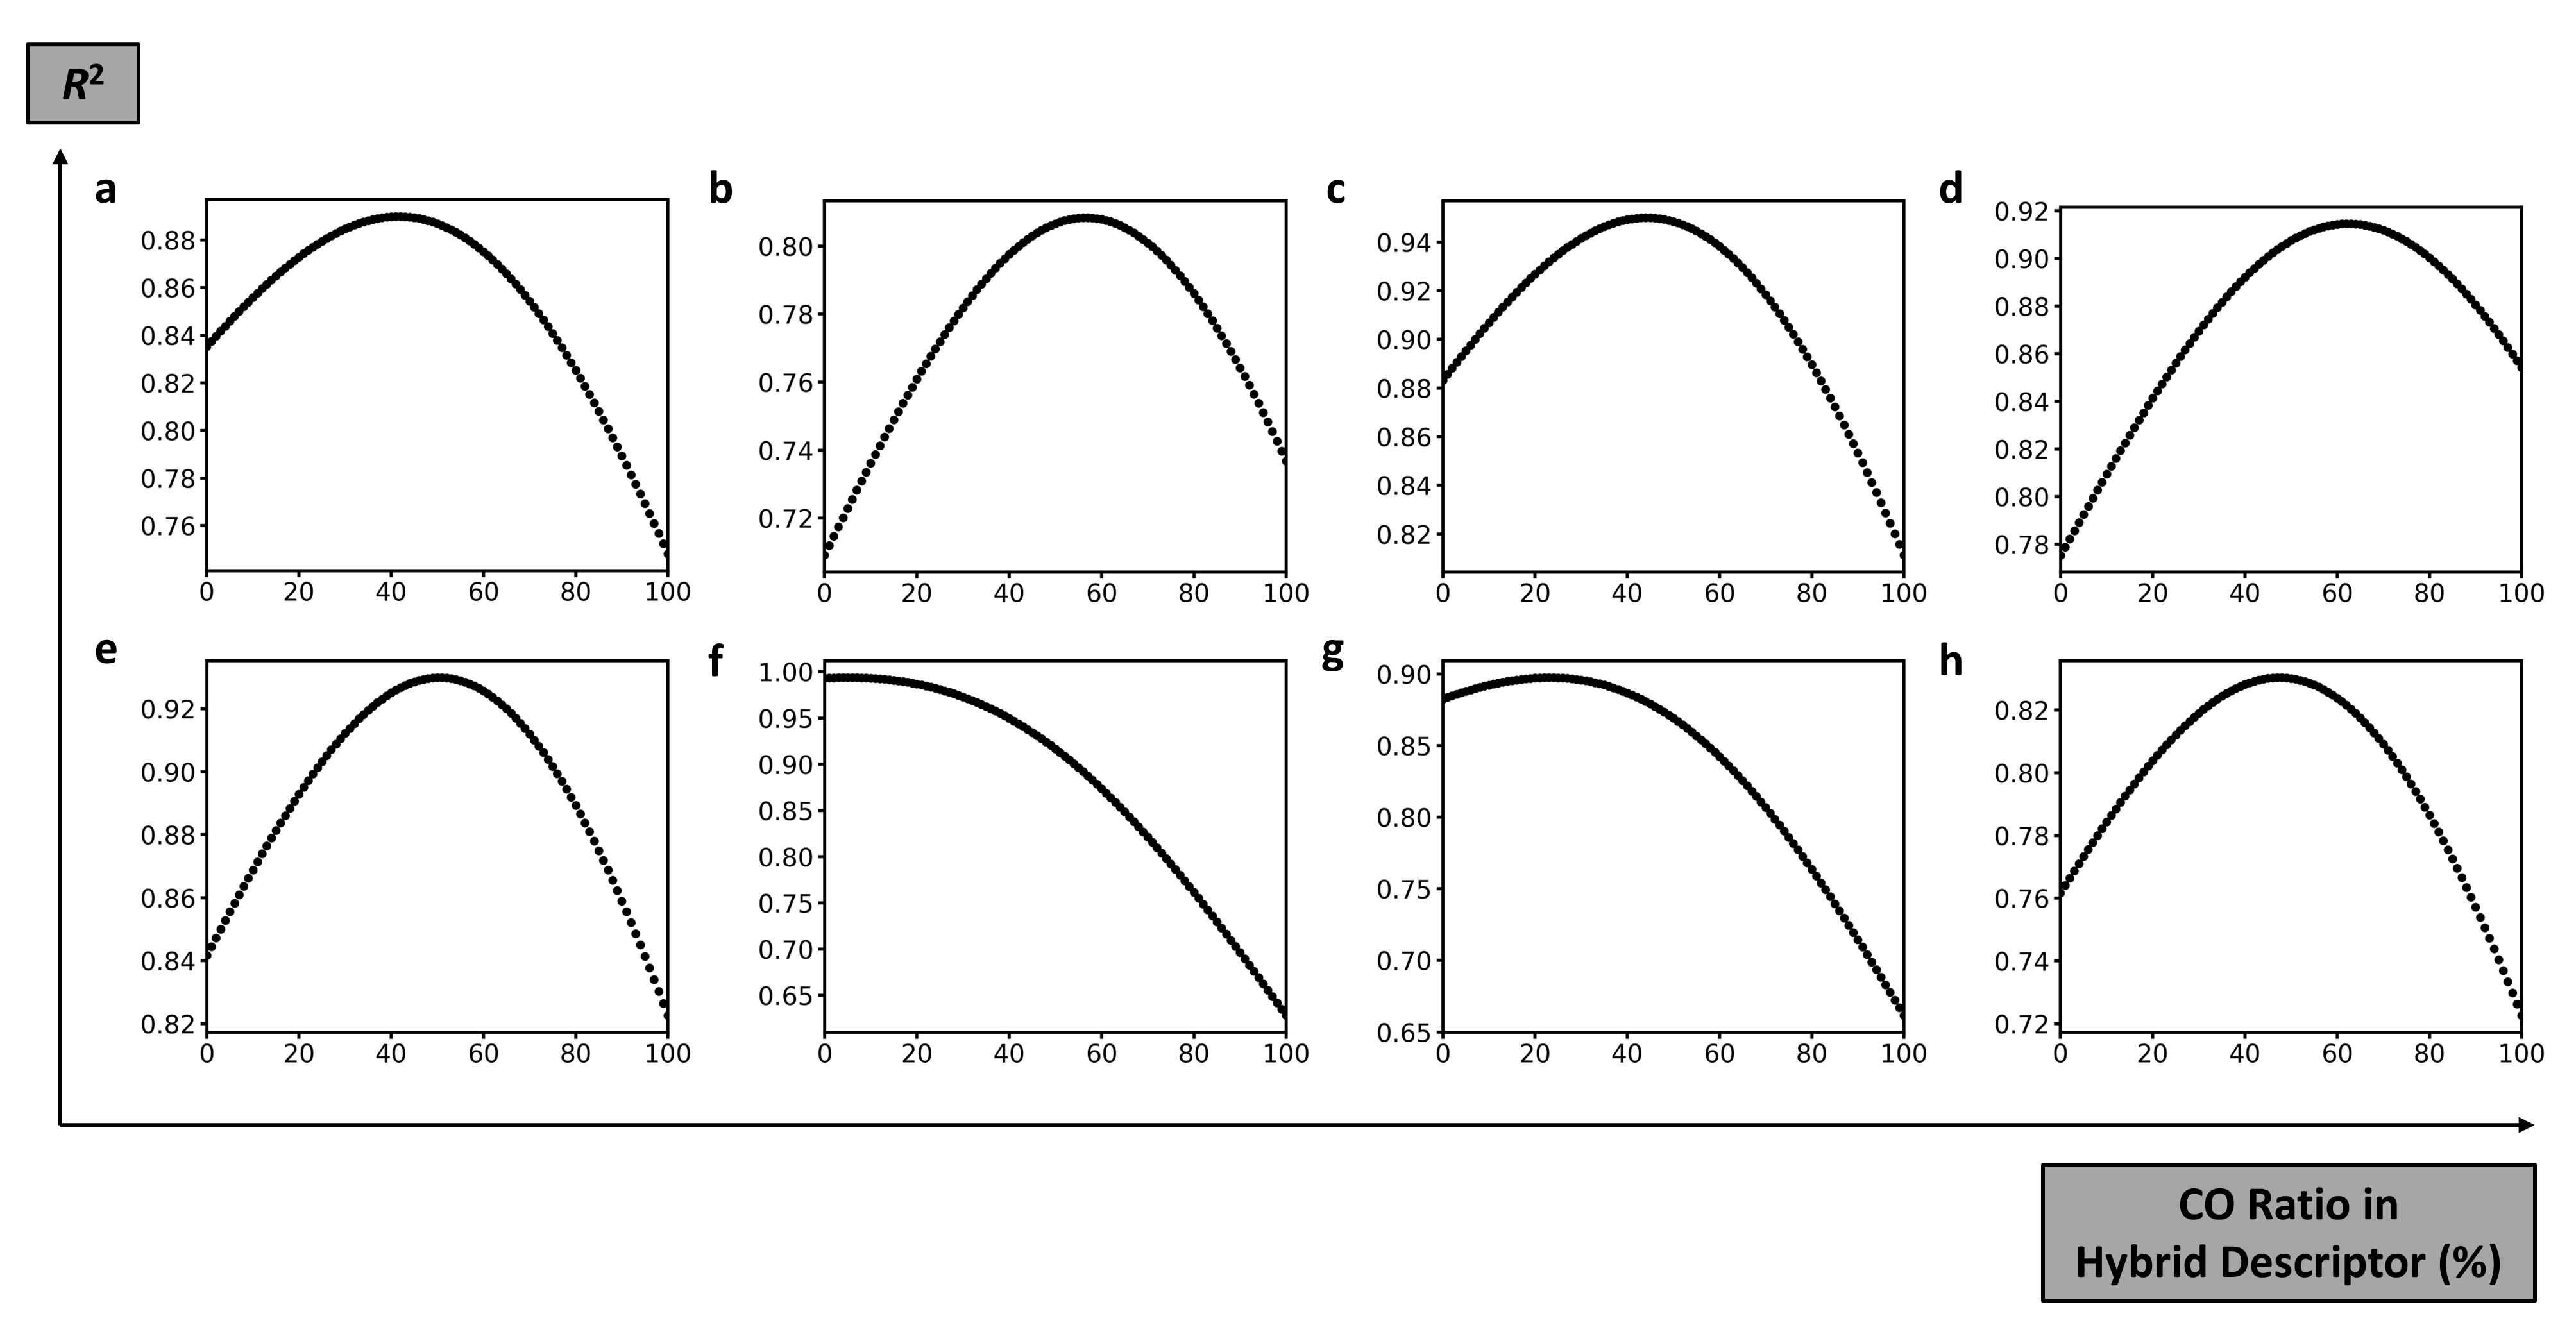
\includegraphics[width=\textwidth]{supp_fig10_r2_hyb_des.png}
  \caption{\textbf{$R^2$ improvement from hybrid-descriptor method.}
  Improvement in the coefficient of determination ($R^2$) with x-axis
  as CO ratio in CO/OH hybrid descriptors.
  (\textbf{a}) averaged $R^2$ and those of (\textbf{b}) CO\textsubscript{2},
  (\textbf{c}) COOH,
  (\textbf{d}) CHO, (\textbf{e}) CH\textsubscript{2}O, (\textbf{f})
  OCH\textsubscript{3}, (\textbf{g}) O and (\textbf{h}) H are shown.}
  \label{supp_fig10:r2_hyb_des}
\end{figure}

% Supplementary Table 14: Performance comparison of hybrid/single descriptors
\begin{table}[htbp]
\label{supp_table14:hybrid_des_perf}
  \caption{Performance comparison of hybrid descriptor and single
    descriptor for linear scaling relations.}
  \small
  \begin{tabularx}{\textwidth}{@{}l *{3}{X} @{}}
    \toprule
    \multirow{2}{*}{Adsorbate} & Hybrid Descriptor $R^2$ & Single Descriptor $R^2$ & \multirow{2}{*}{$R^2$} \\
                               & (Optimal CO Ratio)      & Reference Species       &                        \\
    \midrule
    CO\textsubscript{2}   & 0.8083 (57\%)  & 0.7368 (CO)  & 0.0715  \\
    COOH                  & 0.9500 (44\%)  & 0.8113 (CO)  & 0.1387  \\
    CHO                   & 0.9146 (62\%)  & 0.8541 (CO)  & 0.0605  \\
    CH\textsubscript{2}O  & 0.9299 (50\%)  & 0.8226 (CO)  & 0.1073  \\
    OCH\textsubscript{3}  & 0.9936 (5\%)   & 0.9929 (OH)  & 0.0007  \\
    O                     & 0.8974 (23\%)  & 0.8825 (OH)  & 0.0149  \\
    H                     & 0.8303 (47\%)  & 0.7617 (OH)  & 0.0686  \\
    \bottomrule
  \end{tabularx}
\end{table}

\subsection{Volcano plots}
\label{supp_sec2.6_volcano}

In addition to the selectivity volcano plot featured in the main text, we provide a comprehensive plot capturing all rate-determining steps for CO\textsubscript{2}RR in \cref{supp_fig11:rds_volcano}. A separate plot focusing on selectivity over HER is also presented in \cref{supp_fig12:sel_volc}.

% SI Figure 11: CO2RR rate determining step volcano plot
\begin{figure}[htbp]
  \centering
  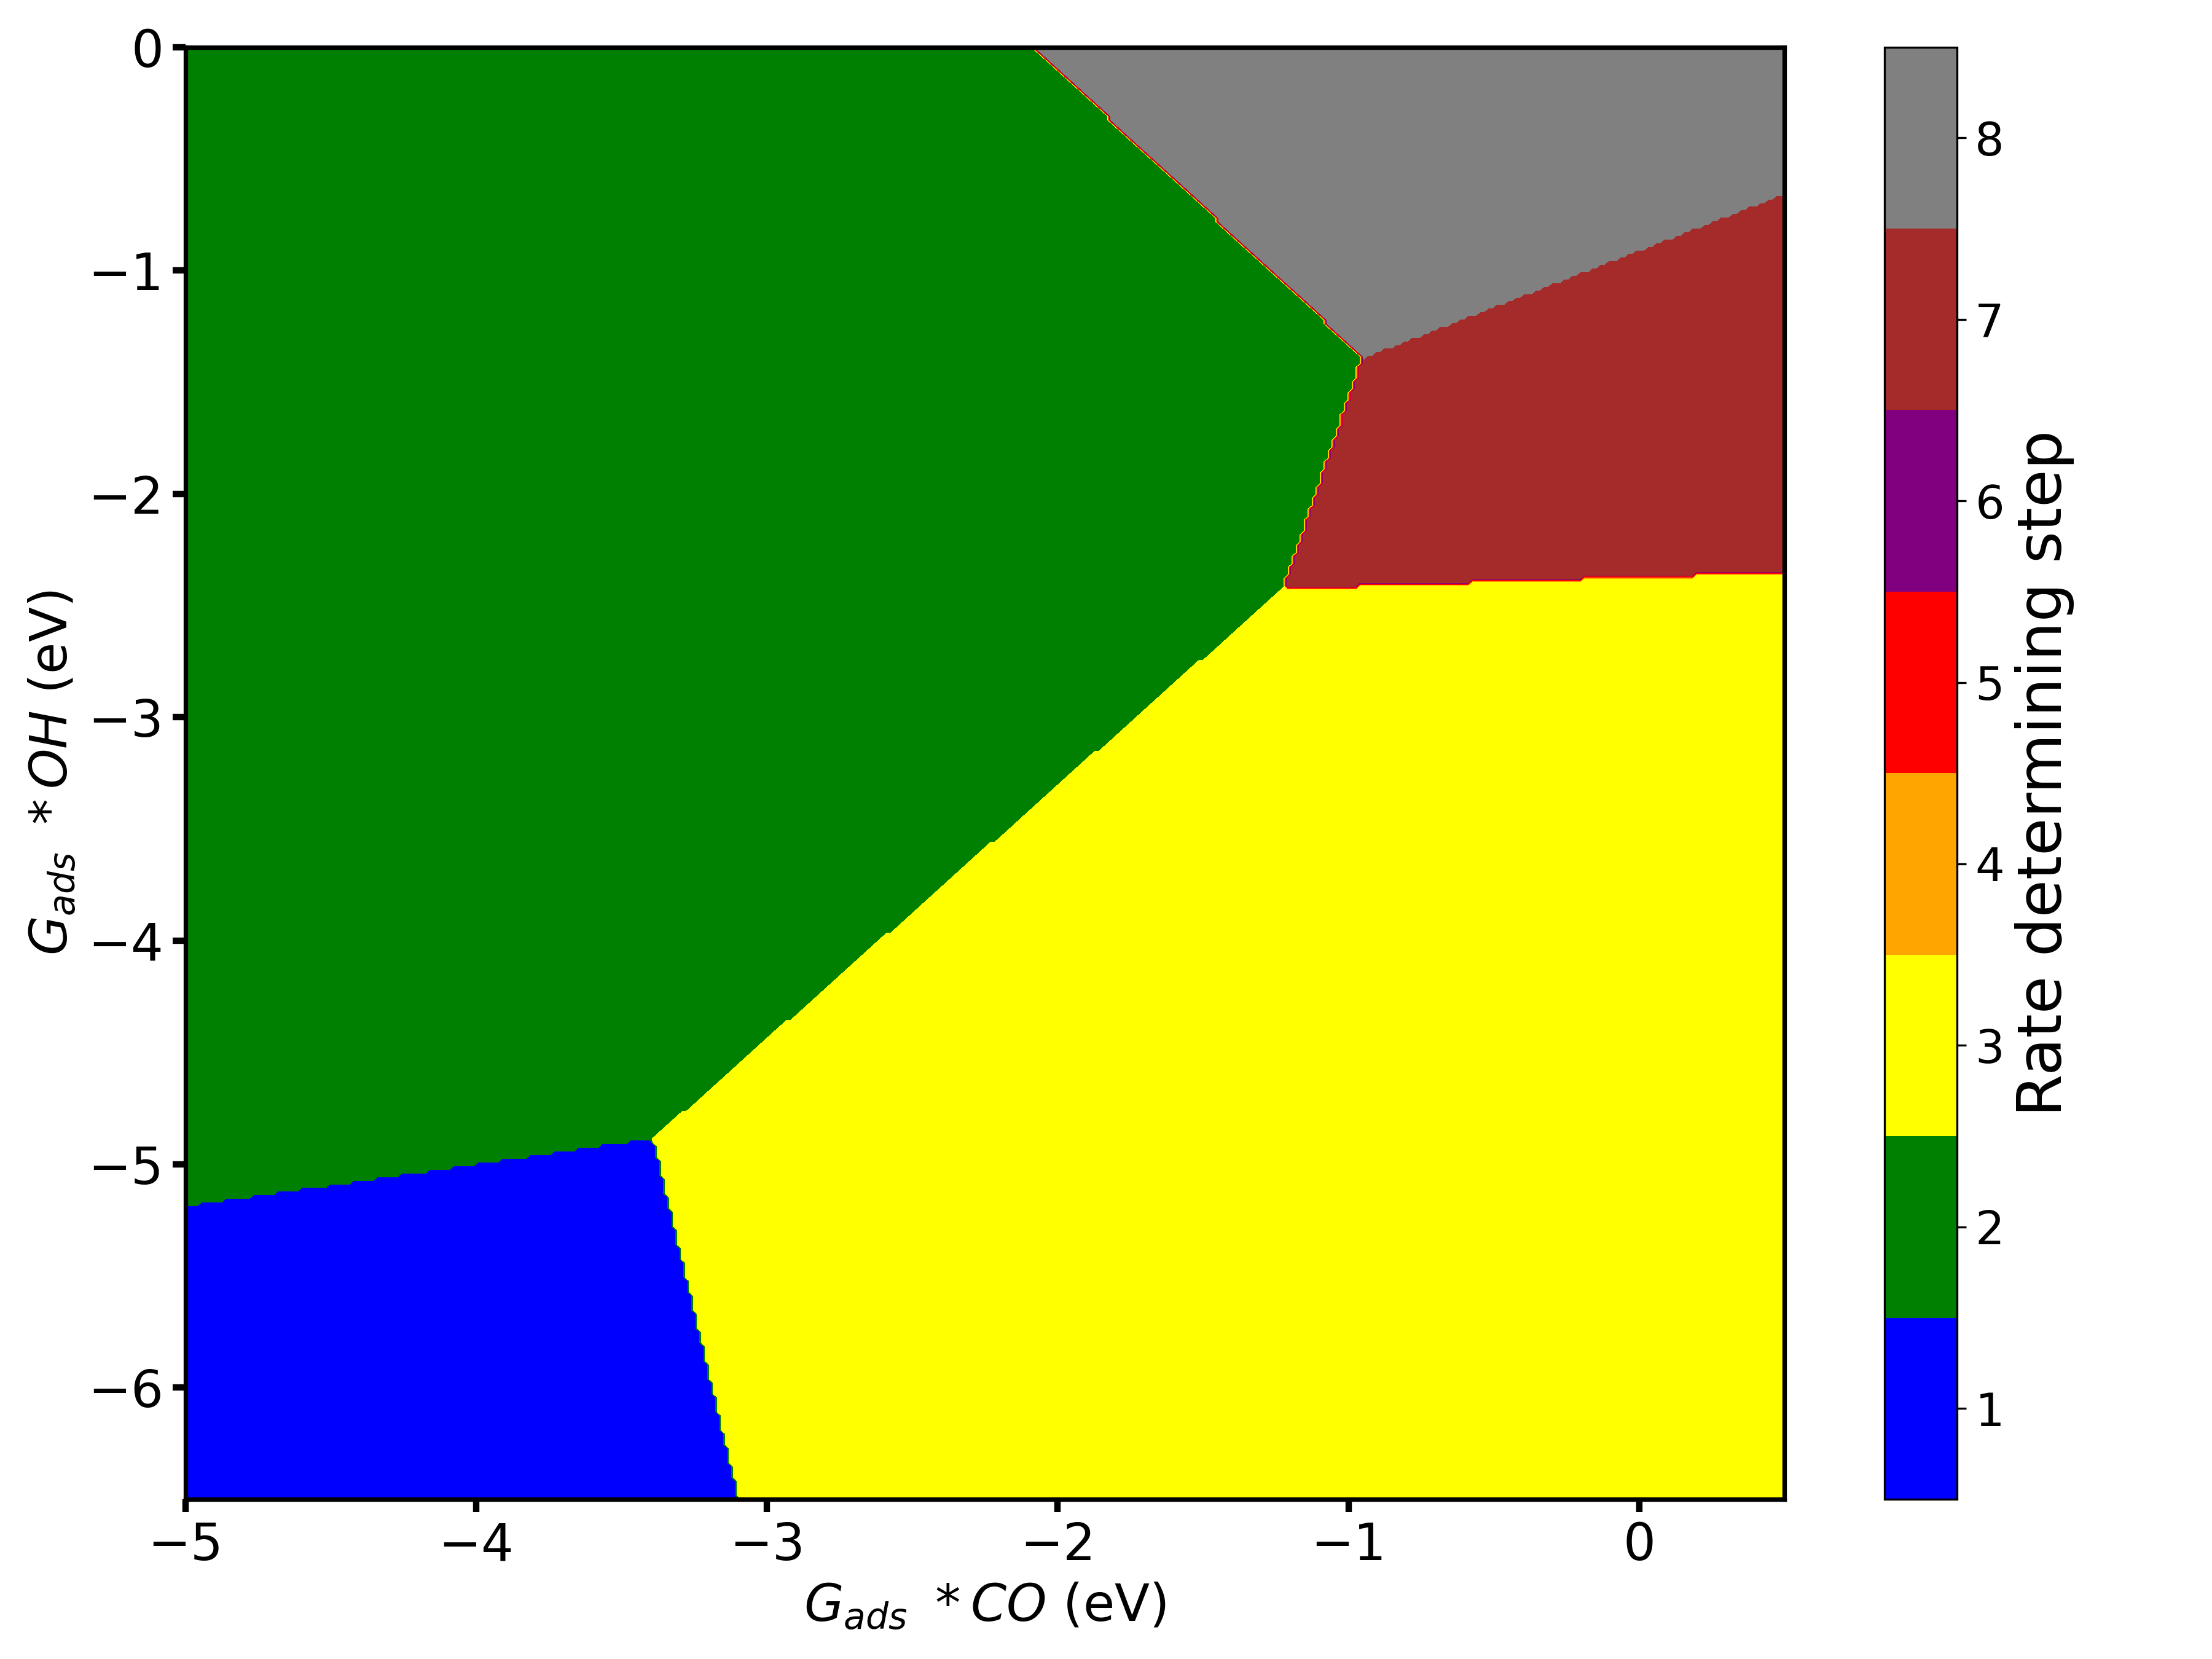
\includegraphics[width=\textwidth]{supp_fig11_rds_volcano.png}
  \caption{\textbf{CO\textsubscript{2}RR rate determining step volcano plot.}
  This graph illustrates the rate-determining step associated with each region within the CO\textsubscript{2}RR process.}
  \label{supp_fig11:rds_volcano}
\end{figure}

% SI Figure 12: CO2RR selectivity volcano plot
\begin{figure}[htbp]
  \centering
  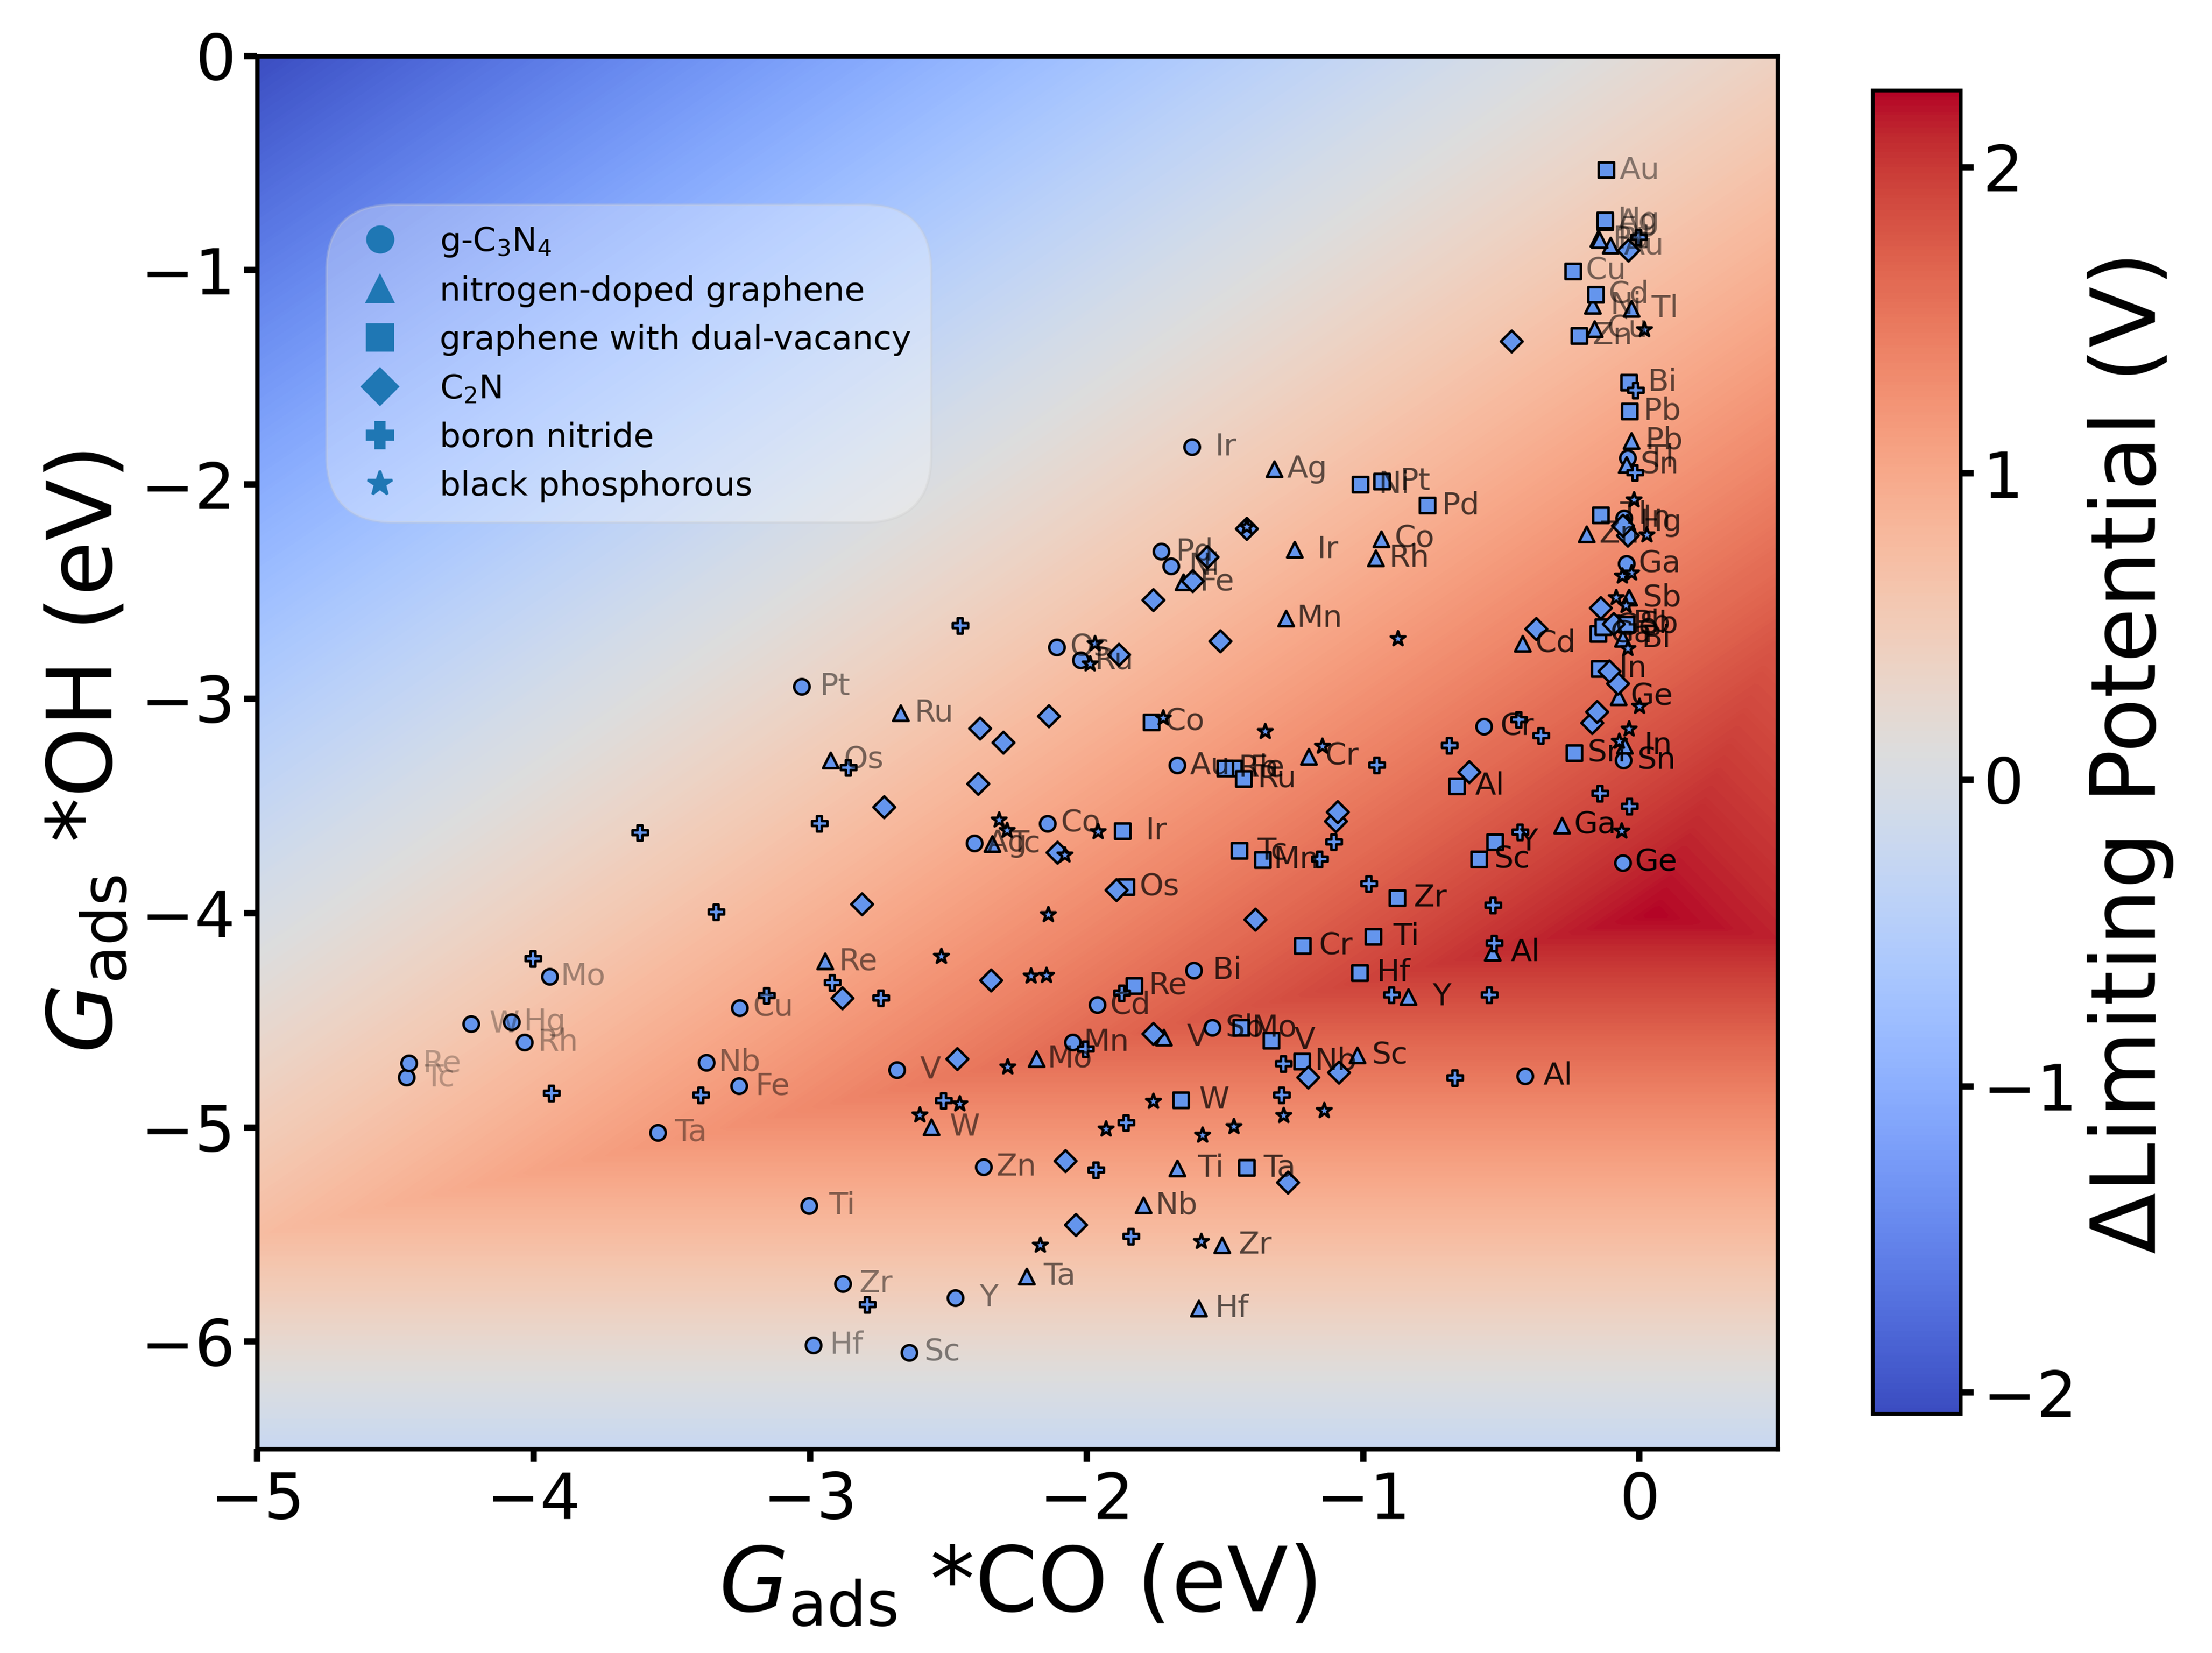
\includegraphics[width=\textwidth]{supp_fig12_sel_volc.png}
  \caption{\textbf{CO\textsubscript{2}RR selectivity volcano plot.}
  Selectivity volcano plot computed from linear scaling relations.
  In the plot, the circle, triangle, square, diamond, plus, and star symbols correspond to
  metals supported on g-C\textsubscript{3}N\textsubscript{4}, nitrogen-doped graphene, graphene with dual-vacancy,
  black phosphorous, BN, and C\textsubscript{2}N, respectively.}
  \label{supp_fig12:sel_volc}
\end{figure}

\subsection{Activity periodic tables}
\label{supp_sec2.7_ptable}

% SI Figure 13: Limiting potential periodic table for nitrogen-doped graphene
\begin{figure}[htbp]
  \centering
  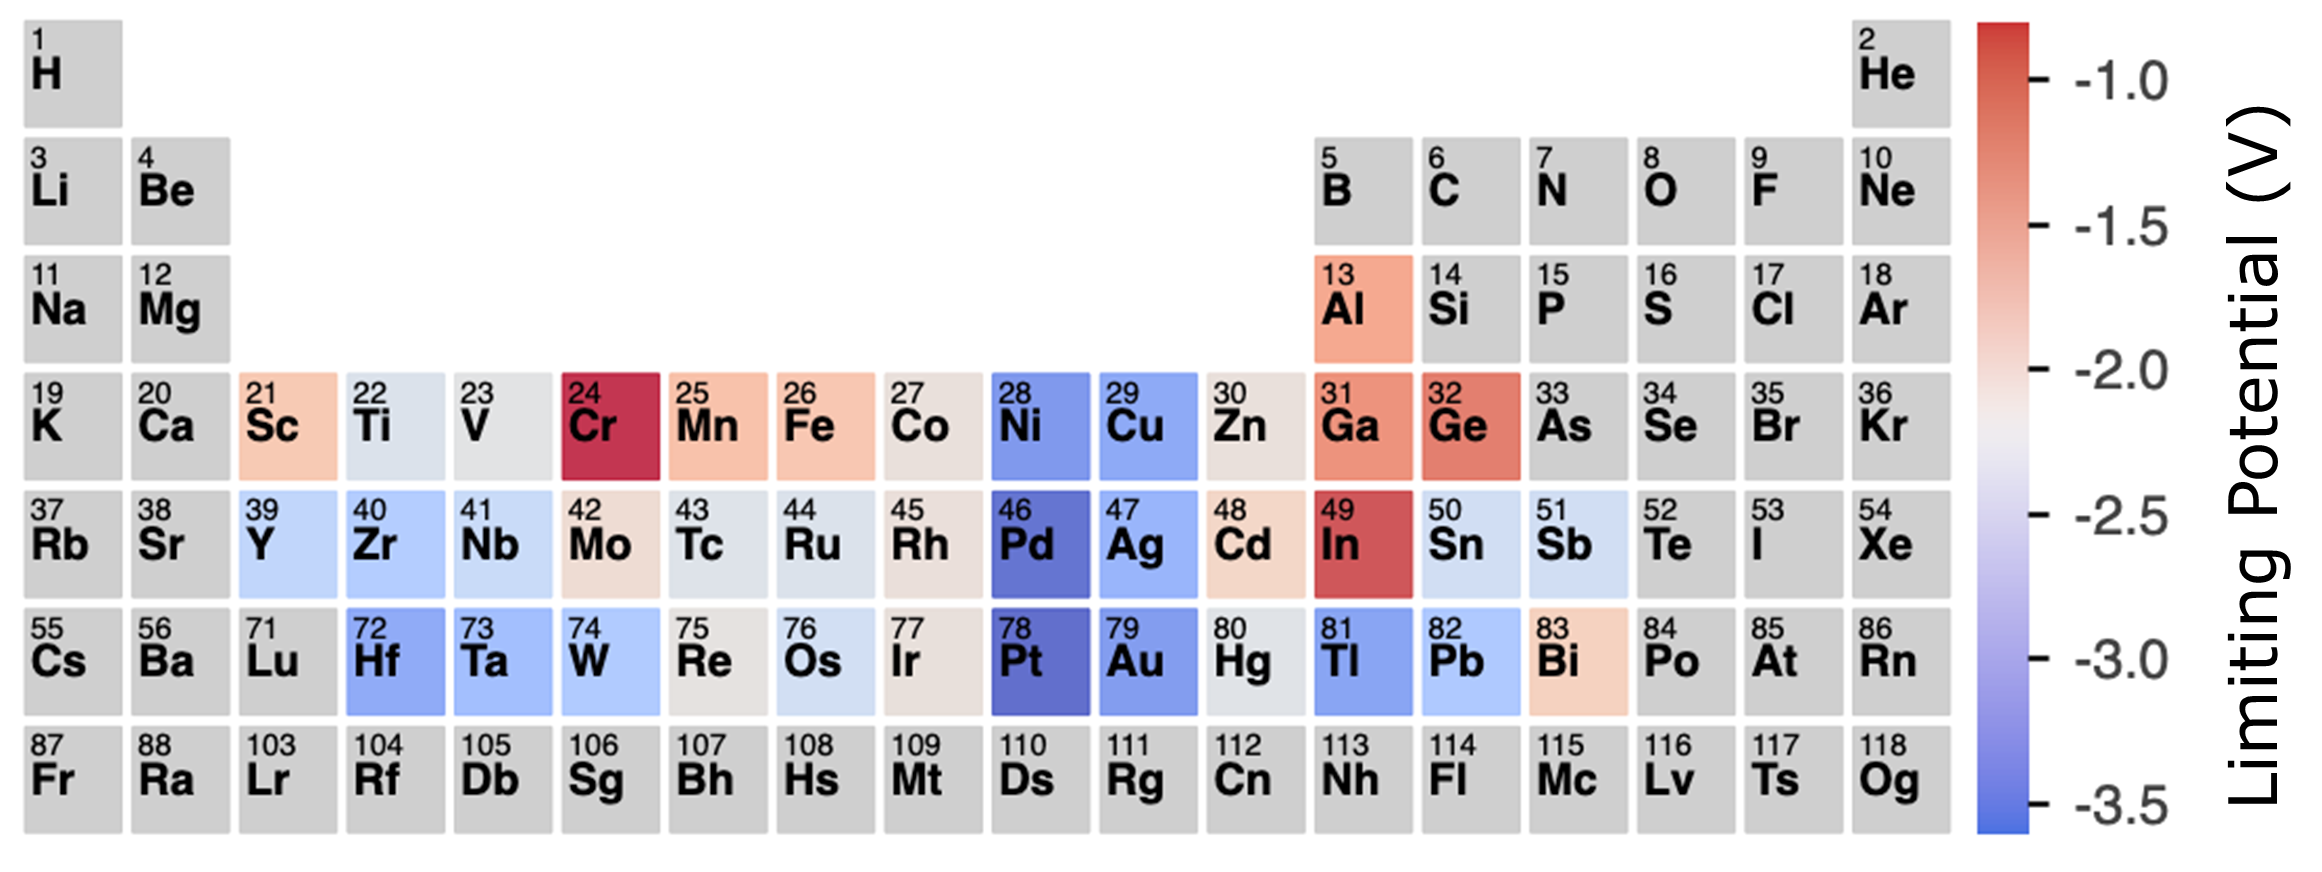
\includegraphics[width=\textwidth]{supp_fig13_n-gra_ptable.png}
  \caption{\textbf{Limiting potential periodic table for nitrogen-doped graphene.}}
  \label{supp_fig13:n-gra_ptable}
\end{figure}

% SI Figure 14: Limiting potential periodic table for graphene with dual-vacancy
\begin{figure}[htbp]
  \centering
  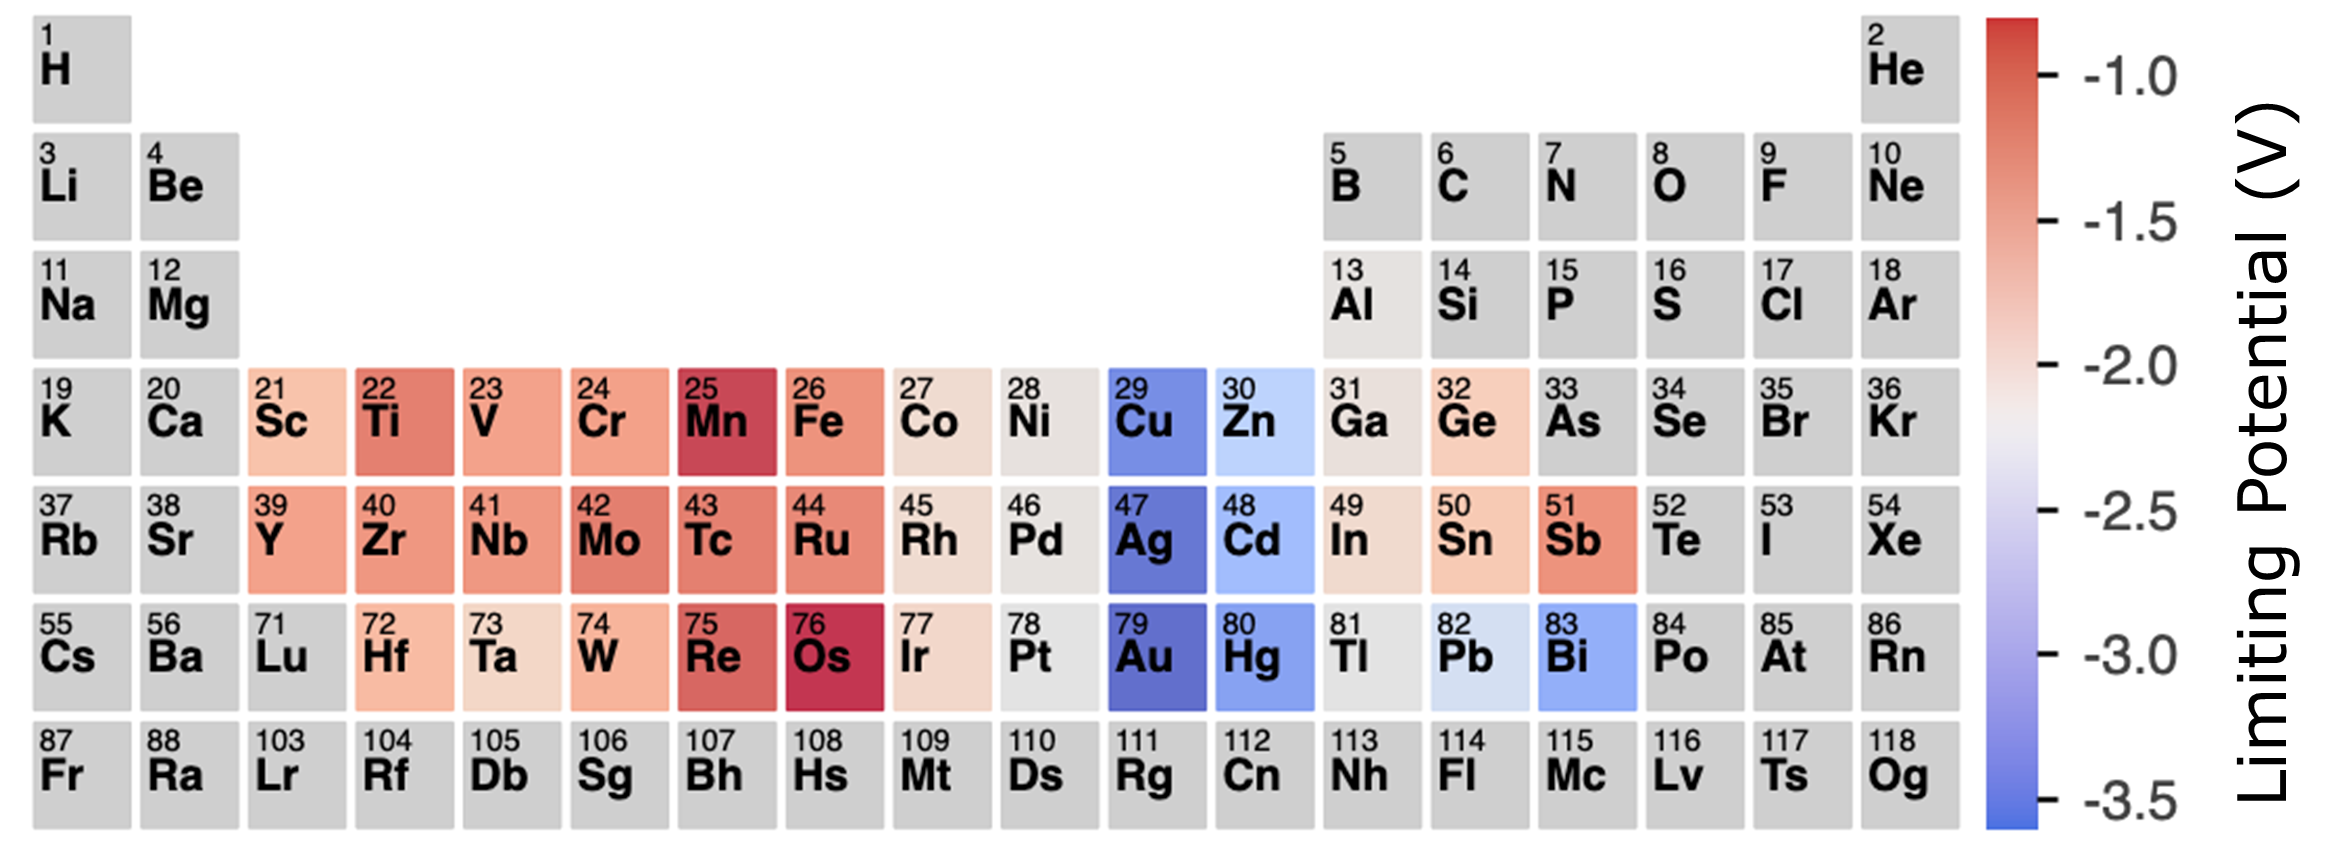
\includegraphics[width=\textwidth]{supp_fig14_gra-vac_ptable.png}
  \caption{\textbf{Limiting potential periodic table for graphene with dual-vacancy.}}
  \label{supp_fig14:gra-vac_ptable}
\end{figure}

% SI Figure 15: Limiting potential periodic table for black phosphorus
\begin{figure}[htbp]
  \centering
  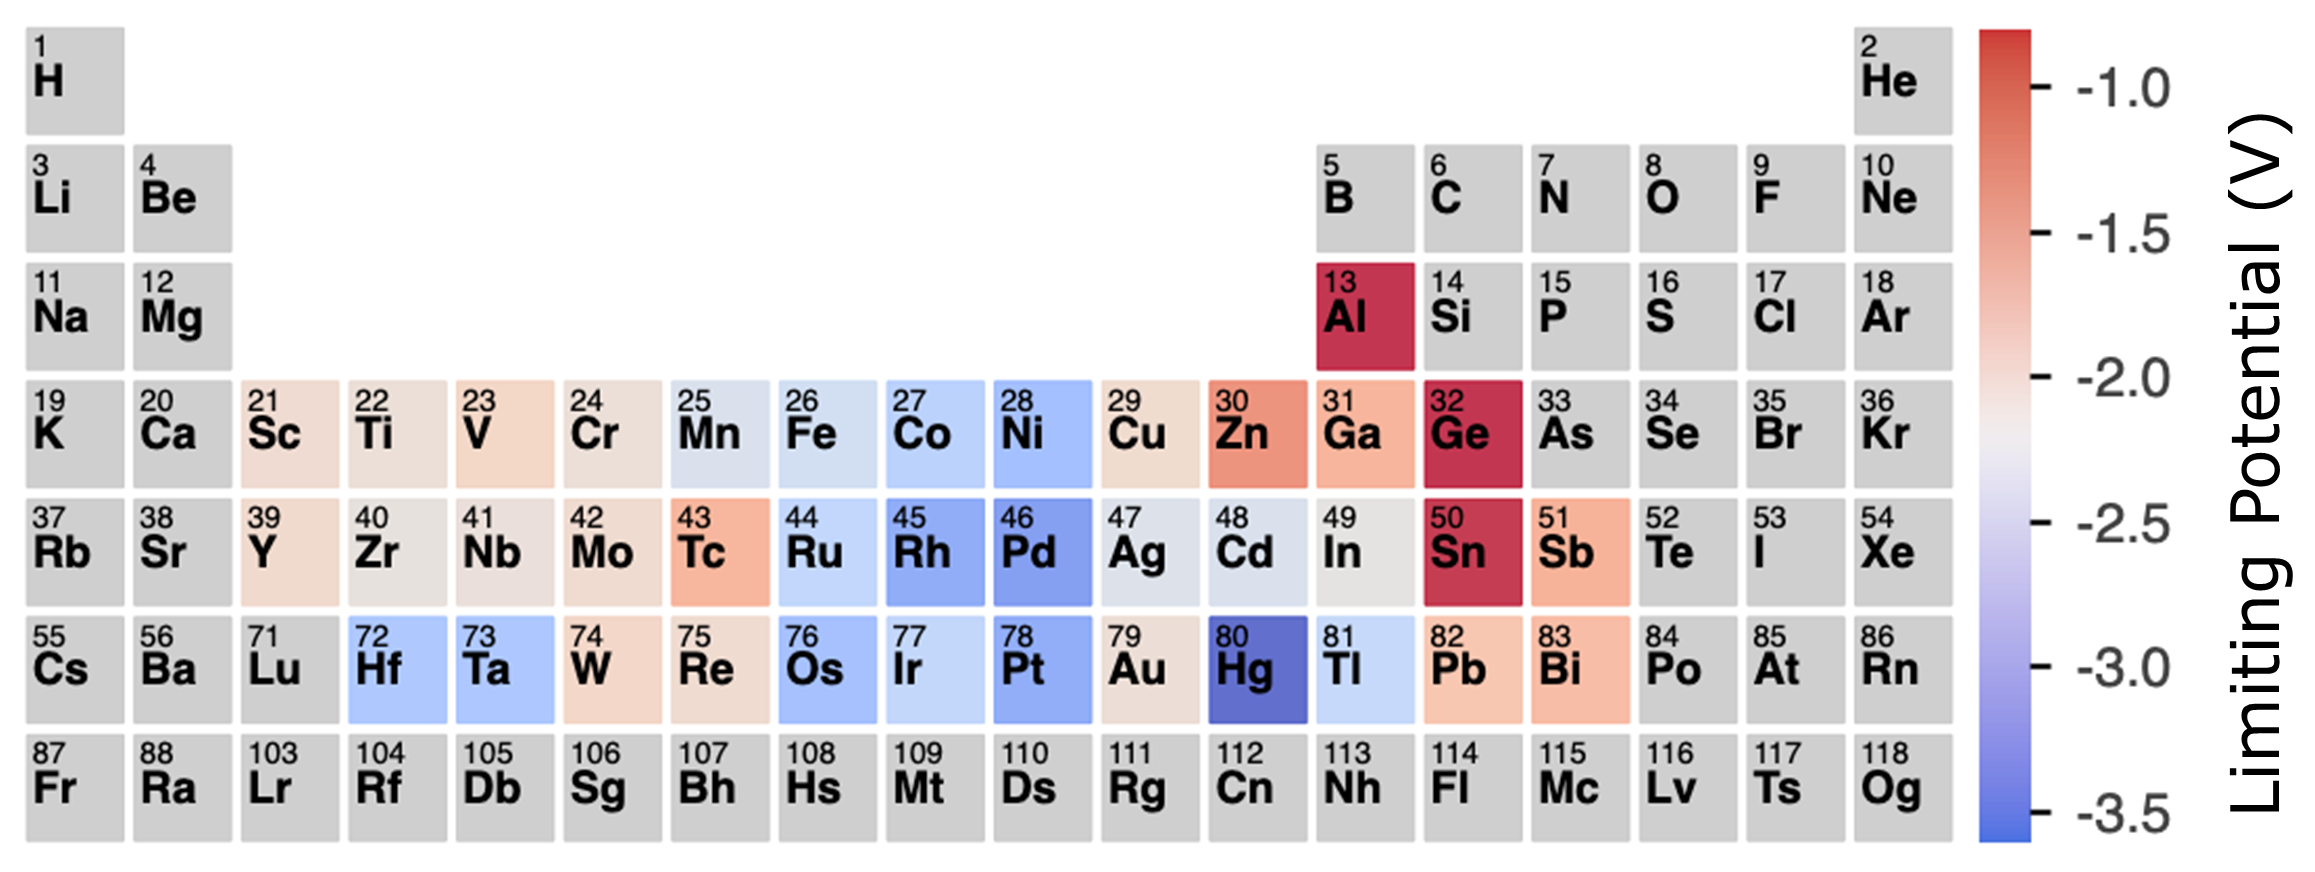
\includegraphics[width=\textwidth]{supp_fig15_BP_ptable.png}
  \caption{\textbf{Limiting potential periodic table for black phosphorus.}}
  \label{supp_fig15:BP_ptable}
\end{figure}

% SI Figure 16: Limiting potential periodic table for boron nitride
\begin{figure}[htbp]
  \centering
  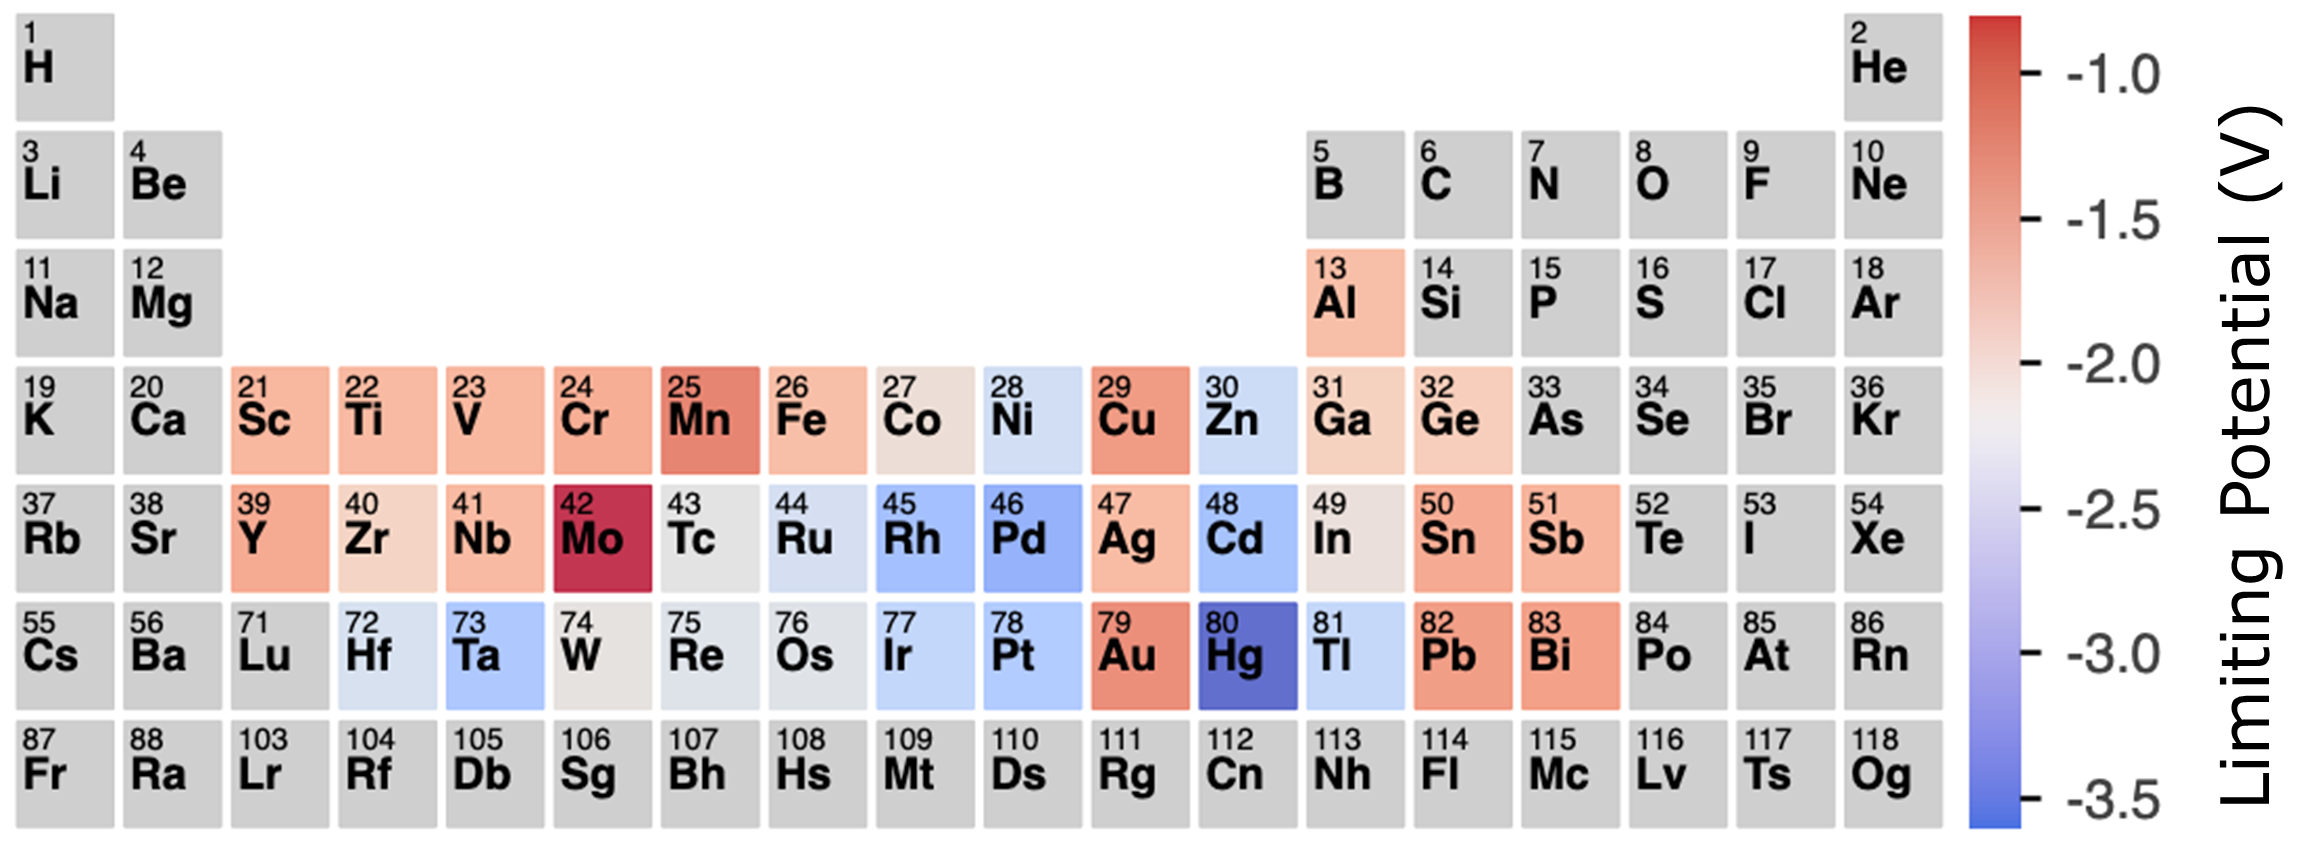
\includegraphics[width=\textwidth]{supp_fig16_BN_ptable.png}
  \caption{\textbf{Limiting potential periodic table for boron nitride.}}
  \label{supp_fig16:BN_ptable}
\end{figure}

% SI Figure 17: Limiting potential periodic table for monolayer C2N
\begin{figure}[htbp]
  \centering
  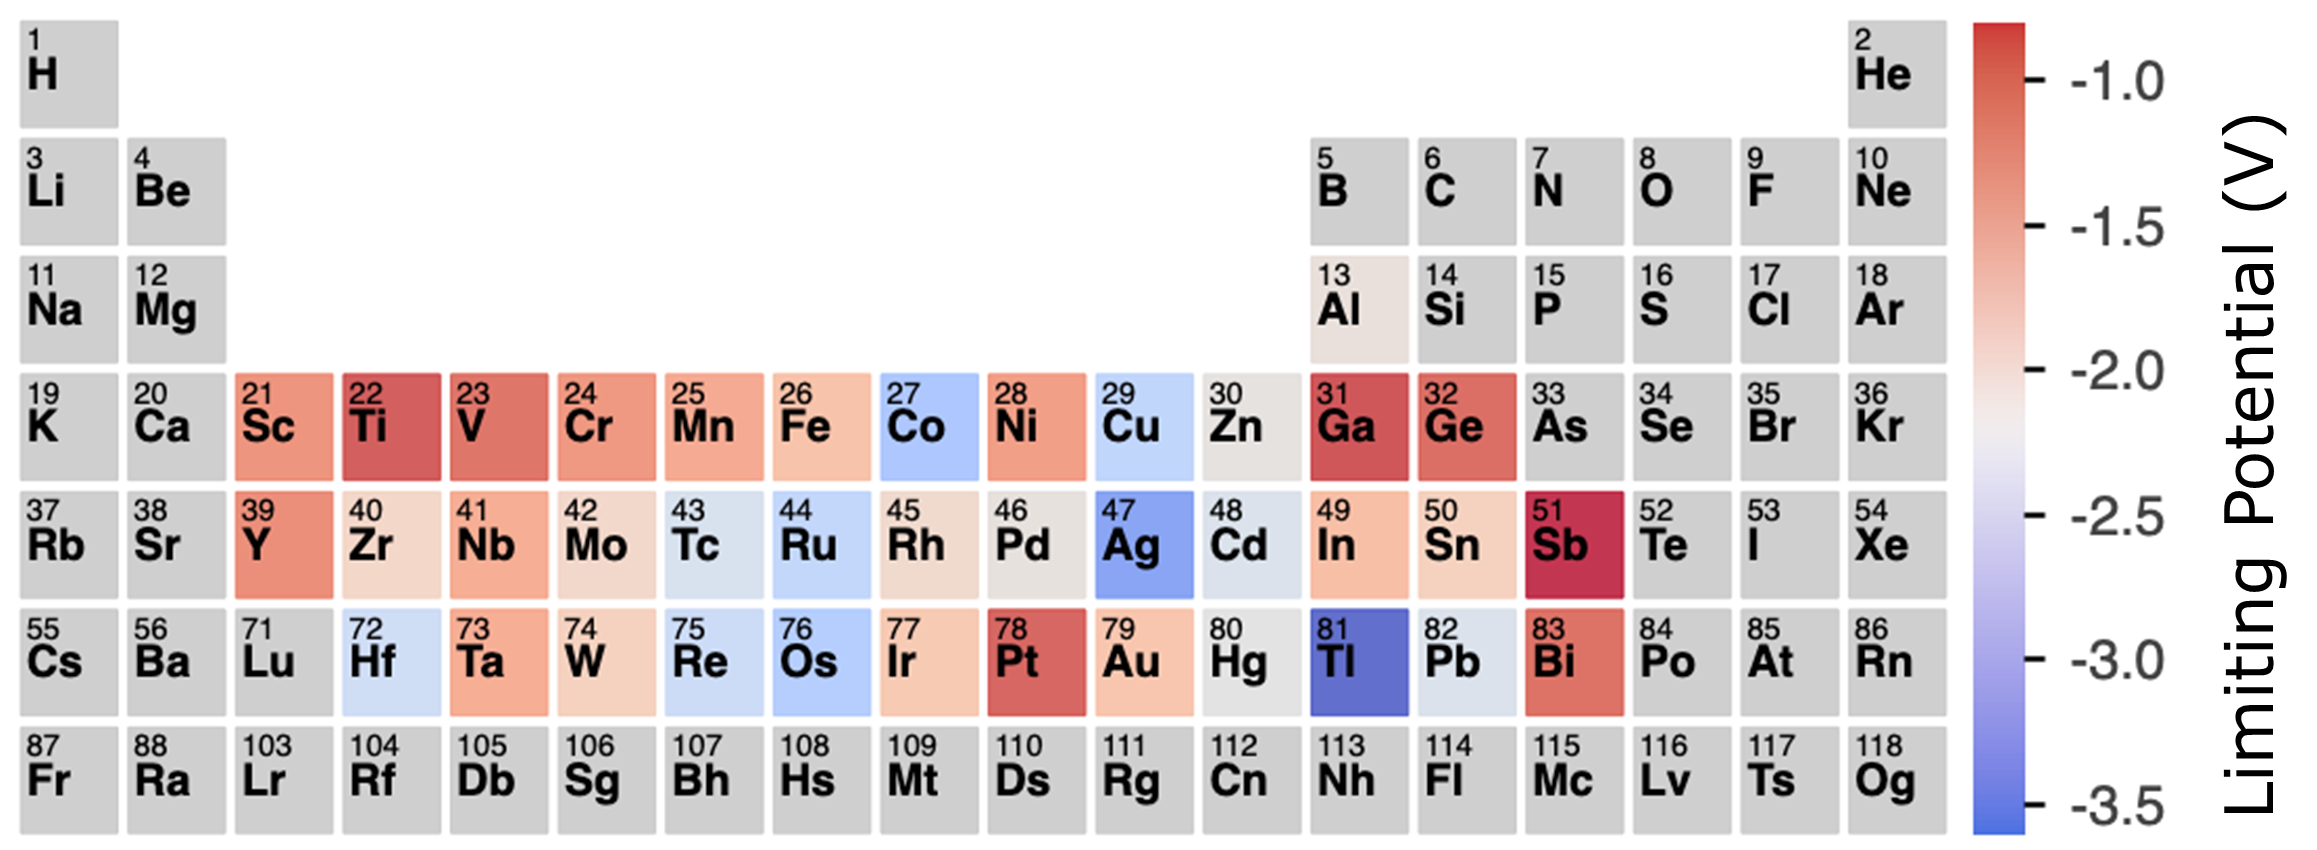
\includegraphics[width=\textwidth]{supp_fig17_C2N_ptable.png}
  \caption{\textbf{Limiting potential periodic table for monolayer C\textsubscript{2}N.}}
  \label{supp_fig17:C2N_ptable}
\end{figure}
